\documentclass[a4paper,12pt]{book}
\usepackage{parskip}
\usepackage[utf8]{inputenc}
\usepackage[sfdefault]{atkinson}
\usepackage[]{xcolor}
\definecolor{E}{RGB}{128, 32, 0}
\definecolor{O}{RGB}{0, 0, 255}
\definecolor{M}{RGB}{0, 128, 0}
\usepackage[super]{nth}
\usepackage{fancyhdr}
\renewcommand{\chaptername}{Section}
\usepackage[titletoc]{appendix}
\usepackage{hyperref}
\hypersetup{colorlinks=true, linkcolor=blue, filecolor=magenta, urlcolor=cyan,}
\urlstyle{same}
\usepackage{amsmath}
\usepackage{amsfonts}
\usepackage{amssymb}
\usepackage[version=4]{mhchem}
\usepackage{stmaryrd}
\usepackage{graphicx}
\usepackage{wrapfig}
\usepackage{floatrow}
\floatsetup{heightadjust=object}
\usepackage[export]{adjustbox}
\usepackage{array}
\graphicspath{ {./images/} }

\hyphenation{Environment Operation Metasystem}

\begin{document}
    \raggedbottom

\author{TeXstudio Team}
\title{Simple Book Example}
\date{January 2013}

\frontmatter
\maketitle
\tableofcontents
\chapter{Introduction}
%\addcontentsline{toc}{chapter}{Introduction}
This is a Manual.\par
Its objectives are:
\begin{itemize}
	\item firstly, to provide you with a set of tools which will enable you to deal with any problems concerning your organisational structure, and
	\item secondly, to show you how to use these tools.
\end{itemize}
It offers an alternative to the usual approach which depends upon hierarchy, authority and obedience, and is of particular interest to enterprises which are looking for ways of becoming more efficient and of encouraging participation and democratic work practices.

As the manual unfolds, you will gradually acquire a new vocabulary. This new language is the basis of the Viable Systems Model approach: it will enable you to think about your organisation in a fundamentally different way.

The methods described will enable you to

\begin{itemize}
	\item Diagnose your own organisation

	\item Prescribe ways of dealing with inadequacies

	\item Design a healthy organisation from scratch.
\end{itemize}
\chapter{Preface}

\section*{Beginnings ...}
By about 1985 it had become clear that we were running out of options.

Co-operatives in the UK were becoming large and the techniques which had served us well while numbers were small were clearly not working.

I was working for a co-operative called Suma and at this time we had reached around 35 workers. We still expected to base our decision making and organisation around a once a week management meeting which had become a shambles due to the numbers involved ...

But what could we do?

Politically we found methods based on obedience and authority unacceptable (and besides the rumours from the traditional world were that these ideas were being questioned ...)

But the lack of structure was getting very frustrating and everyone was becoming aware that structurelessness could result in just the sort of unjust working practices which we were trying to avoid.

Many co-operatives in the UK were faced with similar problems and some had decided to adopt traditional solutions. In several instances, they were turning to elected managers, and the majority of members were put under their control.

In this climate I wrote to a man called Stafford Beer who had created the Viable Systems Model, and began to apply his ideas to co-operatives.

In my initial discussions with Beer, I was looking for the answer to two questions:
\begin{samepage}
\begin{itemize}
	\item Was the Viable Systems Model an appropriate vehicle for looking at problems in co-operatives?
	
	\item Did the Viable Systems Model at any point require the use of authority and obedience?
	
\end{itemize}
\end{samepage}

Beer was completely clear on both these issues: Yes, the VSM was powerful enough to deal with the kind of problem I was looking at, and No, the VSM did not require hierarchical management techniques in any shape or form.

In fact, Beer himself felt that while the use of managerial authority appeared to be an easy way of dealing with organisational problems in the short term, it is really a very crude solution, and that the most appropriate way to create an efficient business is to give everyone as much autonomy as possible.

I found his ideas fresh and exciting and entirely compatible with the basic human values which underlie co-operative working.

The application at Suma (which is described in one of the Case Studies) demonstrates that an effective organisational structure can be based upon individual freedom, and that authoritarian management is not the only alternative.

\section*{Credibility ...}
Although I had read at some length about the Viable Systems Model and found the basic approach fascinating, my main concern was with its credibility.

There was no point undertaking what appeared to be a very lengthy and difficult study if the VSM was an academically interesting idea with very little applicability.

I had hoped that I could go to a small business and say \textit{OK, what did it do for you?} but this proved to be impossible. Most of the applications were in extremely large companies and most of them were outside the UK.

Beer himself had no hesitation about the use of the VSM. He had used it in consultancies for four decades and had been able to demonstrate increases in efficiency of between 30 and 60\%.

His list of applications includes the steel industry, textile manufacture, shipbuilders, paper manufacturers, insurance companies, banks, transportation, education and a plethora of small businesses including both manufacturing and retailing.

There is a list of applications in the back of one of his books and some case studies are described. Many of these have been collected in "The Viable System Model - Interpretations and Applications of Stafford Beer's VSM" by Espejo and Harnden (1988).

The most remarkable story involves the application of the VSM in Chile in 1971. Beer was invited by President Allende to study the entire social economy and to make changes to the existing systems of organisation. In the 18 months before Pinochet came to power in a bloody coup, Beer managed to organise something like 75\% of the Chilean economy into a single integrated information system, and to demonstrate remarkable increases in efficiency.

The work in Chile remains an extra-ordinary experiment and a source of inspiration to those of us who don't think that since the collapse of the Eastern European centralist systems referred to as Communism, that the Free Market is the only alternative.

All of these accounts and subsequent meetings with other consultants who use the VSM led me to believe that the VSM had the necessary credibility to warrant a thorough study.

Five years later, I am in no doubt about the usefulness of the model. The theory is difficult in places and the overall conception seems strange when you begin, but the emerging understanding of the mechanics of viability in an enterprise seems to give the VSM an unprecedented power to find out how things actually function and to pin-point areas which need attention.

\section*{How the rest of this Manual is Organised}
\textbf{Section 0: \hyperref[CYBERNETIC EYES]{Cybernetic Eyes}}

An introduction to VSM principles.

\textbf{Section 1: \hyperref[THE QUICK GUIDE TO THE VSM]{The Quick Guide to the VSM}}

An overview of the entire process in 6 pages. This is designed to introduce most of the ideas and show how they will be applied. It is for those of you who don't have the time to undertake a complete diagnosis.

\textbf{Section 2: \hyperref[CASE STUDIES]{Case Studies}}

A description of the use of the VSM in co-operatives of various sizes.

\textbf{Section 3: \hyperref[PRELIMINARY DIAGNOSIS]{Preliminary Diagnosis}}

How to identify the various parts of your own organisation which are crucial to viability and draw a large VSM diagram of your organisational structure. This process points out any gross shortcomings in your structure and any existing parts which are not involved in viability.

\textbf{Section 4: \hyperref[DESIGNING AUTONOMY]{Designing Autonomy}}

How to maximise the degree of autonomy in the Operational parts of your organisation. How to ensure they hang together in an integrated, coherent form, and don't threaten overall viability.

\textbf{Section 5: \hyperref[BALANCING THE INTERNAL ENVIRONMENT]{The Internal Balance}}

How to balance the Operational parts of the internal environment with the parts needed to co-ordinate and optimise. How to avoid authoritarian management.

\textbf{Section 6: \hyperref[INFORMATION SYSTEMS]{Information Systems}}

How to design information gathering system which work with daily information. How to use these to generate alerting signals and not loads of useless printouts. How to design information systems to underwrite individual and departmental autonomy.

\textbf{Section 7: \hyperref[BALANCE WITH THE EXTERNAL ENVIRONMENT]{Balance with the Environment}}

How to design of the Future Planning systems which must develop strategies in the context of a constantly changing environmental. This must be in balance with both the external environment (markets, etc.) and the internal environment (capabilities of the Operation ...)

\textbf{Section 8: \hyperref[DESIGNING POLICY SYSTEMS]{Policy Systems}}

How to involve everyone in the Policy decisions without involving huge amounts of time in meetings.

\textbf{Section 9: \hyperref[THE WHOLE SYSTEM]{The Whole System}}

How the whole thing works together.

\textbf{Section 10: \hyperref[APPLICATION TO FEDERATIONS]{Application of the VSM to Federations}}

\section*{Introductory Notes}
\begin{enumerate}
  \item This is not a complete theoretical study of the Viable Systems Model. A complete study of the VSM is a huge undertaking, and in my experience has put many people off getting to the stage where they can actually apply it. I have included only those aspects of the VSM which have proved to be of most value in my own practical applications. Many of Beer's Axioms and Principles have been translated into everyday language, hopefully without loss of precision.

  \item For the theoretical background to the VSM and for an account of Beer's work in Chile, refer to \textit{Brain of the Firm} 2/e, Stafford Beer (John Wiley, 1981). (See \hyperref[BIBLIOGRAPHY]{bibliography})

  \item The nomenclature has mostly been introduced. The words which apply directly to the VSM begin with capital letters (\textbf{O}peration ... \textbf{M}etasystem ...), other key concepts such as autonomy and synergy are used in the conventional manner and do not warrant capital letters. The Operation is described as being composed of Operational \textit{units} or Operational \textit{elements}. There is no difference between these two terms. Similarly the internal environment is sometimes called the \textit{Inside and Now}.

  \item Several people who were extremely helpful in getting this pack to its original form, an A4 booklet, were \textit{ipso facto} helpful in getting it into its current, unanticipated form. So, thanks are due to Pam Seanor and Toby Johnson for reading the original proofs, to CAG and CRU for suggestions on its approach, and to Dennis Adams, Steve Hey and Roger Harnden of Liverpool Poly for technical advice and for some of the examples. Special thanks are due to Roger Kelly of the {Centre for Alternative Technology}\footnote{\href{http://www.cat.org.uk/}{http://www.cat.org.uk/}} who agreed to test the original version of the pack and who got far enough to see it was far too theoretical and that it required a complete re-write in order to be of use to the average Social Economy organisation. And finally to Stafford Beer himself who has been unfailingly generous with his time and encouragement, especially in the more difficult stages of the work.

\end{enumerate}

\noindent\rule{\textwidth}{0.5pt}
\hyperref[BIBLIOGRAPHY]{\textbf{Bibliography}} (compiled by John Waters)

\hyperref[LINKS]{\textbf{Links}} (compiled by John Waters)

The \nth{2} edition of \textit{The VSM Guide} can be found here\footnote{\href{http://www.esrad.org.uk/resources/vsmg_2.2/}{http://www.esrad.org.uk/resources/vsmg\_2.2/} (down as of publication)}. There is also a PDF version\footnote{\href{http://www.esrad.org.uk/resources/vsmg_2.2/pdf/vsmg_2_2.pdf}{http://www.esrad.org.uk/resources/vsmg\_2.2/pdf/vsmg\_2\_2.pdf} (down as of publication)} (583kb) of the \nth{2} edition which may more useful if you want to print hard copy or keep it as hand reference in a single document. The contents of the \nth{2} edition are substantially the same as those of the \nth{3}.

\noindent\fbox{
	\parbox{\textwidth}{%
		\centering
		\parbox{\textwidth - 6mm}{%%
			\vspace{3mm}
\textbf{COPYING \& REDISTRIBUTION}\\\\
Copyright © 1998 by Jon Walker. You are welcome to copy the \textit{The VSM Guide} (either edition), in whole or in part, and to make copies available to others, \textbf{if you acknowledge both its source and its authorship}. Although freely distributable and presented for unrestricted use, \textit{The VSM Guide} is not in the Public Domain.
			\vspace{3mm}
		}%%
	}%
}

\mainmatter
\setcounter{chapter}{-1}
%TODO colors
%TODO table at "as follows"
\chapter{CYBERNETIC EYES}\label{CYBERNETIC EYES}
\section*{1. Preamble: About this introductory chapter}
\begin{center}
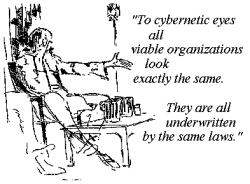
\includegraphics[max width=\textwidth]{sbmugs3_250x184}
\end{center}

This chapter contains a brief introduction to the fundamental ideas on which the Viable Systems Model (or VSM) is based.

The intention is to set the scene, to give you an overview, to sketch out the outline. So don't try and thoroughly understand it all. If you get an idea of how it developed, what it's about and why it's different from most other models, then it's done its job. Consider this chapter as a quick journey through a country you may decide to visit and study at a later date.

In some ways this is the most difficult task. The VSM is very different from anything else I've come across, and the tendency is to miss the whole point and re-interpret it as just another way of looking at the same old ideas of how organisations work.

The difference is that the VSM is a "whole systems" theory. Almost all other theories of organisation think in the billiard-balls mode of A leads to B leads to C, and therefore miss the essence of what's really going on. They forget that A, B and C are inextricably linked with a myriad other factors, and that for any model to work it must take all of this complexity into account.

The VSM is more in tune with other whole systems ideas like acupuncture, the Gaia hypothesis, most of modern physics and many aspects of Eastern religions. The trouble is that most of us see the world in different terms which have their perspectives set by the world-view of Newton and Descartes.

So the job is to provide you with a new way of thinking about organisations which is radically different from traditional, often hierarchical, models ...

The reward of this leap to new ways of thinking is the ability to think about organisations using a rich new language, and actually to be able to do something about problems which may be concerning you.

For this to happen, you have to learn to see the world through cybernetic eyes.

\begin{center}
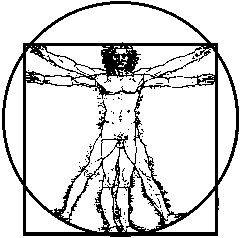
\includegraphics[max width=\textwidth]{v2man100}
\end{center}

\section*{2. The Approach}
During the 1950s Stafford Beer was working as a manager in British Steel and had become dissatisfied with traditional methods of organisation. Rather than attempt to modify what seemed to be a system of fundamentally flawed ideas he took a dramatically fresh approach. He began to study organisations which were obviously several light years ahead in the way they functioned. More specifically, he looked at the way the human brain organises the operation of the muscles and organs.

\textit{"We will seek the source of effective organisation in the cybernetics of natural processes - the brain itself."}

\textbf{We can study the extraordinary beauty of the human form, and base an organisational model on the methods used by the central and autonomic nervous systems to manage the workings of the organs and muscles.}

Beer's studies of the human form, the muscles and organs and all the various nervous systems were the inspiration for the Viable Systems Model.

It may be considered as a generalisation of the way that we all "manage" ourselves in response to a changing environment.

\begin{center}
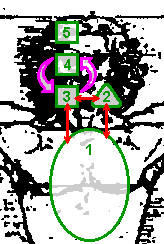
\includegraphics[max width=\textwidth]{1vsm4-1}
\end{center}

\subsection*{Generalisation - The Five Systems}
Beer's studies led him to view the human form as five interacting systems.

\begin{itemize}
  \item \textbf{SYSTEM 1}: All the muscles and organs. The parts that actually DO something. The basic activities of the system. The \textcolor{O}{\textbf{Operation}}.

  \item \textbf{SYSTEM 2}: The sympathetic nervous system which monitors the muscles and organs and ensures that their interaction are kept stable.

  \item \textbf{SYSTEM 3}: The Base Brain which oversees the entire complex of muscles and organs and optimises the internal environment.

  \item \textbf{SYSTEM 4}: The Mid Brain. The connection to the outside world through the senses. Future planning. Projections. Forecasting.

  \item \textbf{SYSTEM 5}: Higher brain functions. Formulation of Policy decisions. Identity.

\end{itemize}

\section*{3. The Three Elements \textcolor{E}{Environment}, \textcolor{O}{Operation}, and \textcolor{M}{Metasystem}}
Beer's first insight was to consider the human organism as three main interacting parts: the muscles \& organs, the nervous systems, and the external environment. Or a little more crudely, body, brain and environment.

These are generalised in the Viable Systems Model as follows:

\begin{tabular}{  p{0.1\textwidth}  p{0.9\textwidth} }
First	&	The \textcolor{O}{\textbf{Operation}}. The muscles and organs. The bits which do all the basic work. The primary activities.\\
\\
Second	&	The \textcolor{M}{\textbf{Metasystem}}. The brain and nervous systems. The parts which ensure that the various Operational units work together in an integrated, harmonious fashion. The job of the \textcolor{M}{\textbf{Metasystem}} is to hold the whole thing together.\\
\\
Third	&	The \textcolor{E}{\textbf{Environment}}. All those parts of the outside world which are of direct relevance to the system in focus.
\end{tabular}

\begin{center}
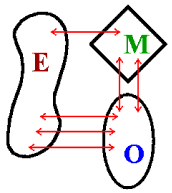
\includegraphics[max width=\textwidth]{vsmbasct}
\end{center}

\section*{Here is a basic VSM diagram}
The \textcolor{E}{\textbf{Environment}} is drawn as an amoeboid shape. The \textcolor{O}{\textbf{Operation}} and \textcolor{M}{\textbf{Metasystem}} are drawn as an ellipse and diamond respectively. (This is taken from Beer's conventions, although I have stretched his Operational circle into an ellipse.) The arrows indicate some of the many and various ways the three elements interact. Each arrow may have several aspects: information (by phone, computer, conversation), movement of trucks, people, money or goods.

{[}Note the approximation involved in drawing these three elements as separate. The \textcolor{E}{\textbf{Environment}} should really go all the way around both the \textcolor{O}{\textbf{Operation}} and its \textcolor{M}{\textbf{Metasystem}}. And the \textcolor{M}{\textbf{Metasystem}} should really be embedded in the \textcolor{O}{\textbf{Operation}}. The teasing apart is necessary to show the way the three elements interact .. {]}

\section*{4. The Three Elements as a Balanced Whole System}
Throughout the discussions which follow it is crucial to bear in mind that the VSM considers an organisation as a whole system which must be in balance with its environment.

This balance is the essence of VSM diagnosis. It's comparable to the approach taken by acupuncture which considers illness as an imbalance in the bodily functions diagnosed by an imbalance in the 12 pulses. Restore the balance - the illness goes away. And just as acupuncture will look at any imbalance between a patient and that patient's environment, so the VSM considers as fundamental the study of an organisation in its environment.

So, although it may be useful to take a limited view of some part of the VSM for a particular purpose, the emphasis will always be on the ecology of an organisation interacting with its environment.

This balanced whole-system approach resolves many of the dilemmas with which traditional models struggle. Should we centralise or decentralise?? Should we devolve power or appoint authoritarian managers??

All these questions will be dealt with as we build up the model. The design of the \textcolor{M}{\textbf{Metasystem}} depends upon the particular conditions within the \textcolor{O}{\textbf{Operation}}. They must be in balance. As the environment changes, the organisation must respond. This will usually require a change in the \textcolor{O}{\textbf{Operation}} to balance the environmental changes and then it's inevitable that the \textcolor{M}{\textbf{Metasystem}} will also have to adapt as it has to be in balance with its \textcolor{O}{\textbf{Operation}}.

All VSM diagnosis, analysis, and discussion is done in this way. The approach relies heavily on drawings and sketches which seem to be the appropriate way to represent a whole system. Quite often a few rough sketches will illuminate a problem which seems intractable when written as an essay.

\section*{5. The Five Systems (Physiological model)}
The Viable Systems Model is composed of the three elements: \textcolor{E}{\textbf{E}}, \textcolor{O}{\textbf{O}} and \textcolor{M}{\textbf{M}}. The \textcolor{O}{\textbf{O}} and \textcolor{M}{\textbf{M}} bits further subdivide into five interacting systems. They were originally derived from Beer's thinking about the "management" of the muscles by the brain and nervous systems.

Consider the following diagram of the central and autonomic nervous systems, shown interacting with both an external environment and (for this example) four muscles and organs.

\begin{center}
	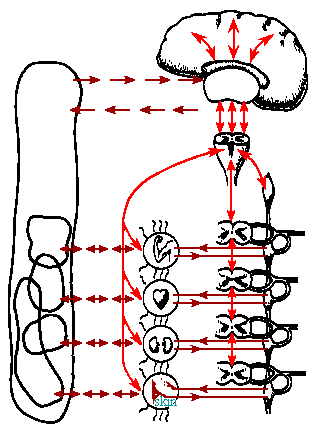
\includegraphics[max width=\textwidth]{pm5sys_}
\end{center}

{\renewcommand{\arraystretch}{1.5} %<- modify value to suit your needs
\begin{tabular}{ | p{0.14\textwidth} | p{0.76\textwidth} | }
	\hline
	\textbf{System 5} & The Cortex. Higher brain functions. \\
	\hline
	\textbf{System 4} & Diencephalon Input from senses, forward planning. \\
	\hline
	\textbf{System 3} & Base brain. Pons and medulla. Internal regulation. Optimisation. \\
	\hline
	\textbf{System 2} & The sympathetic nervous system. Its function is to stabilise the activity of muscles and organs. \\
	\hline
	\textbf{System 1} & Muscles, organs. Primary activities. \\
	\hline
\end{tabular}
}

In their (possibly over-)simplified form the five systems are as follows:


\section*{6. The Five Systems - Creating a Whole from the Parts}
I like to think of the five Systems in terms of what's needed in order to ensure that a number of parts come together to form an integrated whole system. The argument goes like this:

\begin{enumerate}
  \item First of all you need the working bits. This is System 1 (S1) which has previously been called the \textcolor{O}{\textbf{Operation}}. S1 is the bit which actually does something. It's the muscles, the engine room, the machines, the producers.

  \item Secondly you must ensure that there are ways of dealing with conflicting interests which are inevitable in the interactions which occur as the parts of S1 interact. Conflict resolution is the job of System 2. System 2 is also given the job of ensuring stability.

  \item Once the interactions of the System 1 units are rendered stable, it becomes essential to look at ways of \textit{optimising} these interactions. This is the job of System 3. System 3 works with an overview of the entire complex of interacting System 1 units and thinks "If this one does this and that one does that, then the whole thing will work more effectively." The extra efficiency is called synergy. System 3 is there to regulate System 1 - its function is optimisation.

  \item Once you have a stable, optimised set of Operational units, then you must ensure that it can survive in a changing environment. This is the job of System 4. System 4 looks at the outside world, considers what it sees, looks for threats and opportunities, and schemes. S4 is there to produce plans to ensure long term viability.

  \item And finally, the whole thing must function within some sort of overall context. Everyone must be pulling in the same direction. This is System 5's job. It provides the ground rules and the means of enforcing them to ensure that the system in complete. System 5 provides the ultimate authority.

\end{enumerate}

\textbf{The five systems develop into an extraordinarily powerful model of the way things work.}

**

The next step is to turn these ideas into a diagram.

**

\section*{7. The Five Systems - Graphical Representation}
\textbf{The result is shown below:}

\textbf{In VSM diagnosis you will re-think your organisation in terms of these five systems, and the most powerful approach is to visualise your understanding as a diagram something like the pictures on this page.}

\section*{8. The \textcolor{M}{\textbf{Metasystem}}: a little more detail}

\subsection*{The \textcolor{M}{\textbf{Metasystem}} is there to provide a service.}
In most traditional companies the Metasystemic jobs will be carried out by "higher management" - typically directors. In VSM terms they are only there to service the needs of the Operational parts of the organisation.

Compare this with the traditional view that the Operational parts are only there to carry out the orders of the Directors.

\section*{9. The \textcolor{O}{\textbf{Operation}}: a little more detail}
Whatever your organisation, the Operational part will be composed of sub-units. These are the Operational units. They may be people, or departments, or divisions, or separate companies.

This diagram shows the (large) Operational ellipse, inside which are three (smaller) Operational elements.


\section*{Review - The Form of the Viable Systems Model}
The model is recursive, that is the same principles of organisation \textit{recur} at all organisational levels, regardless of scale. This means that any Viable System is composed of smaller Viable Systems and is embedded in a larger Viable System.

\chapter{THE QUICK GUIDE TO THE VSM}\label{THE QUICK GUIDE TO THE VSM}
\noindent\fbox{
    \parbox{\textwidth}{%
        \centering
        \parbox{\textwidth - 6mm}{%%
            \vspace{3mm}
            In the following section, the entire VSM diagnosis is presented in brief.\\

            It will give you an overview of how the full diagnosis will proceed and of some of the diagrams which will be used.\\

            It will also enable those of you with some prior understanding and who have specific organisational problems to jump in at the sections that are most relevant.\\

            However, it should be stressed that until you have a reasonable understanding of the way in which the VSM looks at organisations, it may be difficult to grasp some of the concepts. If this proves to be the case, reading the Case Studies is perhaps the most accessible route to gaining the necessary background information.
            \vspace{3mm}
        }%%
    }%
}

\section*{Quick Guide: The Model}
The Viable Systems Model looks at an organisation interacting with its environment.

The organisation is viewed as two parts: \textbf{the Operation} which does all the basic work (production, distribution, earning the money) and the bits which provide a service to the Operation by ensuring the whole organisations works together in an integrated way (scheduling, accounts, strategic planning ...) These bits are called \textbf{the Metasystem}.

The following diagram illustrates the basic VSM.

\begin{longtable}[]{@{}
        >{\raggedright\arraybackslash}p{(\columnwidth - 2\tabcolsep) * \real{0.30}}
        >{\raggedright\arraybackslash}p{(\columnwidth - 2\tabcolsep) * \real{0.70}}@{}}
%    \endhead
    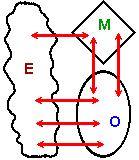
\includegraphics[width=\linewidth]{1vsm5}
    & \begin{minipage}[b]{\linewidth}\raggedright
        \begin{itemize}
            \item \textcolor{E}{\textbf{E}} represents the Environment
            \item \textcolor{O}{\textbf{O}} represents the Operation
            \item \textcolor{M}{\textbf{M}} represents the Metasystem
        \end{itemize}
    \vspace{\baselineskip}
    The arrows indicate the many and various ways that the three parts interact. Each arrow may have several aspects - it may be information, or trucks, a phone call or a delivery of steel ingots.
    \end{minipage} \\
\end{longtable}

The Operation will consist of a number of Operational units. These could be production units or teams of people doing various jobs.

The Metasystem can be divided in three main functions:

\begin{itemize}
  \item \textbf{The Internal Eye} - which looks at the entire collection of Operational units and deals with ways of getting them to work together in mutually beneficial ways, and with the resolution of conflicts. This is "Inside and Now".

  \item \textbf{The External Eye} - which looks at the external environment, assesses the threats and opportunities and makes plans to ensure the organisation can adapt to a changing environment. This is "Outside and Then".

  \item \textbf{Policy Systems} - which establish the ground rules which set the tone for the whole organisation. Policy rounds off the system. The policy systems must have ultimate control.

\end{itemize}

This is the basic model: The VSM sees any viable system as a collection of Operational elements which are held together by a Metasystem.

Both Operation and Metasystem must be in contact with, and interacting with, their environment.

The Operational units themselves must be viable, and thus can be looked at as smaller Viable Systems embedded in the larger system.

\section*{Quick Guide: The Model - Slightly Elaborated}

\begin{longtable}[]{@{}
        >{\raggedright\arraybackslash}p{(\columnwidth - 2\tabcolsep) * \real{0.60}}
        >{\raggedright\arraybackslash}p{(\columnwidth - 2\tabcolsep) * \real{0.40}}@{}}
    %    \endhead vsm-se5
    \raisebox{\normalbaselineskip-\height/2}{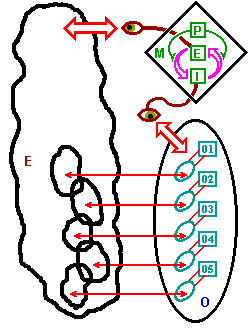
\includegraphics[width=\linewidth]{vsm-se5}}
    & \begin{minipage}[c]{\linewidth}\raggedright
       Note the three main parts - Operation, Environment and Metasystem.
       \vspace{\baselineskip}
       Note the Metasystem is shown with its internal and external eyes.
       \vspace{\baselineskip}
       Note the Operation is shown with five Operational units, all of which are smaller embedded Viable Systems
    \end{minipage} \\
\end{longtable}

\section*{Quick Guide: \href{https://vsmg.lrc.org.uk/3pd_5sys.html}{Preliminary Diagnosis}}
In the \href{https://vsmg.lrc.org.uk/3pd_5sys.html}{Preliminary Diagnosis} you look at your own organisation and examine the units which compose it. That is, you list the bits that do things, the co-ordination functions, the accounting and scheduling functions and so on.

You then draw a large VSM which will look something like the pictures on the previous pages to identify:

\begin{itemize}
  \item the Operational parts

  \item the parts which have inputs from the Internal Eye, and which deal with stability and optimisation of the Operational units.

  \item the parts which have inputs from the External Eye and which make long term plans in the light of Environmental information.

  \item the Policy Systems.

\end{itemize}

At the end of this process, you will have a large picture which gives a representation of your organisation in its totality.

This is the basic model from which the rest of the diagnosis will follow.

In some cases the \href{https://vsmg.lrc.org.uk/3pd_5sys.html}{Preliminary Diagnosis} will be the most useful aspect. You may find that your organisation has no way to carry out some of the functions which are vital for viability. Thus, you may decide to create new jobs to ensure these functions get perfomed. You may also find that some jobs don't seem to have anything to do with the Viable Systems. You may decide they are not necessary.

\section*{Quick Guide: \href{https://vsmg.lrc.org.uk/screen.php?page=4autonomy}{Designing Autonomy}}
It is essential to create the right conditions for all the Operational units to function with as much autonomy as possible.

Thus they will need

\begin{itemize}
  \item Individual Mission Statements.

  \item Budgets for the resources they need to carry out this Mission.

\end{itemize}

.-   An agreement that they can decide on their own internal development as long as they are working to the agreed Mission.

There will also have to be safeguards to ensure that the units cannot threaten the overall viability of the organisation of which they are a part.

Thus

\begin{itemize}
  \item They must be accountable and able to demonstrate they are working to the agreed plan.

  \item There must be pre-agreed intervention rules which means that autonomy is forfeit under certain conditions. The worst case scenario must be considered in advance.

\end{itemize}

\section*{Quick Guide: \href{https://vsmg.lrc.org.uk/5intbal.html}{Balancing the Internal Environment}}
By this stage you will have looked at the various parts of you organisation and decided how they map onto the VSM. You will also have considered the autonomy of the Operational units.

The Internal Environment consists of all the Operational units and those jobs which are dedicated to looking at them (The Internal Eye) and to ensuring that conflicts are resolved and that their performance is optimised.

Internal balance is concerned with these (Metasystemic) jobs and with ensuring that they have the capabilities to function properly. So for example, a committee which meets once every three months would be an absurd idea - most of these jobs need to be done on a continuous basis.

The approach to Internal balance is as follows:

\begin{itemize}
  \item Maximise autonomy so that the vast majority of problems are dealt with within the Operational units.

  \item Examine the exchange of goods and services between the Operational units, and see if improvements may be made.

  \item Examine the bits of the external environment peculiar to each Operational unit and see if changes can be made (perhaps they all use the same suppliers and thus benefit from joint buying).

  \item Optimise the allocation of resources to the Operational units. It may be possible to cut back in one unit and re-invest in another, thus creating synergy in the whole system.

  \item Examine the scheduling and co-ordination functions.

  \item Ensure that the information systems which inform the Metasystem of the goings on at the Operational level are well designed. How complete is the information? How up-to-date is it?

  \item And lastly, after all the above have been exhausted, it may be necessary to "beef up" the capabilities of the Metasystem in order to ensure it can discharge its functions of overseeing the Operational units. This is the usual way that traditional businesses operate, and in terms of both efficiency and of human working conditions should be seen as the very last alternative.

\end{itemize}

The essence of the internal balance is to view the Inside of your enterprise as a system of autonomous Operational elements, which need to be overseen (the Internal Eye) to look for ways of generating synergy.

The imposition of dictates from \textit{above} should only be used when the viability of the whole enterprise is at risk and not, as in traditional businesses, as the usual way of dealing with most problems.

\section*{Quick Guide: \href{https://vsmg.lrc.org.uk/6infsys.html}{Information Systems}}
The VSM requires thorough and up-to-date information systems.

The perfect information system would measure everything it needs to know continuously, so that a real-time model of the goings on within any part of the enterprise may be maintained.

The compromise between this and the usual management information which is weeks or months out of date is the use of daily performance indicators.

These measure whatever is seen as important within each Operational units (productivity, morale, wastage, sales, breakages ...) at the end of each day. The figures are then plotted onto a time series so that the trends may be assessed.

\textbf{The essence of the VSM approach to information is that you only need to know if something changes.} If everything is going as normal, you can leave it alone. However as soon as something changes (dramatic fall in productivity) it's essential you are notified immediately.

Thus:

\begin{itemize}
  \item Huge printouts of standard information which say "\textit{nothing much has changed}" are useless.

  \item Immediate alerting signals which say "\textit{something dramatic has happened}" are essential.

\end{itemize}

These signals, which are called \textbf{algedonics}, are the basis of information handling in the VSM. They can be designed to provide Operational units with the information they need to learn and adapt to environmental changes, to define clear limits to autonomy, to guarantee that each Operational unit is working as an integrated part of the whole-system and so on.

The design of these information systems is crucial to the effective operation of your enterprise, and can be used as an alternative to authority.

\section*{Quick Guide: \href{https://vsmg.lrc.org.uk/7envtbal.html}{Balance with the Environment}}
The External Eye maintains contact with the relevant parts of the external environment, and enables the future planning systems to develop strategies for adapting to change in the market, or to new technology, or whatever.

Again, the various parts must be balanced:

\begin{itemize}
  \item The future planning system must have the capabilities to examine and find the relevant information.

  \item It must be capable of planning and simulating various options.

  \item It must be aware of the capabilities of the Operational units, and develop any strategies within this context.

  \item It must be able to agree and implement its plans through the connections to the Operational units.

  \item It must function within policy guidelines.

\end{itemize}

\section*{Quick Guide: \href{https://vsmg.lrc.org.uk/8psysdes.html}{Policy Systems}}
The policy systems oversee the entire organisation. They constitute the ultimate authority. Clearly they must be designed with great care.

For a co-operative it is crucial that everyone is involved in policy decisions and this usually involves a meeting of all members.

However, the practicalities of this need to be addressed. How often can the entire membership meet? How effective are big meetings? The answer to the question of how you involve all members in policy decisions and how you ensure that everyone has to work within these ground rules is perhaps one of the biggest questions for any Social Economy enterprise, and will determine the extent to which it may describe itself as democratic.

\section*{Quick Guide: Basic Vocabulary}
This Quick Guide to how the VSM looks at organisations and how it ensures the various parts are balanced has introduced most of the basic vocabulary.

\begin{itemize}
  \item Autonomous Operational units.

  \item Metasystem - concerned with ensuring the Operational units hang together or cohere into a single integrated organisation.

  \item Synergy - the added efficiency which comes from working together in a co-operative fashion.

  \item Daily Performance Indicators - which measure the goings on within each Operational unit.

  \item Algedonics - signals which are generated to say "Look out .. something unusual has occurred"

\end{itemize}

From now on, the manual will assume you understand these terms.

It will also use the five systems to describe the various functions within the organisation.

\chapter{CASE STUDIES}\label{CASE STUDIES}
This Section contains three case studies which illustrate the application of the VSM to co-operatives of different sizes.

The first involves a small co-operative of 5 people, and clarifies the mechanisms whereby a small unstructured group can demonstrate viability.

The second describes a study of a medium size group of 35 people who were experiencing organisational difficulties, the conclusions that were reached using the VSM, and what happened when they were put into practice.

The third involves the (huge) Mondragon co-operatives in an attempt to see if the VSM can throw any light on their astonishing success.

\section*{Case Study 1: HEBDEN WATER MILLING COLLECTIVE 1985}
I began with HWMC because at that time it was the enterprise that I knew most about.

I had been involved in setting it up in 1980, and had seen it grow and prosper in its first five years without any formal structure.

The task I had set myself was to see if the VSM could describe the mechanisms which enable a small loose co-operative to function in an undeniably viable fashion.

Or ... if the VSM had said "this just can't be viable as you don't have a System X, and that's a fundamental of all viable systems" ... I would have had serious doubts about its usefulness to co-operatives.

\section*{Background}
HWMC is a small co-operative that was formed in 1980 to blend and package a large range of wholefoods using fairly complicated machinery.

For the period 1980 - 1985, HWMC was successful both in its financial performance and in the working environment it provided for its members. The production processes became extremely efficient, crises were dealt with effectively, challenges were met and discharged, relations between the members were excellent, profits were good, and in general the system worked beautifully.

All decisions were made by consensus, and weekly meetings (when necessary) usually lasted about ten minutes.

Working procedures evolved during the day: after a 30 second planning session ("Let's do the Basmati rice first"), everyone would work around each other, without formal planning, and the days production would proceed. The process is much more in sympathy with the operation of a Jazz band or a football team: basic rules and constraints are understood, but the specific actions performed by the participants are dictated by the conditions of the moment.

\[As an aside, I should mention that working in this way has been one of the most satisfying experiences that I have had, and goes some way to explain why co-operatives are full of graduates doing apparently boring manual jobs.\]

\section*{Preliminary Diagnosis}
The initial diagnosis began with the five members positioned as the Operational units. The Metasystem was also composed of all five members, but in a different role: when the work was being done they were \textbf{Operation}, when planning was necessary they articulated the \textbf{Metasystem}. The fundamental co-operative principle of \textbf{self-management} means that there is no clear division in the roles of people working within the group: everyone is obliged to be both "manager" and "worker."

Generally, as the diagnosis proceeded it became obvious that as a function was identified (for example a System 2 stability function whereby the available worker-power was effectively allocated to the various tasks) the same principle was in operation: all members identified the need to articulate a particular Metasystemic function - often without verbal acknowledgement - and shifted into the appropriate mode to deal with the situation.

In many cases, the Metasystemic functions could be done while the Operational work was proceeding (we're nearly at the end of this run ... has anyone got the next one ready?) whereas other discussions required the temporary suspension of manual work, or in unusually complicated situations a few hours put aside to generate plans and strategies.

\section*{The Mechanics of Viability at HWMC}
\begin{itemize}
  \item Most Metasystemic activity (systems 2 and 3) is present continuously.

  \item Work proceeds as described above. As long as nothing unexpected occurs very little Metasystemic activity is needed. Most Metasystemic activity (systems 2 and 3) is present continuously.

  \item The \textbf{model of the Operation}, located in System 3 and crucial to viability, is continuously being upgraded in the minds of the members. Thus the System 3 model is up to date and virtually complete. (It even knows if someone changes his shirt.)

  \item \textbf{Instabilities} in the production techniques are usually dealt with immediately for two reasons: firstly, all members share a compatible System 3 model; and secondly, the performance of the Operational elements is based on co-operation and not competition.

\end{itemize}

.-   The Metasystem is alerted immediately it is needed: any crisis (for example a sudden large demand for muesli, or a machinery breakdown) suspends the Operational activity briefly and the Metasystem springs into action - that is everyone goes into a huddle; \["Can we cope?" "I can do a couple of hours after work." "Jack is free tomorrow lets get him in."\] and so on.

\begin{itemize}
  \item The operation of System 4 is firmly based on the System 3 model, and as long as long as everyone has their wits about them , the whole thing works very effectively.
\end{itemize}

\section*{Conditions for Viability in a Small Group}
Having experienced this process for a number of years, it is apparent that three conditions are necessary for viability. They are as follows:

\begin{enumerate}
  \item Everyone must be capable of, and involved in, both Operational and Metasystemic functions: if this is not the case, the capabilities of the Metasystem will not be sufficient to deal with the Operation.

  \item Efforts must be made to ensure the completeness and availability of the System 3 model. In HWMC, everyone was present most of the time, so there was no problem.

  \item The mechanics of viability are completely dependant on \textbf{thorough discussion}. Effective discussion is essential in the generation of the System 3 model, the workings of the necessary interaction between System 3 and System 4, and the successful discharge of all Metasystemic functions.

\end{enumerate}

Usually, in a group of four or five people, there is no problem in satisfying these three prerequisites, and viability is relatively straightforward provided that everyone works as a team for the majority of the time and the need for all the Metasystemic functions, especially future planning, is recognised.

There would seem to be nothing to prevent a non-structured organisation of this kind working Viably.

\section*{The Collapse of Viability in a Small Co-operative}
The weakness of the kind of structure exhibited by HWMC is that viability is entirely dependant on the people involved. There is no formal structure to ensure effective viability. Consequently it is not uncommon for the group to degenerate into a non-viable form.

\section*{1. Problems with the Metasystem}
There are many ways in which the capabilities of the Metasystem can be affected. For example, if a new member lacks confidence he may not feel able to enter into a Metasystemic function, as this may be seen to be the province of more experienced members. Thus vital information may not be forthcoming in a System 3 meeting.

Exactly the same problem may emerge if the "old hands", by their attitudes, discourage new members from becoming involved at all levels.

There also seems to be a potential danger that in a co-operative which involves much concentration at the Operational level (say a co-operative of computer programmers) very little brain power will be left to deal with Metasystemic issues. In this case it may be necessary to appoint a member to deal mainly with Metasystemic issues, and in this case a different organisational structure will be needed.

A further problem could emerge in a period of continuous crisis when the Metasystemic functions need such a large amount of the time that the Operational functions are neglected (that is, no production gets done). This could be overcome by extending production time, but again the division of the Operational and Metasystemic functions is a possible solution.

\section*{2. Problems with the System 3 Model}
One of the more common complaints from people who deal regularly with co-operatives is that essential information is not available when it's needed.

This may be caused by movement of members (the relevant information was given to Jill who is out driving today ...), by feelings of unimportance (Jack doesn't think he's valued enough to make a contribution, although he may know the crucial element ...), and so on.

Recognition of the absolute necessity of the System 3 model for viability may be one of the more important contributions of VSM theory to co-ops. It may also avoid the usual knee-jerk reaction to the lack of the System 3 model which is: appoint a manager. Although this would allow a complete System 3 model to be generated (the Manager would act as a reference point for everyone and would thus accumulate the necessary information), other ways may be more appropriate such as a computer model or a large blackboard or magnetic shapes on a sheet of metal.

\section*{Summary: Conditions for Viability}
A small group may demonstrate viability as long as:

\begin{enumerate}
  \item All members are capable of both Operational and Metasystemic functions
(i.e. they can do the basic work and discuss optimisation, policy, future plans ...)

  \item All members are present all the time. Metasystemic functions need to refer to a real-time complete model of the Operation. If some people are not present, and they have the crucial information needed for a decision, then that decision will be made in ignorance.

  \item All decisions must be based upon thorough discussion by all members.

  \item All Metasystemic functions must be recognised and performed.

  \item The need to keep an eye on the external environment must be recognised, and this information should be used to generate plans to adapt to the future.

\end{enumerate}

\section*{Conclusion}
Having worked in this kind of co-operative for many years and experienced just how efficient and rewarding it can be, it is clear from the VSM analysis that two conclusions may be made:

\begin{enumerate}
  \item This kind of unstructured small group is able to demonstrate viability in the terms used in VSM studies.

  \item This viability is fragile.

\end{enumerate}

The first three conditions for viability are not impossible to meet, but viability can collapse as membership changes, members' personalities clash, some people feel they can take on Metasystemic jobs without consultation, and so on. Condition 2 is obviously difficult due to holidays and sickness, and thus the Metasystem will occasionally have to cope with an incomplete model.

Two recommendations may be offered

\begin{itemize}
  \item That daily performance indicators are measured and displayed in meeting places. This will complement the model of the Operation which accumulates during work and discussions, and if viability does begin to collapse, there will be immediate alerting signals.

  \item That there are regular slots on the agenda to discuss internal optimisation and future plans to ensure these two conditions for viability are met.

\end{itemize}

\section*{Case Study 2: TRIANGLE WHOLEFOODS}
This Case Study examines the problems which had emerged at Triangle Wholefoods (trading as \href{http://www.suma.co.uk/}{Suma}) as it grew from a small group to become one of the largest co-operatives in the UK.

It is clear that as numbers grow, meetings become more and more difficult. There are various ways of looking at this but the basic principle is clear: small meetings work - large ones don't.

The exact numbers vary with the type of organisation but in general under 11 is easy, between 11 and 20 is difficult but manageable, above 20 is just unworkable without very small agendas, lots of preparation and rigid control from the chair.

Suma was attempting to perform all its management through a single weekly meeting of all members, and it clearly was not working.

The task of the VSM was to design an effective organisation without resorting to managers, or authority/obedience techniques.

\textbf{Note:}

The material in this section was written in 1986, with additional material added in 1991.

\section*{Background}
TRIANGLE WHOLEFOODS, trading as Suma, began in the mid seventies with a loan of £4,000 and was supported by the five wholefood retail co-operatives in the north of England who agreed to buy everything they could through Suma. This gave Suma a guaranteed minimum turnover.

Over the following three years, the number of wholefood co-operative shops in the region grew enormously to around 60 by 1980, and Suma prospered accordingly.
Since that time the co-operatives have become a less and less important part of Suma's turnover: there are now around 2,500 customers.

Currently (1998) Suma operates in a 60,000 sq. ft. warehouse in Halifax, offers a range of about 7,000 products (3,000 in 1991, 5,000 in 1995), and distributes nationally with a growing number of exports. There is some in-house pre-packing and bottling. Recent years have seen the introduction of several own-label products and the growth of environmentally sound products.

Suma has always attempted to base its working practices upon the needs of its members - job rotation and flexible working conditions are common. Equal numbers of men and women has generally been achieved.

At the time I was applying these ideas, SUMA, consisted of about 35 workers with a turnover in the region of 6 million ECU.

Some departments had evolved (transport, manufacturing, warehouse), there were two committees which considered financial and personnel matters, and the entire membership was supposed to meet for the weekly Management Meeting every Wednesday afternoon. This meeting was the \textbf{only} recognised decision making body within Suma, and as such had to deal with all departmental issues as well as Suma policy. It also had to ratify the recommendations from the committees.

The problem which had triggered the VSM study was an almost universal recognition that the Wednesday meetings were not working. As the size increased, agendas were getting longer and longer, less and less was getting dealt with, arguments were common, and many people didn't like to have departmental matters voted on by a large group, most of whom had no direct experience of the issues.

Consequently, members began to avoid the meetings, some decisions were taken unconstitutionally outside the meetings ("but someone had to decide and the Wednesday meetings are useless") and it was realised something had to be done.

\section*{DIAGNOSIS:}
\begin{center}
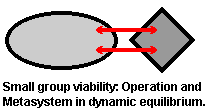
\includegraphics[max width=\textwidth]{2cs2-f1}
\end{center}

Suma had started as a small co-operative in which the Operation and Metasystem were balanced, as described in the study on HWMC. This is illustrated by the diagram shown on the right.

As the numbers grew and the limits to this kind of viability were passed, problems began to emerge.

The structure was still basically the same: the Operation was conceived as a single entity and the once a week all-member meeting was seen as the only Metasystem.

\begin{center}
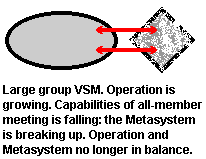
\includegraphics[max width=\textwidth]{2cs2-f2}
\end{center}

The complexity of the Operation was growing explosively in terms of new customers, new products, more services, and more manufacturing, and consequently viability required that the Metasystemic functions had to grow to cope. Some attempts were made to do this (the Finance and Personnel committees) but as the dominant Metasystemic body was the all-member meeting - and as numbers grew beyond 20 this became practically unworkable - the capabilities of the Metasystem were actually decreasing.

In order to deal with this, departments had been set up to deal with the Warehouse, Transport, Manufacturing, Order-picking and so on, but they were still obliged to make all important decisions through the all-member meeting. Thus, they did not have the autonomy they needed to deal with their own problems.

\section*{DIAGNOSIS OF SUMA 1986 (Structure only)}
The diagram opposite shows a VSM with five Operational units (\textbf{O1} to \textbf{O5}). The environment is not shown as the current discussion is limited to the internal structure.

\section*{METASYSTEM}
\begin{center}
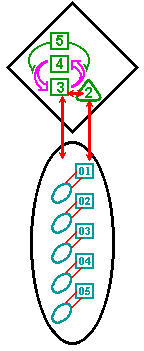
\includegraphics[max width=\textwidth]{2cs2-f3}
\end{center}

\textbf{System 5 (Policy)}

All member meeting. Doesn't work due to number of members.

\textbf{System 4 (Future planning)}

Almost completely absent. Performed by \textit{ad hoc} groups. No 5 year plans. No marketing direction. No formal market research.

System 3 (Synergy)

Some attempts by finance and personnel committees. Hampered by dynamics of all-member meeting. Needs continuous implementation. Some personnel optimisation through the weekly Rota.

\textbf{System 2 (Stability)}

Co-operative ethos and wages policy makes conflict of interests unlikely. Cash flow controlled. Weekly Rota. Fairly robust.

\textbf{System 1 (OPERATION)}

The 5 Operational units illustrated are the Warehouse, Transport, Order Picking, Manufacturing, and Order Taking.

In all cases the problem is the same: the ability to organise the departments effectively is frustrated by the lack of autonomy. The departments, charged with their own internal organisation do not have the freedom they need to work effectively.

\section*{CONCLUSIONS:}
\begin{enumerate}
  \item THE POLICY PROCEDURES NEED TO BE RESTRUCTURED

  \item FUTURE PLANNING AND SYNERGY SYSTEMS NEEDED

  \item STABILITY SYSTEMS NEED TO BE CONSOLIDATED

  \item DEPARTMENTS NEED TO BE MADE AUTONOMOUS WITHIN COHESIVE LIMITS

\end{enumerate}

\section*{THE DOUGHNUT PROPOSALS}
From the above considerations, it became clear that Suma had to rethink itself into autonomous departments. It was equally clear that these departments needed to cohere into a single harmonious organisation. In April 87, four of us produced the Doughnut Proposals which involved local decision making, new functions to articulate the all-Suma Metasystem, and the replacement of the Wednesday meeting with a system of small meetings ("Sectors") which sent delegates to the articulation of System 5 which eventually became known as the "Hub".

The Doughnut proposals involved two VSM fundamentals:

\begin{itemize}
  \item The Operational units must be given as much autonomy (freedom) as possible and the only restrictions involves system cohesion. OR ... you can't give the Operational units complete autonomy as the organisation may fly apart.

  \item Appropriate information gathering and filtration. Whereas the Orwellian view is that information is of use in limiting freedom, the VSM is based upon the principle that information can give an individual the information he needs to organise himself, and thus underwrites individual liberty. The better the information system, the more freedom an individual can have.

\end{itemize}

\section*{IMPLEMENTATION}

\section*{The First 9 Months}
After weeks of debate and lobbying Suma accepted the Doughnut proposals by 25 votes out of the then 29 full members. However, rather than a smooth transition to the structures we proposed, Suma accepted that Things Had To Change and proceeded to try a succession of ideas, some based on the Doughnut proposals, some on the original structures and others on a combination of the two. It was all very unsettling.

One of the problems was that Suma had decided not to drop the old system and go for autonomous departments, but to run the two systems in tandem for a transitional period. While this seemed quite sensible, the old committees refused to relinquish any of their powers and it became clear that they were actually \textbf{preventing} the new structures from becoming effective. It also meant that meetings began to proliferate, as several groups thought it was their job to discuss a particular issue.

After about 6 months of this, the four of us who had produced the original proposals re-convened and produced a further 7 proposals aimed at resolving the situation. Most of these were accepted and implemented immediately; the result still forms the basis of Suma's organisational structure.

\section*{PROPOSALS AND OUTCOMES}
The original proposals were seen as something of a leap in the dark, and most members only accepted them as it was clear \textbf{something} had to be done, and that hierarchical solutions were not acceptable politically.

In the following pages I will take the original proposals (as they were written in 1987), recount what happened in the first few months, and how they developed into our current (1991) structure.

It should be remembered that Suma has been subjected to many other influences over the last five years, and that the Doughnut proposals cannot take the credit for all that has transpired.

The proposals describe the Operational elements as "Segments", the name was later changed to "Sectors".

Similarly the "inter-segment committee" became known as the "Hub".

\section*{PROPOSAL 1: FORMATION OF SEGMENTS}
**

"We propose that Suma formally divides into small groups of around 7 to 10 people.

Each group would work as a close-knit team with responsibility for a particular area of Suma's Operation.

Each group would be given as much autonomy as possible within Suma to deal with its own problems and pursue its own internal development."

**

The Outcome:

Initially very little changed. The theory was that departments could ask for more autonomy as they needed it. During the first year departmental budgets were set up, and thereafter departments had financial autonomy within these limits. And gradually they became more autonomous.

We had originally thought that some small departments might group together into new Operational units - the Segments - but this didn't happen. The original departments stuck to their original form.

Currently most departmental decisions are made internally: all departmental expenditure, and most personnel matters, are dealt with autonomously. It is now recognised that most jobs are fairly specialised and that it would be foolish to have everyone involved in everyone else's business.

Most of the basic conditions for autonomous departments have now become established.

Recent examples are

\begin{enumerate}
  \item The warehouse buys racking and fork trucks from within its budgets.

  \item The office instituted a new system of computerised order taking without reference to the rest of the co-operative.

\end{enumerate}

\section*{PROPOSAL 2: LIMITS TO AUTONOMY}

\section*{PROPOSAL 3: CO-ORDINATION OF SEGMENTS}
**

"Some new functions will be needed to ensure the segments work in a positive way.

We propose a new committee which is formed specifically to ensure the segments work together co-operatively.

This Inter-Segment Committee would consist of one delegate from each segment and would meet once a week to deal with problems between the segments and to suggest ways of improving over-all performance.

We see this committee eventually replacing both the F.C. and the P.C. and forming the basis on which the segments work together."

**

The proposed new meeting, which became known as the Hub, began to meet just as we had intended. However, we had expected it to deal mainly with inter-departmental (nuts and bolts) issues whereas the vast majority of Hub agenda was taken up with all-Suma policy. Initially some internal departmental issues were taken to the Hub, but as the departments were supposed to be autonomous, the Hub referred them back.

\textbf{Essentially the Hub took over from the all-member meeting except for internal departmental issues.}

Currently, the system works as follows:

Once a week everyone who is interested meets in Sectors: groups of about 10 people. They discuss all the issues in the Sector Pack which begins with the minutes from the previous week's meetings, any minutes from other meetings which are relevant, proposals from members and anything else which requires the scrutiny of the whole co-op.

Sector minutes are kept carefully and each meeting sends one delegate to the Hub. The various delegates read the relevant minutes and then make a decision based on the majority view within the co-op. Usually this is straightforward, but some issues are very complex and each Sector may come to a different conclusion. The Hub will usually summarise these views, clarify the lack of consensus and send the issue back for further discussion. Sometimes it becomes clear that a subject requires further thought and as such is referred to a committee. Eventually most Sectors come to similar conclusions and the Hub formalises the decision.

Most decisions are made quickly, a few require two or three trips around the Hub/Sector system, and very occasionally it becomes necessary to call a General Meeting of all members to resolve a particularly difficult issue.

There are two further safeguards on this system:

\begin{itemize}
  \item No Hub decision becomes law until a week after it is made. In this week anyone who may have missed the meeting, can ask for it to be re-discussed in the light of new information.

  \item Any five members can call a General Meeting at any time to discuss an issue they believe has been dealt with badly.

\end{itemize}

These safeguards were introduced to ensure that the Hub did not develop into a managerial elite. In practice they are almost never used: but everyone knows they are there.

\section*{PROPOSAL 4: ACCOUNTABILITY \& COMMUNICATION}
**

"Some way must be found to measure what's going on in each segment so that information is available to co-ordinate and make decisions, and so that segmental Autonomy can be given clear limits.

We propose the use of the system of indices, together with the \textit{Cyberfilter} program to extract important information.

This system puts the responsibility for segmental development on the segments themselves. The information from the system is an immediate representation of what's going on."

**

\textbf{\[Note: The "Cyberfilter" referred to here was a specific implementation of a change-detection system, using the Harrison-Stevens Bayesian forecasting algorithm. This was just one of many potential approaches to detecting incipient instabilities, but one which found favour in mid 1970s VSM applications.\]}

This proposal was without doubt the most radical: we were proposing to move to real-time regulation and to use cybernetic filtration of information in order to generate algedonics. (All of this is described in more detail in Section 6).

There are several aspects to this system:

\begin{itemize}
  \item It provides a complete and current record of all important goings on within each department.

  \item It provides the feedback necessary to enable the members within each department to control their performance.

  \item It gives a structure to Autonomy. Each department was to have an agreed amount of time to solve its problems once an indicator moved outside the acceptable limits.

\end{itemize}

We ran some tests on the systems using the manufacturing department. The indicators measured daily were productivity, machine usage, wastage and happiness. Between them these indicators gave a complete picture of the goings on within this department.

Although the calculation of indicators only took up a few minutes at the end of each day, the system was never formally adopted by the co-op. They were seen to be too difficult to use and at the time there was no interest in making departments accountable.

Over the last five years I have used indicators in the pre-packing department to measure productivity, wastage and out-of-stocks, and still find the system as useful as it seemed originally. However, they are only used within the department - there is still no overall system to ensure the departments are accountable. The only formal system involves the buyers: every week the sales loss through out-of-stocks is measured and plotted as a time series. This is then put in the Sector packs so that everyone knows what is happening. If this indicator began to rise alarmingly, the whole co-operative would know.

There are several other informal performance indicators including daily tonnage, daily sales, the number of lines of orders taken by the sales office, and so on. However the integration of these into formal reporting systems, specific limits to autonomy and overall accountability has never been undertaken.

\section*{PROPOSAL 5: FUTURE PLANNING}
**

"Decision making has already been transformed in the organisational structure proposed so far:

\begin{itemize}
  \item Day by day decisions will be made within close-knit groups and will not clutter up the agenda on a General Meeting.

  \item Co-ordination decisions will be made at weekly meetings of delegates."

\end{itemize}

"This leaves the issue of decisions concerning the outside world as it affects Suma, and long term strategic decisions."

"We propose a new function within Suma to deal with these issues which:

\begin{itemize}
  \item Finds out what's happening in the outside world and its likely effect on Suma. Where appropriate this information can be passed on to the relevant segment.

  \item Considers this information in conjunction with Suma's internal capabilities.

  \item Comes up with FUTURE STRATEGIES about where Suma could be going, marketing, organisation, new products etc.

  \item Thoroughly researches a number of options.

  \item Presents their findings and recommendations to a General Meeting of all members, who make a decision."

\end{itemize}

**

For months, nothing happened whatsoever.

Most of Suma's energies were taken up in dealing with the internal problems and the need for a Futures function was seen as a very low priority.

The issues raised its head again in 1988 after the Hub/Sector system had become established, and this time was pushed hard by the Marketing Department who had recognised the need for a long term marketing strategy, and needed a Business Plan within which to work.

Three members were elected and given the job of researching possible future strategies. A vast number of options were looked at, but nothing actually happened. No proposals were produced.

Currently we have hired consultants to provide us with a 5 year business plan and they have recommended we set up a "Business Plan" group to administer the plan.

However, it would appear that the mechanisms that are being proposed involve analysis of variance and will further strengthen the System 3 (internal control) function. They will not in fact address the need for a System 4 as suggested in these proposals.

\section*{PROPOSAL 6: QUARTERLY GENERAL MEETINGS}
**

"As the general meeting would only be needed to discuss major policy decisions, they would only have to happen every three months.

In exceptional circumstances they may be needed more regularly, and extra-ordinary GMs could be called by the Intra-Segment Committee at any time."

**

As the Hub/Sector system became established it dealt with Policy matters so successfully that General Meetings (of the entire workforce) became almost unnecessary.

Very rarely an issue proves to be too complicated to discuss in separate meetings, and it becomes essential to assemble all the arguments with all the members. This has only happened twice in the last few years.

The new system also allows any 5 members to call an Emergency General Meeting for any reason whatsoever. This has been threatened a few times, but so far it has resulted in the re-discussion of the subject through the Sectors.

Generally it is now accepted that General Meetings are unnecessary except in exceptional circumstances.

\section*{REVIEW OF ORIGINAL DOUGHNUT PROPOSALS}
It's clear that the concept of autonomous departments and the need for a Metasystem to cohere them has worked for Suma.

It's also clear that some of the original details just didn't happen (for example the combination of departments into Segments) and that some of our ideas were re-worked by the co-operative. (For example, the Hub/Sector system was adopted to work almost exclusively with Policy and not with the practicalities of departmental optimisation).

Five years later, it still seems that the basic ideas are sound although the way that we originally interpreted them was far from perfect.

The aspect which we had completely misjudged was the actual implementation. After the acceptance of the proposals, I expected a fairly smooth transition with the support of most of the co-operative.

The reality was that Suma generated a series of excuses for putting off the actual implementation (it's summer so lots of people are on holiday. Now we're getting ready for the Christmas rush ... ) and the actual process had to be pushed very actively.

The details of the period of implementation are not of direct relevance to this case study, although it should be noted that embarking on a programme of radical change in any organisation can be an extremely hazardous occupation.

\section*{FURTHER DEVELOPMENTS}
During the initial implementation, there was a particularly chaotic period during which the Hub self destructed and divested its powers into the Personnel and Finance committees. As these bodies were \textit{a)} designed to deal with a non autonomous Suma, and \textit{b)} able to deal only with specific issues and thus not capable of taking the overall, synoptic view, the situation was unworkable.

In this context, three of the four original Doughnut members met and made a further set of 7 proposals:

**

"If Suma decides to make another attempt at the Doughnut, it's essential to make a much more concerted effort to establish the new system: the old working methods have proved to be more deeply entrenched than we imagined."

"Our proposals are as follows:

**

The crucial elements of the November 87 proposals were accepted and implemented, and still form the basis on which we organise ourselves.

\section*{SUMMARY and ASSESSMENT}
It is clear that the major parts of the System are now in place.

\textbf{System 1: Operation.}

The departments are autonomous within limits set by financial and personnel budgets.

\textbf{System 2: Stability.}

Co-operative working practices continue to keep inter-departmental problems to a minimum. There is now better cash flow control and a recent system of stock control. Stability is further helped by improved co-operative information systems (e.g. the weekly business info).

\textbf{System 3: Optimisation.}

The Finance and Personnel officers \& their committees deal with allocation of resources, and a weekly Rota looks at the best ways of placing personnel. Occasionally committees are set up to deal specifically with optimisation: recently three members were given the task of looking at our job requirements and fitting the best people to each job.

\textbf{System 4: Future Planning.}

The Futures Committee exists although it is presently not functioning in the pro-active way which the VSM sees as fundamental. The eventual outcome is not clear at this point.

\textbf{System 5: Policy}

Suma continues to involve all members in all policy matters on a continuous basis and this has to remain one of the rocks on which the co-operative is organised.

The link between System 1 and System 5 is crucial.

\textbf{The Doughnut proposals began a process of re-organisation which is still in progress. It would be misleading to say that all the proposals were accepted and implemented: it is more accurate to say that we pushed Suma in a particular direction and that the final outcome is the result of the way Suma adapted to that push.}

I view the application generally as a success.

In 1986, the weekly General Meeting had become the most commonly perceived problem. In a recent survey the Hub/Sector system was not even mentioned in the members' list of dissatisfactions. Financially Suma has performed well during the last few years, and seems to be riding out the present recession. The enormous increase in Operational variety over the last three years make it reasonably certain that the pre-VSM structures would not have been able to cope. Had the Autonomy Proposals not been accepted, the only other alternative would have been democratically appointed managers, the introduction of authority-obedience procedures, and consequently the loss of perhaps the most important element of the co-op's success - the self management of most of its members.

It also seems reasonably certain that without VSM theory, the proposals from the Autonomy Group would have been unable to answer many of the criticisms which were levelled at it. The VSM enabled us to present a complete and thorough package, and thus played a crucial role in the development of the co-op.

\section*{Further Enhancements (April 1991)}
There are several areas in which the structure of Suma could still be improved.

\begin{enumerate}
  \item \textbf{Policy}

The Hub/Sector System works wonderfully in keeping everyone involved in policy, However sometimes issues arise which are too complex to discuss in separate meetings, and often a conclusion is avoided. It would seem sensible to make quarterly meetings of all members compulsory in order to resolve these issues, and for everyone to hear from everyone else once in a while.

  \item \textbf{Departmental Optimisation}

The optimisation function has never been formalised. We had originally intended that the "Inter-Segment Group" did the nuts and bolts, how-do-we-work-more-effectively, System 3 stuff, but the Hub developed into a System 5 policy body.

The recent proposal from the business consultants to have a monthly meeting of departmental co-ordinators and to optimise departmental interactions should discharge System 3 effectively, but much depends on the methods they employ for accountability.

  \item \textbf{Performance Indicators}

The performance indicators still look like an extremely efficient means of looking at accountability, of formalising departmental feedback and of putting limits on autonomy. However, they are still so different from usual methods of dealing with organisational information that people are loath to adopt them.

  \item \textbf{Autonomy.}

Departmental autonomy has now become almost complete: the only improvement could be better liaison between the Personnel Officer and Departmental co-ordinators.

Currently some departments are occasionally allocated unsuitable people due to problems with the Rota as a whole.

However, this is a minor quibble - the balance between departmental needs and overall personnel is generally handled well.

  \item \textbf{Futures}

There is still a desperate need for a System 4: someone to keep informed of the markets, external threats and opportunities, and to produce strategies aimed at ensuring Suma can adapt to future eventualities. This must be on a continuous basis, it's clear that System 4 cannot be discharged by an occasional planning meeting.

For an organisation of Suma's size it seems essential to appoint at least one person to do all the System 4 stuff continuously.

\end{enumerate}

\section*{Case Study 3: ONE MONDRAGON CO-OPERATIVE}
This case study is a diagnosis.

I visited \href{https://www.mondragon-corporation.com/en/}{Mondragon} in February 1991 in order to look at the way they handle federations of co-operatives. However, much of what I learned about the organisation of a single enterprise was of such relevance to the use of the VSM, that I felt bound to include it in these case studies.

Many of the conclusions I made concerning Suma have been reached by the Mondragon co-ops, presumably by entirely different routes.

And in many cases they have adopted practical solutions which fit in exactly with some of my more theoretical proposals.

\section*{BACKGROUND}
My visit to Mondragon was primarily to study the way that they manage to get 173 different co-operatives to collaborate. However, the structure of their manufacturing plants has been changing recently, and these changes were of direct relevance to the conclusions I have been coming to through VSM diagnosis.

\href{https://www.mondragon-corporation.com/en/}{Mondragon} are the most successful group of co-operatives that I know, and during the visit I made in February 1991 I was continuously impressed by their commitment to both co-operative ideals and to state-of-the art production techniques. All the factories are full of computer controlled machine tools and robots. They have huge warehouses run entirely by computer. And most of the steel presses and control gear are made by other factories within the Mondragon group.

Some general comments are needed before beginning the description of a single Mondragon co-operative.

\begin{enumerate}
  \item The vocabulary used by the people who escorted us was strikingly similar to that used in the VSM. They think in terms of "autonomy" and use "synergy" regularly. The other word which occurs regularly is "solidarity" which comes as close to Beer's concept of "cohesion" as I can imagine.

  \item To join a Mondragon co-operative every member has to put in the equivalent of about a years salary (around 7,000). 25\% of this goes to the general funds and the individual never sees it again. The other 75\% goes into the individual's account and grows as a percentage of profits is divided amongst the members. The member is not allowed to touch this money until he/she leaves or retires, but interest can be withdrawn.

  \item The co-operatives are organised into Regions and Trade Sectors (again they talk about the need for synergy), and at the end of each financial year the profits of one co-operative are used to offset the losses of another. They say that this is mutual support, and that over the years most co-operatives have had lean patches and have needed financial help.

  \item Distribution of profits is done across a Region or Sector (everyone gets the same) and if the group of co-operatives makes a loss, then money would be withdrawn from individual accounts. So far this hasn't happened.

  \item If jobs are lost in one co-op, the individuals are relocated and to date no-one has had to leave the Mondragon group. While members cannot be guaranteed the same kind of job, so far no-one has been made redundant.

  \item Mondragon has its own social security system which provides health care, sick pay and pensions. If you need a particular operation Mondragon will fly you anywhere in the world and pay all medical expenses.

\end{enumerate}

\section*{ORGANISATION OF ONE MONDRAGON CO-OP}
\begin{center}
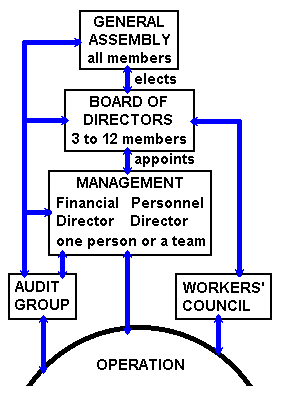
\includegraphics[max width=\textwidth]{p30mond}
\end{center}

\textbf{The General Assembly} meets once or twice a year, involves all members and is concerned with major policy issues, such as membership rules, production targets, budgets and distribution of profits.

Its decisions are binding.

\textbf{The Board of Directors} is elected; members are unpaid and serve for 4 years, meeting once a month. They review and co-ordinate operations, appoint the Management who attend meetings but cannot vote.

It sets Operational policy.

\textbf{The Management} are the executive body of the business, serve for 4 years and have full administrative control.

\textbf{The Audit Group} consists of 3 members elected by the General Assembly who inspect the accounts, sometimes calling in experts. They alert managers of problems (which they are expected to resolve), produce information for the General Assembly, and may alert the Co-op of crisis.

\textbf{The Workers Council} consists of all members. It meets monthly to discuss matters such as wages, conditions and safety. It represents the work force on the Board of Directors.

\textbf{The Operation} covers the basic activities of the system.

\section*{DIAGNOSIS}
At the Metasystemic level, all four VSM functions may be clearly identified.

\textbf{System 5: Policy}

The General Assembly deals with the major policy issues and elects the Board to set Operational policy in its monthly meetings. The Board provides the monitoring function whereby the rest of the Metasystem is seen to operate within policy guidelines.

\textbf{System 4: Long Term Planning}

Long terms plans are drawn up by the Management and sent to the Board for approval. Some debate may follow.

\textbf{System 3: Optimisation}

This is the responsibility of the Management and seems to be taken seriously. They discuss "synergy" between the Operational elements. The Audit group is System 3*, and is a crucial element of System 3 activities. Its job is to provide the information needed to complete System 3's model after the usual information from the business has been obtained. All companies have some sort of audit function - Mondragon seem to have realised the importance of theirs.

\textbf{System 2: Stability}

The Mondragon philosophy provides an extremely effective stabilising system. There are further System 2 bodies like production scheduling and cash flow control. But generally everyone seems to work together well, and conflict of interests get resolved easily.

\textbf{System 1: Operation}

In 1982 the General Assembly decided to change the basic working procedures within the Operation. It was felt that on the shop floor members lacked motivation and that more participation was needed.

They reorganised the production lines into autonomous work groups of about 8 people in which everyone could do all the jobs. Instead of working with a time horizon of 45 seconds , each group had to complete its task in 16 minutes. This gave people time to make a phone call, or have a quick cigarette or whatever.

In the washing machine factory they changed a 300m line with 70 people into 7 lines 30m long, each with 8 people. The change led to a self-organising system, more motivation, and improved productivity and quality.

\textbf{This system of autonomous Operational elements uses performance indicators.} These measure quantity, quality and costs. The daily indicators are measured (e.g. the number produced). Each week they estimate the more subjective measures (e.g. safety, tidiness, autonomy) and give themselves marks out of 10. This number has to be agreed with the foreman who has the final say.

Each work group has responsibility for maintenance, quality, design and so on. At monthly meeting they monitor production targets, discuss problems, arrange training and so on.

\section*{CONCLUSIONS}

\section*{System Design}
Throughout the description of how the Mondragon co-operatives function I found it hard to believe that the system had not been based upon the VSM. In the five years since the Doughnut proposals at Suma I have been attempting to introduce performance indicators, long term planning functions and the like, and almost everything I have been proposing is standard procedure at Mondragon.

Perhaps the only aspect that could be improved is the statistical analysis of the daily information to generate Algedonics automatically. As far as I can tell, they inspect all the information they generate.

\section*{Participation in Policy}
It has always seemed fundamental that all members of a co-operative have the ability to affect policy at all levels and Mondragon seem to adhere to this principle. Within the co-operative all members make policy at yearly meetings, and occasionally at emergency General Assemblies called by a minimum of 10\% of the co-op. During my visit to the Refrigerator factory there were notice boards everywhere full of information on the policy issues which were to be debated at the next General Assembly.

\section*{Representative Management}
They give their elected managers "full administrative authority" although they insist that this can only be maintained if the manager has the trust of the workforce. (He can be removed by an emergency General Assembly.)

It's clear that some Metasystemic functions must be performed without continuous consultation with the work-force (for example long term plans) and at Mondragon they seem to have found a balance between complete authoritarian control and the lack of clear decision making that comes from having to discuss everything with everyone.

The model which was offered to us was that of a busload of people who instruct the driver as to where they want to go, and then leave the details to him. Once he's been instructed, the rest of the people on the bus leave him to operate the brakes, steer and accelerate as he sees fit. The passengers can also direct him to drive more safely, or get another driver if he's no good. But basically it's up to him to drive the bus.

Finally ..

The Mondragon structure seemed to me to be an example of both efficiency and co-operation based firmly upon autonomy and participation. The VSM diagnosis revealed no major flaws, even in the details of how Operational information is gathered.
\chapter{PRELIMINARY DIAGNOSIS}\label{PRELIMINARY DIAGNOSIS}

\section*{IDENTIFICATION OF THE 5 SYSTEMS}
The Viable Systems Model is based on 5 systems which are seen as fundamental to viability.

If all 5 systems are working well within you organisation, then you can say that the basic functions needed for viability are present. If they are not, then your organisation is not viable in the terms defined in this pack, and you will need to change your organisation to ensure viability.

The purpose of the Preliminary Diagnosis is to identify the 5 systems needed to ensure viability, and to draw them on a large VSM diagram which represents the parts of your organisation in its totality.

If any are not present, they will need to be designed and added to your organisational structure.

If any existing parts of your organisation do not fit into one of the 5 Systems, then they are not crucial for viability and may be unnecessary.

\section*{Preliminary Diagnosis - How it Works}
I was told this story by a colleague (referred to as GB) who lectures in Management Studies, and who uses the VSM as a tool in his consultancies. It gives such a clear picture of the use of Preliminary Diagnosis that I decided to include it at this point.

He was telephoned one morning in connection with the proposed amalgamation of several businesses into an alliance designed to enable the member companies to combine their strengths, and thus compete more effectively in exporting their products. The group had done some preparatory work, but needed advice quickly. A meeting was scheduled for 2.00 pm that afternoon.

Usually, a consultant needs several days to assess the situation and gather the background which is essential for sound advice.

This was clearly impossible.

So, GB arrived for the first meeting with a large piece of paper on which was drawn the outline of the VSM, that is the Operational units and Systems 2, 3, 4 and 5.

As the meeting proceeded, he began to ask questions about the proposed organisation and to fill in the boxes in his VSM diagram. Operational units: the member companies. And so on.

After the proposed organisation had been described, some of the boxes were empty and GB began to probe "How do you intend to ensure that the member companies work together in a more effective manner - won't you need someone to examine the various possibilities and to look for synergy?"

Basically, he was looking for something to write in the System 3 box.

This is the essence of the Preliminary Diagnosis. You define a function, look for the bits of your own enterprise which does it, and write it in on the relevant part of the diagram.

The VSM is so thorough in its model of how a business works, that GB's clients were overwhelmed with "his" insight and made aware there were several aspects of the organisation they had completely overlooked.

And all of this without any preparation.

In your case, assuming you are looking at an existing business, the insights are unlikely to be so staggering. Problems with viability will have arisen and been dealt with, and somewhere the functions needed for viability will have been implemented. The question is - are they adequate?

But whatever the context, you will be mapping your own organisation onto a VSM diagram, and this process is bound to affect the way you look at your enterprise.

\section*{Step 1: DEFINE THE SYSTEM TO BE DIAGNOSED}
\textbf{PURPOSE: To clarify the boundaries of the System-in-Focus.}

During the diagnosis which follows, there are times when it's easy to lose track of exactly what is being studied. So its essential to begin the Preliminary Diagnosis with a clear statement of the organisation (or the parts of the organisation) you are looking at. Throughout this guide, this will be referred to as the System-in-Focus.

Before starting the Diagnosis and the identification of the systems needed for viability, you should list all the parts of the System-in-Focus as you see them.

The list should be exhaustive as it will be referred to throughout the Preliminary Diagnosis. It will contain the Operational parts, the accounting functions, the management functions and so on.

In compiling the list, keep one eye on your sketch of the various recursions and ensure that the items on the list refer only to the system-in-focus. It's likely that your first list will need revision and that one or two items will belong to another recursion. Check it carefully.

As the Preliminary Diagnosis proceeds, you will be able to take the items on your list and allocate them to one or other of the 5 systems within the Viable Systems Model. Thus, the list will gradually disappear.

If your organisation is perfectly Viable, the list will disappear completely and there will be 5 well defined systems giving the basis for viability.

If not, either

\begin{itemize}
  \item some new jobs may have to invented
\end{itemize}

or

\begin{itemize}
  \item some existing jobs are not needed for viability and can therefore be considered as redundant.
\end{itemize}

\section*{Step 2: DRAW THE VIABLE SYSTEM MODEL IN OUTLINE}
The diagnosis of your organisation will proceed by drawing a large diagram which will represent your System-in-Focus as a whole system. At this stage, the outlines of the three main parts of the VSM - Operation, Metasystem and Environment - will be sketched in. Between them they represent the overview of your System-in-Focus in its totality.


\section*{DRAWING THE VSM - from Step 2 - drawing the outlines}
\textbf{Notes:}

\begin{enumerate}
  \item There is a tendency to see this diagram as hierarchical. The Boss over the Workers. From my experience, (and from discussions with Beer) this is completely wrong. The Metasystem is there to service the Operational elements. It has a different perspective, or over-view, as it has to consider the collection of Operational units in its entirety, but the need to have power over the people in the Operation is strictly limited to its job of cohesion. It can only wield power if the system is in danger of breaking apart.

  \item Everything which will be drawn on this diagram must refer to the System-in-Focus. At a later stage you may want to delve further into the workings of each Operational element, so you will drop a level of recursion, define a new system-in-focus and start again. For the time being the diagnosis will concentrate upon the System-in-Focus you have defined.

\end{enumerate}

\section*{Step 3: SYSTEM ONE - THE OPERATION}
\textbf{PURPOSE:} To specify those parts of the system-in-focus which undertake System One (primary) activities.

The first system in the Viable Systems Model is the entire Operation which will be composed of several Operational units.

The Operational units undertake the System-in-Focus's basic activities.

They will all be (smaller) Viable Systems in themselves, and thus must be able to maintain a separate existence.

System One generates wealth and in a business, each element can be considered as a profit centre.

If you are a manufacturing business, System One is the production units, the teams of people and machines which actually do the manufacturing.

If you are a programming co-op, System One is the programmers or teams of programmers, perhaps divided into various specialist areas.

If you are looking at a more complex organisation, you may have a System One which includes manufacturing, distribution, and warehousing.

System One sounds straightforward, but is actually one of the most difficult areas to define clearly. For example, in the examples given above the computer department was a System One in the programming firm, but the computer department in the manufacturing company would have a support role and would therefore not be part of System One. Some people who are in basically service areas such as engineering maintenance may consider themselves important enough to be System One.

The question is: are they part of what the organisation is really about, or are they back-up, facilitators, or support? If the answer is the latter, then they do not qualify as System One.

You are now in a position to go back to the original list of jobs carried out by your System-in-Focus, and to list those which between them make up System One.

Note: Each Operational unit is a VSM at the next recursion down and thus will include both the physical aspects and the management of one aspect of the Operation. So, for example, the trucks and drivers and the management of the transport department are found within that Operational Unit.)

\section*{DRAWING THE VSM - from Step 3 - adding the Operational Units}
\begin{center}
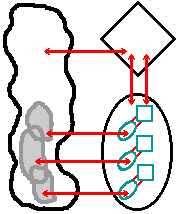
\includegraphics[max width=\textwidth]{3vsm_aou}
\end{center}

This diagram shows the VSM with three Operational units high-lighted.

There is no reason why you should have three, although it is unlikely that you have more than eight.

The diagram also shows the parts of the environment which are specific to the Operational units.


\section*{Steps 1, 2 and 3: Example}
\begin{center}
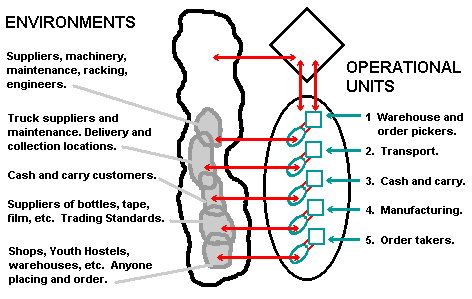
\includegraphics[max width=\textwidth]{3suma}
\end{center}

So far you have drawn the VSM in outline and added

\begin{itemize}
  \item the Operational units

  \item the external environments which are specific to each of the Operational units.

\end{itemize}

At this stage the Suma VSM looked as follows:

SYSTEM IN FOCUS: Suma Natural Food Wholesalers

MISSION: Warehousing and Distributing Natural \& Ecological products.


\section*{Steps 1, 2 and 3: Another Example}
\href{http://www.radicalroutes.org.uk/}{Radical Routes} is a group of co-operatives in the UK who have formed a loose Federation in order to promote their activities.

They found the VSM an interesting environment with which to look at their problems and carried out a Preliminary Diagnosis on their own.

They began with System One and thought \textit{So what are we really about ... what are the primary activities?} Understandably, they began to draw the Operational elements as the activities of the federation; for example fund-raising, education, stimulating interest about co-operatives and so on.

I was then invited to meet with them and discuss the work they had done.

After some discussion we decided that a more useful way of looking at System One was as follows:

\begin{itemize}
  \item Radical Routes exists to service the member co-ops

  \item The primary activities of Radical Routes concern the member co-operatives themselves

  \item Therefore the Operational units are the member co-operatives and all the activities of the federative body are Metasystemic.

\end{itemize}

After this fundamental re-think we spent the rest of the afternoon looking at the design of the whole system in these terms.

A diagnosis based on the original definition of System One would have come up with entirely different results.

So please note:

\begin{enumerate}
  \item The way that you define the Operational elements largely determines the way that the rest of the diagnosis proceeds.

  \item This is crucial to a useful outcome. The Operational parts need to be primarily concerned with their own internal issues (minding their own business) while the Metasystem parts can only function if they have the ability to prioritise the over-view. If these are wrongly chosen, then the system cannot function effectively.

  \item There are no absolute rights and wrongs. A model is only correct to the extent it is useful. Radical Routes may well have reached interesting conclusions from their initial guess, and only the final outcome (did it work?) can judge which diagnosis was the better. Pause for breath .....

\end{enumerate}

At this stage it is sensible to review what's happened so far, and to think about how the Preliminary Diagnosis is going to proceed.

So Far ...

You have drawn in outline three shapes which represent your System-in-Focus in its totality, and its external environment.

You have defined your System-in-Focus and its Mission Statement.

The System-in-Focus has been defined in two parts:

\begin{enumerate}
  \item The Operational units which carry out the primary activities, which DO whatever is needed to fulfil the Mission Statement. and ...

  \item The Metasystem which is there to provide whatever services are needed by the Operational units to ensure they hang together in an integrated form.

\end{enumerate}

You have listed all the parts of your enterprise which are part of the system-in-focus as you see them.

You have extracted the parts which between them make up the Operation or System One.

You have drawn these Operational units on the outlined VSM with their corresponding local environments.

The Next Stage ...

Having listed the Operational units in System One, you will be moving on to look at the Metasystem, and it is important to bear in mind the following thoughts:

\begin{enumerate}
  \item The Metasystem is charged with doing whatever is needed to enable the Operational units to come together to make a single, integrated, coherent system. It may be defined as providing the "glue" to make sure the autonomous departments don't drift apart into a number of isolated bits.

  \item The Metasystem will always be concerned with the Operation as a whole. It may be looking at the interactions between the Operational units or at the implications of a policy decision, but at all times it is involved with System One in its entirety.

  \item It will not be concerned with internal matters within the Operational units. This would be comparable to expecting you to be involved with the mechanics of the beating of your heart. In general the Operational units are seen as autonomous and the Metasystem is concerned only with the way they interact.

\end{enumerate}

\section*{Step 4: SYSTEM TWO - STABILITY AND CONFLICT RESOLUTION}
\textbf{PURPOSE:} To identify those parts of the System-in-Focus which ensure that the Operational units interact in a stable manner.

\subsection*{Why think about stability?}
Without exception, all systems with interactive parts, regardless of their nature, have stability problems.

Anyone who's had the misfortune of trying to ride a bicycle with a buckled wheel down a steep hill will know how an unstable system can behave, and why the consideration of stability criteria is an essential part of any design.

Instabilities between people are just as universal. Look at young children in the playground, or marital break-down, or the way communes inevitably collapse.

Nation States exhibit extreme instabilities, the arms-race being the most concerning outcome.

But whatever the particular case, the need for some way of dealing with instabilities is essential, otherwise the organisation will shake itself to pieces.

The argument goes:

\begin{enumerate}
  \item The parts of a system will invariably have conflicting interests.

  \item These conflicts will tend to lead to instabilities.

  \item Instabilities left unchecked become destructive, and the system will begin to oscillate. (I want it! Give it to me! No I won't!)

  \item To deal with this, any viable system must have a System Two for:

\end{enumerate}

\begin{itemize}
  \item resolving conflicts

  \item dealing with instability

  \item damping oscillations

\end{itemize}

\section*{A System 2 story}
Suma used to have a three floor warehouse in which goods were moved up and down by fork trucks lifting pallets through holes in the floor. Every now and again, a pallet would fail to find a home and the top floor operator would send the pallet back down to the middle floor. The operator on the middle floor would think "this isn't my pallet - it will have to move back up" and the pallet would go up and down, up and down, all day.

The motion of the pallet was exactly like a yo-yo, or in Beer's terms it was oscillating due to conflicting interests between Operational elements.

The resolution of this problem was to get the operators from each floor to meet, to discuss the problem and then to resolve it: "Look someone has to agree to take this pallet and its definitely nothing to do with me - I only do beans and grains." "Yes, but you're the only one with enough spare space ... my floor's too full already" Eventually agreement was reached, the pallet was found a home and the oscillation stopped.

A general strategy for System Two in this context would be a series of rules for allocating pallets. If it were thorough enough, oscillations would be rare.

Beer lists many examples of instabilities in industry which lead to oscillations. One of these came from his observation that the stocks of raw materials in a production shop vary dramatically. Sometimes they run so low that everyone is worried that they will run out, sometimes they are so high that the available space runs out and storage becomes a problem.

The stock levels oscillate between these extremes. Again a System Two needs to be designed to stabilise this situation, for example Just In Time ordering, which keep inter-process stocks to a minimum.

In some cases System Two may be a nuts-and-bolts system like a production schedule or a timetable which will ensure that conflicts do not arise as several parts of an organisation are all clamouring for the same resources.

In other cases, System Two may be more subtle. In Mondragon the predominant System Two was the methods they employed to share resources and support each other's businesses. My attempts to find out how they deal with conflicts between competing businesses were always answered with "but we share all profits anyway ... why should there be a problem?" In the case studies which you read you will notice that System Two in a co-operative is generally covered by the "co-operative ethos." It seems clear that in an organisation in which the common good is paramount, instabilities will be fairly easy to resolve.

If the company ethos is competitive, if your success is measured against the performance of others, then it's much more likely that your interests will be exactly the opposite of others. So the temptation will be to act in such a way that your successes will bring about others' failures. And of course everyone else is doing the same.

Obviously, a co-operative will not be completely free of this kind of thing: there is only so much money to spend and the various Operational elements will compete for it. Some people are naturally competitive. Cash flow will need to be controlled. The financial System Two will have to be designed.

However, in most of my applications, working within a co-operative ethos means that there is already a pervasive System Two, and this gives the System two designer a head start.

\section*{Summary}
System Two is charged with dealing with the instabilities which inevitably arise between the Operational units.

Every organisation must have a System Two:

\begin{itemize}
  \item to resolve conflict

  \item to deal with instabilities

  \item to damp oscillations

\end{itemize}

\section*{DRAWING THE VSM - from Step 4 - adding System Two}
\begin{center}
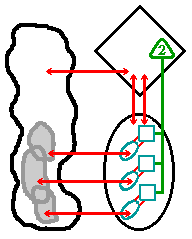
\includegraphics[max width=\textwidth]{3vsm_as2}
\end{center}

The diagram to the right shows the VSM with System 2 added (in green).

Note that System Two is part of the Metasystem (it sits in the diamond) and that it passes through every Operational unit.

Thus, it looks at the entire collection of interacting System One units with a view to resolving conflicts, dealing with problems and creating stability.

System Two has been drawn slightly larger than usual for emphasis.


\section*{Step 4: IDENTIFICATION OF SYSTEM TWO - examples}
You have now drawn in System Two on the VSM diagram.

Examples of System Two are as follows:

\subsection*{System Two: Suma}
System Two is generally performed by the co-operative ethos which prevents major conflicts between members.

The weekly Rota allocates members to various jobs according to departmental needs, and thus stabilises the problem of too many people in one area and not enough in another.

There must be good cash flow control, thus stabilising the tendency for huge surpluses and overdrafts.

The recent stock-control system stabilises stock holdings and avoids an oscillation between vast stocks and goods going out-of-stock.

\subsection*{System Two: Mondragon}
Mondragon provides a System Two by sharing profits and by mutual financial support. This resolves any conflict of one business benefiting at the expense of another.

\subsection*{System Two: School}
The timetable is regularly cited as the ideal System Two.

It takes care of double-booking, and resolves the conflict of several teachers all wanting the same rooms, projectors etc., etc.

\subsection*{System Two: Manufacturing Company.}
System Two is the production schedule which performs the same stabilising function as the school timetable. It resolves the conflict which could emerge in competition for limited resources.

\section*{Step 5: SYSTEM THREE - OPTIMISATION}
\textbf{PURPOSE:} To identify those parts of the System-in-Focus which optimise the interaction of the Operational units, and to update the VSM diagram accordingly.

\section*{A System Three Story}
Consider a Viable System consisting of several dozen people trying to put out a fire by running to a nearby lake, filling a bucket and running back to throw the water on the fire.

Each person with a bucket is an Operational unit. Each will be absorbed with his own job.

The Metasystem - which may be one person sitting on the top of a ladder - will look at the whole system and may say "Keep to the left on the way down" (\textit{System 2} - stopping continuous collisions) or it may think about optimisation.

Eventually she may realise that if everyone forms a chain and moves the buckets from hand to hand, then you only have to move the water and buckets, and not your own body weight. The same job can be done, but only a fraction of the energy needs to be expended.

The extra efficiency which is generated as a consequence of acting as a whole system rather than an un-coordinated collection of parts is called synergy, and the generation of synergy is the essence of System Three.

\section*{The Job of System Three}
In all cases, System Three has the same function:

\begin{itemize}
  \item It is poised with an over-view of the entire collection of Operational elements.

  \item It looks at the way these elements interact.

  \item It considers way of optimising the overall efficiency of the entire collection of Operational elements.

  \item This improvement in efficiency is called synergy, so System Three's job is usually described as generating synergy.

\end{itemize}

Synergy is of course the essence of co-operation: four people working together co-operatively may be twice as efficient as four people doing the same work on their own.

The current task is to describe the ways that System Three functions within a viable system.

\begin{itemize}
  \item How does it deal with the Inside and Now?

  \item What does it do to generate synergy?

\end{itemize}

\section*{System Three - the Diagrams.}
\begin{center}
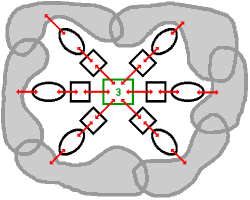
\includegraphics[max width=\textwidth]{s3_ool}
\end{center}

System Three is best thought of in the middle of a whole lot of activity. All around it the Operational elements are concerned with meeting the demands of their own environments (answering the phone, getting the orders completed on time, scheduling the trucks ...) and interacting with each other.

System Three sits right in the middle of all this activity, thinking about ways of optimising the whole thing.

Although this depicts nicely the relationship between Systems Three and One, it's a bit messy, and leave no room to illustrate the interactions between System Three and the rest of the Metasystem.

So \textbf{it's usually drawn above a stack of Operation elements like this}:

\begin{center}
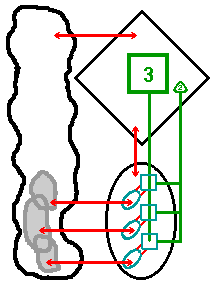
\includegraphics[max width=\textwidth]{3vsm_as3}
\end{center}

This diagram shows the VSM with System 2, reduced to fit into the Metasystem's diamond and outlined, and a large System 3 added for emphasis.

It's shown interacting with three Operational elements, although not as clearly as in the first diagram.

This arrangement has much more in common with the human System Three - the base brain - which sits on top of the spinal column and optimises the working of the muscles and organs.

We can now begin to describe the ways in which System Three over-sees the collection of Operational elements, looking for synergy.

\section*{The Resource Bargain}
System Three usually controls the purse strings. Resources are ultimately limited, and so it's essential for System Three to allocate them according to the global needs of the System-in-Focus.

This requires System Three to look at the whole of System One, and to allocate resources so as to optimise performance.

Thus System Three may say: "Your job is to get the goods to the customers in the most effective way, and we will give you £200,000 a month to do it. And as long as you do the job properly, you will continue to get the money."

Obviously this will require lots of negotiations between all the Operational units and System Three, and it leaves System Three with enormous amounts of flexibility to generate synergy "Hmmmm .... if I put a few more resources into production they say they can be 17\% more efficient. But that will mean cutting back on procurement and cut our margins by 1.52\%. On balance that looks fine ...a much better allocation of resources."

In a team, the resource bargain is more likely to involve allocation of people. "You do this and I'll do that, and things will work better ..." In a jazz band it could be allocation of time "The sax solo went on longer than expected, I'll cut down my break on keyboards."

But whatever the particular example, manipulation of the resource bargain provides a means of optimisation.

\section*{Operational Accountability}
Once an Operational unit has been allocated its share of resources, it must demonstrate that it's using them properly.

Thus the Operational elements must be accountable: they must be able to show that everything is proceeding as agreed with the Metasystem.

This is an essential aspect of the resource bargain; it's the way the Operational element demonstrates that it can justify the continuing allocation of resources from System Three.

The human Viable System has without doubt the most thorough network for demonstrating that all is going well. Every part of the body sends continuous messages to the base brain which knows just what's going on in real time. During periods of intense activity, this information is used by the base brain to modify the flow of adrenaline to the organs and muscles to optimise their operation.

Beer's design for an equivalent system in an enterprise is based upon near real-time monitoring of all System One activity and a set of statistical filters assessing the information. The System Three office would have a big green light or a continuous tone which would mean "everything is OK". As soon as any of the measurements moved outside acceptable limits, the light would go off, and other signals would identify the source of the problem.

But whatever the design, the Operational units must have a way of justifying their allocation of resources.

\section*{The Command Channel (1): Intervention Rules.}
Inevitably there will be problems. What happens if one Operational unit begins to deteriorate due to machinery breakdowns, all the trained personnel leaving suddenly, or something completely unexpected like a flood? In some cases the unit can cope, in others it may not and this may threaten the survival of the entire enterprise.

Clearly, there must be rules in place to deal with this. In certain situations System Three has to be given the mandate to intervene within an Operational element.

For example, if the information shows that productivity is down, wastage is up and morale has collapsed, then it's essential for System Three to intervene. Intervention means loss of autonomy and is only permitted when the cohesion of the whole system is at risk.

Intervention rules must be defined clearly, so that each Operational element knows it will be left alone unless it transgresses the agreed norms.

All of this needs careful design.

Beer has a simple recipe for deciding on the level of autonomy which can be allocated to an Operational element . He says autonomy should only be forfeit when system cohesion is at risk. So, if the actions of one Operational unit threaten to shake apart the whole system, its autonomy must be forfeit. In all other cases it should be left to function within the resource bargain - it is, after all, designed to be autonomous.

\section*{The Command Channel (2): Legal \& Corporate Requirements.}
By now it should be clear that the approach used here is in no way hierarchical and uses authority only as a last resort. The practice of senior management to interfere in all aspects of the business has been dismissed not for political reasons but purely from the \href{https://vsmg.lrc.org.uk/screen.php?page=variety}{Laws of Variety} - it just can't be done competently.

However, here we have a case in which the Operational Units, conceived as working with maximised autonomy, must obey a higher authority.

System Three will ensure they pay taxes and stick to legal guidelines on (for example) Heath and Safety and employment.

System Three will also ensure that the Operational elements stick to company Policy, regardless of the financial advantages. This may concern equal opportunities, or remuneration or a commitment to give money to charity.

Some years ago a Suma member suggested that we set up a separate department staffed mainly by part time labour from the job centre. Figures suggested we could make money this way (labour costs were significantly below usual levels) but the proposal was well outside our Policies on employment and pay. Corporate Suma said no.

\subsection*{System 3* Audits and Surveys.}
The final link between System Three and the Operational Units is called System 3*, and goes directly to the Operational bits of System One.

It's job is to provide whatever information is needed to complete the model which is needed by System Three.

It's inevitable that System Three will encounter situations in which it just doesn't have enough information to know what's going on. Regardless of the kind of information it may need, this is the job of System 3*.

It may involve a study on buildings or machines or on the incidence of back injuries or on any aspect of the goings-on within the Operation.

System 3* is often referred to as looking for signs of stress. In the original physiological model System 3* was based upon a nerve called the vagus which reports back to the base brain on signs of stress in muscles and organs.

In the VSM this function has been extended to give System 3* the job of topping up the information needed by System Three.

\section*{SUMMARY}
System Three deals with the whole of System One (all the Operational units) and looks at the way they interact.

System Three is concerned with improving the overall performance of System One, so its main job is optimisation. In simple terms, System 2 deals with problems between the Operational units (its function is stability) whereas System Three makes positive suggestions as to ways of improving overall performance.

In order to do this, System Three allocates resources of people and money. It may see that by cutting back in one area and by re-allocating those resources in another, the overall performance may improve.

System Three needs to know how each Operational unit is doing, so it can continuously re-think its own plans in the light of changing circumstances. It therefore needs the Operational units to be accountable. Ideally, System Three will have a complete and up to date model of everything it needs to know about System One.

From time to time System Three will need further information about the Operation and will ask to do audits and surveys.

And finally, System Three must have the ability to intervene within an Operational unit if it believes that unit is threatening the viability of the whole system.

\section*{DRAWING THE VSM - adding System Three}
Note: Remember this is the Preliminary Diagnosis which is concerned only with the identification of the five Systems. So the job at this point is only to specify which parts of your enterprise do System Three stuff. The lines which you have drawn are to sketch in the connections between System Three and the Operational units. Later all of these interconnections will be dealt with in more detail, but it's far easier to build up a framework for the entire system-in-focus, before delving into the way the five systems interact.

\section*{System Three: Examples}

\subsection*{Small Group System Three}
All of the Optimisation functions are carried out by the team-mind which constantly assesses what's going on, and acts accordingly. Accountability is total as the people doing the work and the managers are one and the same. A complete analysis of all System three function revealed no inadequacies whatsoever.

\subsection*{Suma 1991}
The Finance Offer and Finance Committee allocate budgets on a yearly basis. This is thrashed out in discussion with the various departments, and decided on the basis of optimisation - how to allocate the money so as to get the most from Suma as a whole.

The personnel budgets are decided in a similar way. Departments are asked how many people they can manage with, and this is optimised.

Accountability is very patchy. There is no standard departmental system to account for how the budgets are spent. Major mistakes are obvious anyway, but regular quantified reporting has yet to be established.

Audits are common and emerge from areas of interest. How much are we spending on back treatment? What skills do we have that are unused? Do we need to rotate jobs more regularly? Reports will be produced and the subject discussed.

Intervention rules have still to be defined. In theory a department could become inefficient (especially in slack times) and no-one would know. Thus an acceptable lower performance level and intervention rules are not possible.

\subsection*{Mondragon Co-ops 1991}
The body which articulates System Three for a group of autonomous member co-operatives describes itself as \textit{stimulating the co-ordinated joint development of the co-operatives incorporated in the group} Synergy is perhaps the single most used word when talking to people about this function.

There are many examples of how this is carried out.

\begin{itemize}
  \item Centralised buying, marketing
  \item Transfer of technology
  \item Inter-trading
  \item Joint R \& D
  \item Optimised product ranges
\end{itemize}

These functions are carried out by meetings of managers from the various member co-ops.

\section*{Step 6: SYSTEM 4}
\textbf{PURPOSE:} To identify those parts of the System-in-Focus which are concerned with Future plans and strategies in the context of environmental information.

An example: a company may have one year of its lease left. A number of possibilities are available: it could re-negotiate, the lease move to another rented site, buy an existing building or build a new one. Each of these options needs to be researched in some depth, and the most likely alternative selected. Throughout this process, System 4 must be referring constantly to System 3, to ensure that the Operational constraints are considered. How many square feet? How much head room? Access to motorways? How much office space? Any specialised manufacturing facilities?

Clearly, when System 4 has recommended a number of options, it will require site visits from System 3, and the interchange of ideas will continue.

\subsection*{PRELIMINARY QUESTION}
WHICH PART OF YOUR SYSTEM-IN-FOCUS PRODUCES STRATEGIES FOR FUTURE PLANNING?

(Remember, this is about the System-in-Focus, not about the embedded S1 Viable Systems ...

You may find that there is no focus for System 4 in your organisation. In the co-operatives I've worked in, this kind of activity is usually undertaken as a last resort.

The Viable Systems Model asserts that for this function to work properly it must have a continuous focus: somewhere in the System-in-Focus someone must be looking at the environment and thinking about ways of dealing with a largely unknown future.

In the following section, you will find an exercise concerning System 4, and a worked example. When you have completed it, you should have a good idea about the System 4 activities which you organisation ought to be undertaking. When its finished, you should think about the question posed on this page: (What is System 4 in your structure?) and decide whether you think it can do the job of continuously adapting to the future.

\section*{System 4 Exercise}
%\begin{enumerate}
%  \item 
\subsection*{List the activities of System 4 under the following headings}

ACTIVITY

RESPONSIBILITY

TIME SCALE

PRIORITY

  \begin{itemize}
    \item Activity: What sort of planning?

    \item Responsibility: Who has to do it?

    \item Time Scale: C for current. One year if it needs to be dealt with in a year.

    \item Priority: A, B, C, D or E (A the most urgent - They could all be E)

  \end{itemize} 
\subsection*{Revise the list}
The list contains all the activities which you System-in-Focus is undertaking in order to guarantee adaptation to the future. Is it complete???

The list refers to the System-in-Focus. Go thorough it and identify the items which refer to the embedded System One Operational elements. (Example: For Suma relocating refers to the System-in-Focus. Replacing a Fork Truck refers to the Warehouse which is System One) Cross out everything which belongs in System One. They will be dealt with at the next level.

%  \item 
\subsection*{Group the activities into coherent groups.}
Several of the items on the list may be concerned with (say) Product Design, or Technological Development, or Market Potential.

%  \item 
\subsection*{Draw a diagram showing the overlaps.}
The diagram below is the one I did for HWMC in 1986. At the time we were in the process of relocating and the other major areas were rationalising the machinery (selling some, buying others) packing for new customers, and our relationship with our single major customer.

The areas of overlap indicate how the various issues relate to each other, and the bit in the middle which has three areas overlapping (the move, new machinery, relationship with major customer) is the centre of real concern about the future.

Each shaded area indicates where collaboration may be needed.

You will probably need to re-draw this diagram several times.

If the diagram you drew has no areas of overlap, then something should be done. It means that the members of your organisation concerned with future planning are working in isolation, and this is obviously not a good idea.

However it is not uncommon for Research and Development to become obsessed with technological issues and to ignore Market Research. And for Corporate Planning to degenerate into purely economic terms which pay little heed to R \&amo; D and Market Research.

%\end{enumerate}

\section*{Worked Example: HWMC 1985}
There were several more entries but they seemed to fall into four categories. After a few attempts the diagram looked like this.

\begin{center}
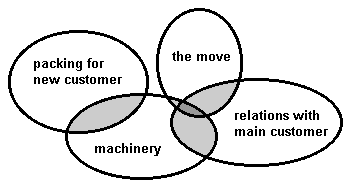
\includegraphics[max width=\textwidth]{3stp7we}
\end{center}

This illustrated the main activities and how they overlapped, and thus gave a good representation of the issues with which System 4 had to deal.

\section*{DRAWING THE VSM - From Step 6 - adding System 4}

\subsection*{Step 6: IDENTIFICATION OF SYSTEM 4 - examples}
You have now drawn in System 4 on your VSM diagram.

Examples of System 4 are as follows:

\subsection*{System 4 - Suma 1991}
Future planning is given occasional consideration by groups and individuals. The Futures committee looked at possibilities for diversystem-in-focusication but didn't produce any proposals. A recent five year plan decided only to continue to proceed in same mode. In summary, there is no continuous focus for System 4 activity, and thus very little future planning.

\subsection*{System 4 - Mondragon}
Mondragon has a firm commitment to Research and Development; its System 4 keeps in touch with developments in all aspects of robotics, production techniques, new products, and computerisation.

Mondragon has built its own R \& D facility.

It is in touch with those aspects of its external environment which may exhibit novelty (e.g. European Space Project).

It is currently looking seriously towards the unified European market in 1993 and planning accordingly.

\section*{Step 7: SYSTEM 5}
PURPOSE: To identify those parts of the System-in-Focus which are concerned with Policy.

Policy concerns the ground rules which affect everyone in an organisation.

In the Viable System, policy is the domain of System 5. It may best be described as "Top Level Ethos", and its role is to become involved in the complex interactions between Systems 3 and 4.

System 5 has two main functions:

Firstly, to supply "logical closure": The loop between systems 3 and 4 is potentially unstable and must be overseen Metasystemically.

Secondly, to monitor the goings on in the whole organisation. These must be constrained by policy.

There is, of course, nothing to stop System 5 wielding its own authority (for example ... demanding that System 4 begins to study a particular issue and that System 3 responds to this ... and that the eventual outcome is passed to the Operational units to be elaborated into a production plan) but this is a rare occurrence.

System 5 provides the context, the ground rules, the ethos.

Who is System 5???

If your mind works like most of us the answer to this question will be something like Henry Ford or Walt Disney or some other hero who dominates the policy of the enterprise. (Any colour as long as it's black ...). Beer has written at length about the way that all elements of the Viable System are mutually dependant, and that giving one any more importance than another is clearly wrong. (How viable would Aristotle have been if any of his major organs had closed down??) The question of who System 5 actually is has to be answered very simply as everyone involved in the system. At the governmental level it should be described as "the Will of the People", within the co-operative it's the same and systems must be designed to ensure that's how it works. (Again notice that Mondragon seem to have grasped the essence .. they describe their General Assembly as "The Will of the Members").

At Suma, the Hub/Sector system evolved to provide a means of ensuring that policy can involve all members on a continuous basis. To my knowledge this is the only System 5 which works in this way with large numbers: usually systems will involve a few meeting a year.

\section*{DRAWING THE VSM - from Step 7 - adding System 5}

\section*{Step 7: SYSTEM 5 - examples}
\textbf{You have now drawn in System 5 on your VSM diagram}

\textbf{Examples of System 5 are as follows:}


\section*{REVIEW: THE VSM IN ITS ENTIRETY}

\section*{Step 8: PRELIMINARY DIAGNOSIS}
By now you have:

\begin{itemize}
  \item Listed the Operational elements.

  \item Identified System 2.

  \item Listed the five functions of System 3 and identified it.

  \item Listed System 4 activities and considered who does them.

  \item Considered policy and the extent to which it represents the views of the members.

\end{itemize}

You have also put all of this together on a large VSM diagram, which will give a picture of your System-in-Focus in its totality.

Now cross out those parts of your organisation which appear on the VSM from your original list.

Remember to be clear about the System-in-Focus. Anything about the internal workings of the Operational elements should not appear on this diagram. (So .. in Suma's case .. the optimisation techniques used within each department don't appear. They are the concern of the next (smaller) level of organisation. The boxes 2, 3, 4 and 5 refer to the whole of Suma.)

If you can't put anything in some of the boxes, you are in the same position that I was. There was effectively no System 4, except when it was unavoidable, at Suma.

At this point you should take some time to consider the implications of the preliminary diagnosis.

Some of the five functions will be performed by people or departments which clearly don't have the resources to do the job adequately.

In some cases the entire Metasystem will be performed informally, and that may be fine (See Case Study on HWMC).

There will be some jobs which are left on your list after filling in the VSM. Are they necessary? Some will be support jobs, like machine maintenance. The computer department is a facilitator, which makes things happen more smoothly and quickly. Both these jobs are clearly useful.

But what about some of the committees? Are they really essential to viability?

**At the end of this process you should have

\begin{itemize}
  \item Identified the major parts of your System-in-Focus which render it viable.

  \item Considered the parts which seem to be inadequate.

  \item Identified any parts which don't map onto the VSM and therefore don't have anything to do with viability.

\end{itemize}

This concludes the Preliminary Diagnosis.

**
\chapter*{JANUS INTERLUDE}\label{JANUS INTERLUDE}
\addcontentsline{toc}{chapter}  {JANUS INTERLUDE}
\markboth{JANUS INTERLUDE}{}

\begin{center}
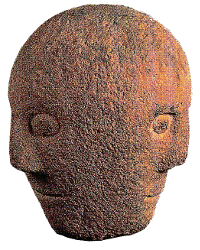
\includegraphics[max width=\textwidth]{janus_rock_200x250}
\end{center}

Janus has rightly been adopted as the god of whole systems. He can look forwards and backwards simultaneously, and thus symbolises the closed loop at the heart of all cybernetic systems.

This Janus interlude is included at roughly the halfway point in the book to provide the reader with a perspective on where he's been and where he's going.

Looking back ...

Having completed the Preliminary Diagnosis, you should by now have a thorough feel for the form of the model.

\begin{itemize}
  \item The separation of Operation, Metasystem and Environment

  \item The small VSMs nested recursively within the Operation

  \item The four Metasystemic functions

\end{itemize}

If you have been drawing the pictures, you should by now have a number of large VSM sketches, showing the five systems and the bits of your organisation which do those jobs, and you will probably have had a Eureka! or two, as the VSM version of organisational reality unfolded.

Looking forward ...

So where do we go from here?

I admit that my first few attempts at using the VSM finished here, despite a few nagging doubts about Beer's Laws and Axioms, which didn't really seem to fit in anywhere.

After much further reading and discussion it became clear that the job had only been half-completed. YES, I had identified the five systems at various levels of recursion, but NO, the diagnosis was by no means complete.

Consider now, the Viable Vehicle Model, or VVM, a guaranteed fool-proof methodology for the diagnosis and design of any vehicle, regardless of size or the terrain on which it must travel, based cybernetically on the invariances in vehicular functioning.

The VVM is composed of 5 systems:

\begin{enumerate}
  \item Some means of propulsion
  \item Some means of steering
  \item Something to carry the load
  \item A method of reducing friction
  \item Some way of stopping
\end{enumerate}

Imagine you have completed the Preliminary Diagnosis of your Vehicle-in-Focus (or VIF) that you have successfully identified the five systems, and drawn a big diagram to illustrate their basic relationships.

So what now? Is the VVM diagnosis complete? Again you may have a few nagging doubts about the VIF as a whole. For example, you may be concerned that your design of your Propulsion System One (in this case a very substantial rubber band) is not quite up to the job of moving the Vehicle with the 400 tonne loads you envisage. Similarly System 5 (a large rock on the end of a rope) has been clearly identified as a fine example of the stopping function, but as the vehicle is intended to transport steel in Alaska (and thus has System 4 consisting of skis) doesn't look too reliable.

The overriding questions begin to emerge: Do the parts add up to a workable whole? Are the parts balanced to complement one another?

VVM practitioners will know that the workings of the whole is a very different thing from the workings of the parts. In some cases overall improvements in efficiency may be the result of actually decreasing the capabilities of one sub-unit.

So, if the vehicle is on wheels, are the brakes and engine designed to match the weight and speeds for which the vehicle is designed? If the vehicle is a hovercraft, the engine could be smaller as friction is minimal, but this may present more problems for the design of the stopping and steering systems.

\begin{center}
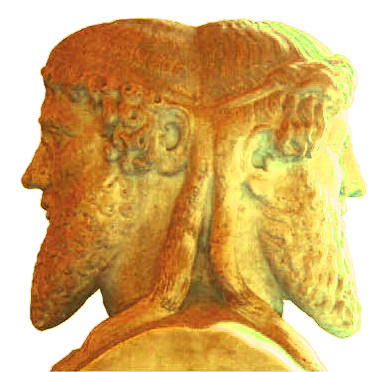
\includegraphics[max width=\textwidth]{Janus_383x372}
\end{center}

The conclusion is:

\begin{itemize}
  \item The design of the whole system must be considered.

  \item Just because the parts are there, there is no reason why they should work together to produce an effective whole.

\end{itemize}

And exactly the same is true of the VSM.

In my initial studies, I had not looked at the way the parts interact, how they work together to generate a well-designed whole, how the capabilities of the regulatory systems balance the problems they are dealing with.

Everything which follows is about balance.

The essence is well-balanced, whole-system design.

This is where the forward-looking head of Janus is looking.
\chapter{DESIGNING AUTONOMY}\label{DESIGNING AUTONOMY}
In this Section you will begin to look at the way that the various parts of your organisation work together.

At the end of the Preliminary Diagnosis, you will have a picture of the way your enterprise looks in terms of the "building blocks" which compose it.

The rest of the manual looks at the interaction of these building blocks, and is concerned with ensuring that the whole thing works together in an integrated form.

The essence is organisational balance: of ensuring that the bits which are charged with overseeing the Operational units have the capacity to do their job properly.

The first element of generating this balance is to give each Operational unit as much autonomy as the organisation can handle, without degenerating into separate and isolated parts.

\section*{Autonomy or Authority}
If you have organisational problems such as lack of efficiency or jobs just not getting done there are basically two options:

\begin{itemize}
  \item You can appoint managers who have the authority to make sure that these problems get dealt with.

  \item You can design a system which ensures that the problems are dealt with autonomously.

\end{itemize}

The first option has been used for hundreds of years in all kinds of society and it is only recently that its limitations are becoming clear. The Management Gurus in the United States are now coming out with statements like "Train the hell out of your workers and then get out of their way".

This new emphasis on making all workers more autonomous has been obvious to people in co-operatives for decades - what has been lacking is the systems needed to ensure it works properly. There is no point in saying "OK ... you're all autonomous now" and expecting the rest to take care of itself.

The first essential is for each Operational unit to be clear about its role within the whole organisation and should therefore produce its own Mission Statement.

This may take some negotiation with everyone else, but will ensure that the Operational unit works as an integrated part of a greater whole.


\section*{Allocation of Resources}
Whatever your organisation, the Operational units will need resources. They will need money and people in order to carry out their function.

This is the point at which the design process can begin.

System 3, which oversees the collection of Operational units must have a financial aspect which is concerned with the overall financial picture for the business. It is the job of financial System 3 to allocate resources.

Usually this will occur in the yearly budget rounds. Each unit will say "We need $x$ pound; $x$ pound; $x$ pound; in order to do our job", System 3 will add it all up and say "Sorry, we don't have enough to give everyone everything they want, who can make cuts?"

This process will continue until either the necessary cuts are made .. or .. System 3 will make decisions about who gets what, in the light of what's best for the whole organisation. (That is ... it optimises the allocation of resources).

In most cases, the allocation will only happen once a year and thereafter, each Operational unit will do its job according to the pressures put upon it by the market or other parts of its own organisation.

This one way process (here's the money you need, and that's the end of my job ...) works reasonably well as long as everything proceeds as normal, but is totally incapable of dealing with problems.

The usual situation is as follows:

\begin{itemize}
  \item Each Department gets its budget.

  \item Each Department carries on with very few guidelines except to maintain things as normal.

In the event of a dramatic collapse in productivity within a department, it is possible that no-one would know for months and severe damage could be done to the organisation.

The solution is clear - each department must be accountable.

This is the alternative: System 3 says: "Here are your resources - you can have them as long as you do your job in the way we agreed."

\end{itemize}

Thus:

\begin{itemize}
  \item Each Department has a clear Mission Statement and performance targets.

  \item Each Department gets its budget so it can carry out its mission.

  \item Each Department must account for its performance on a continuous basis to justify its use of resources.

  \item System 3 monitors performance to ensure resources are being consumed in the optimum way decided in the yearly budget rounds.

\end{itemize}

\section*{Dealing with Problems: Intervention Rules}
The question must arise: "If each Operational element is given autonomy, how do you stop standards from sliding?"

The question is valid. A protocol must be in place which can deal with the possibility of a group of people loosing heart and of letting their performance deteriorate.

The first part of the solution is accountability: if performance is measured and the figures are monitored, then at least the deterioration can be noticed.

The second part is to define clear performance standards which the people working within that unit can aim for.

The final part is to agree the terms on which any severe problems can be dealt with. This may be something like:

If productivity falls to 85\% of the usual level and doesn't improve for 10 days, then autonomy is forfeit, a trouble-shooter will be appointed to assess the situation and recommendations will be made to the rest of the co-operative.

The details of this statement will vary depending upon the situation, but the loss of autonomy must be an essential element.

The nature of the intervention rules should:

\begin{itemize}
  \item be agreed in advance by both the Operational unit and System 3

  \item give the unit a fair amount of time to deal with the problem itself, thus giving autonomy a chance to work. Immediate intervention would undermine autonomy

  \item be designed to ensure that the survival of the whole enterprise is not at risk. Thus, only fairly severe declines in standards should warrant loss of autonomy.

\end{itemize}

The essence of this system is to both encourage and underwrite Operational autonomy while ensuring that the worst case scenario is dealt with quickly and fairly.

To do this, a continuous interaction between the Operational unit and System 3 is essential.

The unit should be free to pursue its own development and respond to the demands of its environment, but within the constraints of being part of a larger whole.

\section*{Step 9: Designing Operational Autonomy}

\subsection*{Example 1: Mondragon}
.

Mondragon exhibits most of the necessary elements of this system of autonomy.

\begin{itemize}
  \item Autonomy is recognised as an essential element of an efficient organisation.

  \item Accountability is discharged using daily and weekly performance indicators.

  \item The people working within each unit have to keep weekly work levels up to a particular standard, so they are free to come in late after a carnival as long as they make it up later.

  \item There is continuous monitoring (through the Audit Groups) and if any business in a Sector exhibits problems a rescue squad is sent in.

\end{itemize}

\subsection*{Example 2: Council Workers}
While I was writing this pack, the council arrived to re-lay the drive around my house. Two men arrived and put wooden boards into the ground to determine the level and orientation of the drive. Some time later, another crew arrived to lay the tarmac. They brought the tarmac around using a big tractor which didn't fit between the boards and smashed several of them into splinters.

I asked what they intended to do and they said "We were told to use this tractor and lay the tarmac so that's what we have to do" So they laid the tarmac without guides.

Diagnosis:

\begin{itemize}
  \item No Operational autonomy. The workmen didn't have the freedom to modify their plan after the situation changed. They had to do "What they'd been told to do".

  \item No monitoring. The man who could alter the plan was miles away and had no idea what was happening.

\end{itemize}

Clearly the situation is unworkable, unless the original plan is so thorough that it takes care of every eventuality, or unless the Man In Charge is there for the entire duration of the job.

Inevitably, the plan cannot cope with the complexities of the situation and the Supervisor has several jobs which he is supposed to supervise going on simultaneously.

The solution is (of course) to give the men doing the job the autonomy to control it themselves, but that is completely alien to the culture.

I discussed this with one of the workmen who agreed. "But we're all supposed to be totally stupid and only able to do what we're told."
\chapter{BALANCING THE INTERNAL ENVIRONMENT}
  \label{BALANCING THE INTERNAL ENVIRONMENT}
In this Section you will be looking at the internal environment of your organisation - the entire complex of interacting Operational units and Systems 2 and 3 which are there to stabilise and optimise.

If it is out of balance, then there will be instabilities (lots of conflict, people competing for the same resources, confusions about who should be doing what), a lack of optimisation (clear ways that overall efficiency could be improved, but no way of either planning it or of getting it implemented), and the Operational units may be working in isolation from the rest of the organisation.

The solution to these kinds of problem is to ensure that there is a balance between the complexity of the problems affecting the Operational units, and the capabilities of Systems 2 and 3 who have to deal with them.

The approach is as follows:


\section*{Internal Environment: Systems 1, 2 and 3}
The Inside and Now is the internal environment of the organisation. It includes the Operational elements, and Systems 2 and 3 which have the job of optimisation, stabilisation, gathering the information needed for these functions, and passing information to and from the rest of the organisation.

In the next few pages we will be looking at the design of all of this.

But first: review all the elements of the Inside and Now by considering your VSM diagram of Systems 1, 2 and 3. It will look something like this.

\textbf{The Question now is:
How can we ensure that all of these aspects of the Inside and Now are properly designed?}

\subsection*{Operational and Environmental Interactions}
If you take your VSM picture and look at the Operational units and their environments, you will have something like this.

In a study on a federations of co-operatives, these two perspectives proved to be of crucial importance.

\subsection*{Environmental Overlaps}
The environments consisted mainly of markets and suppliers and the crucial overlap was the delivery areas. Many of the problems in establishing the federation could be dealt with by re-defining the delivery areas to concentrate on local service. Suppliers (the other main part of the environments) also required consideration. By making each warehouse specialise in a limited range of suppliers, the expertise of the group could be improved.

\subsection*{Operational Connections}
The movement of goods between warehouses proved to generate interesting ideas. One warehouse with a surplus could use the others to reduce it. Short best-before-dates could be moved more quickly. Shortages in any part of the federation could be dealt with quickly by supplies from another.

**

Having made the Operational units as autonomous as possible the next step is to look at these two channels and to see if any issues can be dealt with in this way.

The steps involved in this procedure are given below.

**

\subsection*{Step 10 Operational and Environmental Interactions}

\section*{Designing Systems 2 and 3}
In the previous pages we have looked at

\begin{itemize}
  \item Making the Operational units autonomous.

  \item Operational accountability and allocation of resources.

  \item Intervention rules.

  \item Environmental intersects and how to use them to make System 1 more efficient.

  \item Operational interactions and how they may be used to to make System 1 more efficient.

\end{itemize}

**

All of these techniques enable the Operational units to deal with day by day problems without interference. They are ways of generating the maximum amount of autonomy within the limits of the larger whole.

The question now is:
"Do Systems 2 and 3 have the capabilities to deal with their jobs of stabilising and optimising the internal environment???"

**

You have already identified the parts of your organisation which do these jobs at the moment.

\begin{itemize}
  \item You will have a rota or some sort of scheduling system to make sure people know where they should be working.

  \item Someone will have to decide yearly budgets.

  \item At some stage there will be discussions on optimisation - "If we put more emphasis on manufacturing and less on publicity we could do lots better ..."

\end{itemize}

\textbf{But are your existing systems adequate?}

As the rate of change of markets continues to escalate it becomes more and more essential to monitor and deal with problems on a continuous basis - and so monthly committees are becoming progressively more useless.

How thorough is the information you have from your Operational units? How good is the model of System 1? How up-to-date? If this is inadequate, then any decisions made by Systems 2 and 3 will be made in some degree of ignorance.

After thinking about issues like this you may decide to increase the capabilities of Systems 2 and 3 in order to ensure they can do their job. This may involve more time, more people, more thorough monitoring or whatever.

Whatever you decide, it is essential not to interfere with the autonomy of the Operational units, unless it is absolutely necessary.

The steps involved in completing the internal balance are given on the next page.

\section*{Step 11: Completing the Internal Balance (Summary and Conclusion)}

\section*{Designing the Internal Balance: Examples}

\subsection*{Example 1: Suma}
Suma's internal balance was restored as follows

\begin{itemize}
  \item the departments were made autonomous.

  \item a Finance Officer and Personnel Officer were appointed.

  \item information systems were created to measure daily performance statistics in the sales office and manufacturing departments.

  \item weekly business information was produced and given to all members.

\end{itemize}

The combination of local autonomy, improved information systems, and the new System 2 and 3 jobs restored the balance.

\subsection*{Example 2: National Manufacturing Company}
A major national company was the subject of a VSM diagnosis which revealed severe shortcomings in the way that information on stock levels was sent from the local warehouses to the central manufacturing facility.

This led to incorrect assumptions as to the products which needed to be produced and huge inefficiencies at the factories. On several occasions late information would result in a change of plan, involving resetting a production facility which had taken eight hours to set up.

A study of the internal environment revealed that establishing accurate information systems was all that was needed to restore the internal balance.

\subsection*{Example 3: (Hypothetical) Federation of three Warehouses}
The traditional approach to ensure that the three warehouses work together efficiently would be hierarchical: appoint 3 managers and put them all under the control of a general manager. In VSM terms, this is the use of the command channel (C4) but this inevitably interferes with the autonomy of the warehouses and thus their ability to deal with their own environments. Consider the other alternatives:

\begin{itemize}
  \item Design the delivery areas so the warehouses don't compete.

  \item Agree to audits and surveys.

  \item Study the interchange of goods between warehouses.

  \item Agree performance targets and report back.

  \item Design stabilising systems to schedule deliveries.

\end{itemize}

Once these systems have been established, the need for any sort of authoritarian system should become completely unnecessary, and Systems 2 and 3 may be designed with relative ease.

\subsection*{Example 4: Chile 1972}
Beer's work in Chile was essentially to integrate the entire social economy into a single system using the VSM.

He established communications links between most of the nations factories and a central gathering point in Santiago which implemented Systems 2 and 3.

Each factory measured its performance daily and sent a set of indicators through communications systems based on microwaves and telexes and in some cases messages on horse back.

A suite of computer programs analysed the indicators, and sent any alerting messages straight back to the relevant factory. (This was 1972 and computers were still very expensive. Most of this would be done by Micros today, thus enhancing local autonomy).

The integration of most of the nation's industry into a single system had some dramatic consequences.

During 1972 the CIA initiated a strike of 70\% of Chile's transportation. They had embarked upon a policy of "destabilisation" and had bribed the owners of the trucks to refuse to work.

Immediately, the alerting signals began to flood into Santiago. No raw materials here, no food there.

This began a period of intense activity as the signals were processed and plans were produced to provide as much of the nations transportation needs with the 30\% which was under the control of the Government.

Because the information systems were so thorough, the people in Santiago knew exactly what was needed, by whom, what trucks were available and so on.

During the next 36 hours all the emergencies were dealt with, everything which was needed was delivered and some factories said that they had never had better service.

For this situation, Systems 2 and 3 were clearly able to deal with the demands of the Operational units, despite the fact that 70\% of the distribution system was unavailable to them.

Most of the success is due to the conception of an integrated economy, and to the information systems which enabled the people dealing with the crisis to know just what was involved: their models were thorough and current.

The US Congress reports of that era show a great deal of surprise at the stability of Chile under Allende, and that in order to attain their goal of bringing Pinochet to power they had to make far greater efforts than they had expected.
\chapter{INFORMATION SYSTEMS}
  \label{INFORMATION SYSTEMS}
%this section whole section is boxed int
In this Section, the importance of information systems will be discussed, and techniques will be developed to ensure that a thorough system is developed to make sure the various parts of your organisation have the information they need to operate properly.

It cannot be stressed too strongly that a good information system is an alternative to authoritarian management - it can render unnecessary organisational techniques based upon authority and obedience.

If the appropriate information is measured and feed-back is used to modify the way people work, then many organisational issues take care of themselves.

This Section covers real time information systems based on performance indicators, self-assesment using these indicators, and the generation of the alerting signals called algedonics.

\section*{Information Systems: The VSM approach}
If you look at the Inside and Now of your VSM diagram there are several areas in which information is crucial to good design:

\begin{itemize}
  \item The Operational units must be accountable - they must find measures of what they do and make sure the appropriate information gets to System 3.

  \item System 3* does audits and surveys - it is an information service to System 3, looking at whatever is of relevance.

  \item System 3 must have a thorough model of all that it needs to know about the goings-on within the entire complex of interacting Operational units. Otherwise it will be making decisions in ignorance.

  \item An information system must be capable of generating alerting signals so that the organisation can find out that something has gone badly wrong as soon as it happens. These signals are referred to as "algedonics".

  \item System 4 is charged with adapting to environmental change. It will need information about the external environment so it can produce strategies. It will also need a good model of the internal capabilities so it knows what tools it has at its disposal.

\end{itemize}

All of these factors require thorough information systems.

Traditionally information systems within a business are primarily concerned with financial information. They generally involve historical figures, so that after the monthly figures are produced someone may say "We have just realised that the business lost money last month because of something that happened in Factory 27" Which is, of course, too late.

The other aspect of traditional information systems which is superseded in VSM theory is the production of huge print outs from a data base, most of which are never used.

Central to the VSM approach is the production of only what is important. If information says "All seems to be going as usual" then nothing needs be done. Consequently, there is no point in printing the report.

The information systems used in the VSM are fundamentally different from traditional systems in that:

\begin{itemize}
  \item they are based upon performance indicators which measure whatever is important within each Operational unit, and not just financial information.

  \item they are based upon daily measurement so that problems can be identified the same day.

\end{itemize}

\section*{Closing the Loop}
The overall principle is clear - closed loops work and open loops don't.

In traditional businesses the loop is closed in a number of ways: Work hard - get paid - keep the job - satisfy the boss - work harder and so on. The loops are closed with reward systems involving money (and sometimes job satisfaction) and with punishment systems involving the fear of reprimand and eventually losing the job.

All of this works as long as the monitoring systems are adequate enough to keep an eye on the work force most of this time. The problem is the schism that emerges between the motivation of the manager (as much work for as little money as possible thus maximising profits) and the work-force (the opposite).

\section*{Example 1: Suma}
The following example is taken from some of the experimental work at Suma:

\begin{enumerate}
  \item \textbf{The Operational Unit.} This is the pre-packing department which is given a budget and autonomy and expected to do its job properly. It must therefore be accountable to the rest of Suma. That is - it must be able to demonstrate that everything is proceeding in a satisfactory manner.

  \item \textbf{Performance Indicators.} It was agreed with the rest of Suma that the factors which must be measured are:

  \begin{itemize}
    \item Productivity (number of bags per person per day)

    \item Wastage (as a percentage of bulk weight)

    \item Number of Out of Stocks (number of stock lines not available due to packing problems) Stock Holding (value of goods bagged down)

    \item Morale (subjective happiness rating of people doing the packing - the difference between morning rating and evening.)

  \end{itemize}Between them, these indicators provide a complete picture of everything which goes on within the department. Any one of these indicators can identify a problem - for example productivity may be fine, wastage might be improving, the stock holding may be wonderful, but the out-of-stocks may be disastrous. Examination may show that the department is concentrating on efficient long runs, but ignoring the requirement to keep most of the pre-pack lines in stock.

Conversely, out-of-stocks may be fine, but this might be at the expense of productivity. (Lots of inefficient short runs ... )

You can only discharge accountability by monitoring all the indicators.

  \item \textbf{Algedonics.} The key to all of this is to ignore everything which says "All is well".

\end{enumerate}

So you examine the time series and say nothing if its going up and down as you'd expect it to. But, if there's a sudden leap or plummet, something important has happened, and it's crucial that the alerting signal which is called an algedonic is generated. Beer describes algedonics as signals which scream "Ouch it hurts!"

\section*{Cyberfilter}
Cyberfilter is a computer program which takes care of all of this stuff on indicators and algedonics.

You work out your performance indicators at the end of each day and put them into the program. The history of each indicator can be displayed as a graph. It then analyses the graph and tells you if something significant has happened, that is, it generates algedonics.

The program also does several other things involved with short term forecasting and planning, but its main functions from my point of view are:

\begin{itemize}
  \item a simple means of recording performance indicators and

  \item the generation of algedonics.

\end{itemize}

Consider the following crises:

\subsection*{a) The scales break}
Suppose that the scales (which are used to weigh all the pre-packs) get damaged slightly and thus all the packs are 10\% overweight. No-one notices during the day, although there is slight discomfort about the lower yields.

At the end of production, the indicators are worked out and it's clear that wastage has leaped from 2 to 10 \%. In this crisis, everything is checked, the problem is identified and an engineer is called.

(This actually happened a few years ago, but wastage was only monitored infrequently, and no-one really knows how long we were giving away vast amounts of food ... )

\subsection*{b) Change in Personnel}
After some years of efficient production the members of the department feel like a change, and new personnel are chosen. Some training takes place, but after the new personnel are established all the indicators start to slip.

Initially the information goes back only to the pre-packing department, but after a further two weeks no improvement has been made, and the algedonic is sent to the co-operative as a whole and an enquiry is made.

The previous workers are called back in, the situation is sorted out with more training and perhaps some re-allocation of people, and the original performance levels are regenerated. (Again this happens all the time in co-operatives but as there are no performance indicators, the new team has very little basis on which to learn. In some extreme cases, the decline in standards resulted in a department being shut down, but only after the quarterly accounts showed that money had been lost.)

\section*{Summary}
The essence of all this is the design of an information system which:

\begin{itemize}
  \item Underwrites departmental autonomy.

  \item Provides the feed-back to enable a department to learn and adapt.

  \item Ensures that Operational autonomy can only continue as long as they are working to standards set by the needs of the whole organisation.

  \item Only responds with useful information (no more monster computer print-outs to feed the shredder).

  \item Responds to information which is only a few hours out of date.

\end{itemize}

\section*{Example 2: Mondragon}
One of my original problems with the idea of performance indicators was how to deal with performance which is not easy to measure - you can record the number of boxes produced, but how do you measure something like tidiness or morale?

One solution to these problems came from the Fagor refrigerator factory in Mondragon.

They had changed their production line into a series of autonomous work groups in order to address problems of motivation, and had identified performance indicators as the appropriate means of handling information.

As expected, they measured productivity and other quantifiable aspects of their working situation, and this gave them a new degree of autonomy.

For example, during my visit to Mondragon there were a series of festivals which lasted all night and (as expected) the production figures fell dramatically on the following day. This is not seen as a problem as long as the figures rise on subsequent days and the weekly average reaches the usual standard.

All of this is under the control of the people on the shop floor - the algedonic is only generated if the weekly average is affected.

Thus a comprehensive monitoring system can enhance departmental autonomy.

But they were also able to deal with less tangible elements.

They do this by negotiation: Once a week a representative of the work group meets with the foreman and they go through a number of performance indicators. As an example they discuss autonomy which is registered on a scale of 0 to 10. The group is aiming at complete autonomy and may feel it had almost got there: "We think 9 for autonomy". The foreman may disagree "But on Wednesday you couldn't deal with a problem and had to ask me to sort it out for you. I think 6." Eventually they may agree on 8.

All these numbers are written up and displayed on notice boards. They don't plot graphs, but the flow of numbers provides a reasonable picture of the way things are going, and provides the feed back which is one of the more important aspects of this system.

This concept of negotiated performance indicators opens up many possibilities. In a co-operative it seems more likely that the negotiator would be someone who used to work in a particular department, understands how it functions, and has an interest in maintaining its standards.

\section*{How to Design the System}

\section*{1. Performance Indicators}
Negotiations are needed between the department in question and whoever is responsible for the allocation of resources. (Remember this is also designing the accountability systems which complete the resource-bargain loop between Systems 1 and 3).

The question is "What numbers do I regularly quote when I'm talking about how well the day has gone?" For example "Only three tonnes of muesli all afternoon." or "What a good day! I completed four pages of the ledger."

These indicators need to satisfy both the department and the resource allocator that they give a complete picture.

It will then be the responsibility of the department to measure and plot them every day.

\section*{2. Algedonics}
Some variation will be inevitable. It may take some time to establish what an algedonic actually is. So ... 5\% variation in productivity is fine as long as the variations even out. A continuous decline for 4 days is unacceptable and constitutes an algedonic. A 10\% variation needs to be examined. And so on.

If you decide to use Cyberfilter, this kind of decision will still have to be made. The responsiveness of the program has to be established, or it may churn out algedonics every time someone sneezes.

\section*{3. Time Periods.}
Each indicator must be studied individually. You must then decide how long it should take to deal with problems, and how long a problem can be permitted to continue until the viability of the whole co-operative is at risk.

So ... you have 5 days to deal with wastage problems, 10 days to get out-of-stocks back to acceptable levels, and so on.

These time periods must be agreed in advance, as when a crises hits the system, the framework for dealing with it must be already established.

\section*{4. Loss of Autonomy}
Assuming an indicator becomes unacceptable and continues at that level beyond the pre-agreed time, then the whole co-operative gets notified and that department loses its autonomy.

The nature of this loss should again be designed. It may involve a complete analysis of the problem, or the appointment of an agreed trouble-shooter or whatever.

But again this should be agreed in advance.

\section*{Step 12 Examine your Information Systems}
% Box with 3 items numbered 12.1 12.2 12.3
 Consider your current information systems. How do you measure what is happening within each department? How do you ensure that each department is doing the things it is supposed to do? Do you need systems which alert you when something goes wrong, or would it be immediately obvious anyway? How up-to-date is your financial information? If you started to loose money today, how long would it take for you systems to realise?
 
 In the light of the answers to these questions, you should be able to address the crucial issue: How complete and up-to-date is the model of the operation?

If you have qualms about the kind of information systems you currently use, it may be sensible to define and measure performance indicators daily and see how your organisation changes.
\chapter{BALANCE WITH THE EXTERNAL ENVIRONMENT}
  \label{BALANCE WITH THE EXTERNAL ENVIRONMENT}
In this Section you will be looking at the way that your enterprise deals with changes in the environment in which it exists.

There is no point in having a superbly organised internal environment if the enterprise as a whole is completely out of touch with the environment in which it operates. The rate of change of technological advance continues to accelerate, and businesses cannot afford to stand still and ignore the changes in the market. Currently, computer software designers consider themselves lucky if a particular program leads the market for more than a year.

The focus for these issues is System 4 which is responsible for future planning in the context of environmental information which it gathers.

System 4 must provide the balance between the internal Operational units and the outside world, and must ensure that the organisation can adapt to change.

\section*{Graphical Overview}
The following diagram illustrates the relevant parts of the VSM involved in this Section.

The issues which will be addressed in this Section are:

\begin{itemize}
  \item How does System 4 keep in touch with the outside world?

  \item What capabilities does System 4 need in order to formulate its plans which are needed to ensure that the enterprise can adapt to the changes in the environment.

  \item What is the role of System 3?

  \item What is the role of System 5?

\end{itemize}

\section*{Connection to the External Environment}
System 4 is charged with dealing with future planning in the context of the external environment. Clearly, the first job for System 4 is to decide which part of the (infinite) external environment is of direct relevance.

The VSM distinguishes between two kinds of external environment:

The first is the Predictable which can be monitored. Trends may be identified and decisions made accordingly.

The obvious example of this is the way that a market is changing.

In most businesses it is clear that as market trends alter, the business must adapt. Most large corporations spend enormous amounts of money on Market Research and on running experiments in selected areas to assess the mood of the consumer.

The second is the Novel. Things may be proceeding just as you expect and then someone invents the light bulb. Clearly every Viable System must have some provision for coping with the novel, even if it's only being aware of development programs in the relevant areas.

\section*{Connection to the Internal Environment}
System 4 has to be an integrated part of the Viable System. Its main internal connection is through System 3 which is charged with stabilising and optimising the internal environment.

The intense interaction between Systems 3 and 4 was mentioned in the Preliminary Diagnosis. This is essential as all plans must evolve in the context of both external threats and opportunities, and of the internal capabilities of the System-in-Focus.

The example of a new warehouse was given earlier - System 4 needs to look outwards (at possible sites, financing options, etc. etc.) and to look inwards (necessary square footage, headroom, hygiene standards, etc.) and to make a decision in the light of both sets of information.

In practical terms this means that the need for good communications between Systems 3 and 4 must be recognised.

There is no point in having these two essential aspects of viability working in isolation.

\begin{itemize}
  \item The people making future plans must be in touch with, and take account of, the internal capabilities of the organisation

  \item The people charged with the overview of the internal environment must be aware of the plans being formulated by the future planners.

\end{itemize}

\section*{The Role of System 5}
It's clear that at some stage, decisions will have to be made about the investment to be made in System 3 and System 4.

If the balance is not made correctly disaster may ensue:

Too much emphasis on System 3. Internally, the systems may work wonderfully, but without System 4 the products may become irrelevant, e.g. perfectly designed and manufactured Sedan Chairs.

Too much emphasis on System 4. The future planning may be impeccable but the Inside and Now may be incapable of producing the goods. In this case, the kind of product may be exactly what the market needs but their quality or price may make them unsaleable.

An example of this kind of imbalance is illustrated by Clive Sinclair's production of electronic calculators. His research and development was superb, but the organisation was not viable as his production cost were too high. Too much System 4: not enough emphasis of System 3.

It should be noted that his next venture got the balance right. The ZX computers were well conceived and well produced.

It should also be noted that his Electric Cars displayed his first error in System 4: they were not what the market wanted and despite good quality and prices were (in the UK at least) a complete flop.

The decisions about the investment in Systems 3 and 4 have to be made at the policy level. The decision will have to be made in terms of the nature of the business, and the speed with which the market changes.

This is a job for System 5.

\section*{Monitoring}

\section*{Step 13 Design the Balance with the External Environment}

\section*{Example 1: Small Co-operative}
In a small co-operative most of this is taken care of through the mechanics of thorough discussion.

Systems 3 and 4 are the same people and so the necessary communication is straightforward.

The System 4 plans will be made with thorough knowledge of the capabilities of the Operational units.

Allocation of resources must be performed by deciding to put time aside to look at markets, and to formulate plans.

But, basically the system can work well, as long as the need for these functions is recognised.

\section*{Example 2: Large Co-operative}
The perceived need for a System 4 in large co-operatives seems to vary enormously.

Some co-operatives seem to function without any continuous focus for future planning and with sporadic bursts of activity when the need becomes obvious. Most of these co-operatives function in markets which are not in a rapid state of flux, and have survived without a well defined System 4. Their viability depends upon the markets continuing in this mode, or upon the realisation that continuous future planning is a necessary function.

Other co-operatives recognise the need for System 4, which is often carried out by one of the founder members.

\section*{Example 3: Mondragon}
At every level, the Mondragon co-operatives take System 4 functions very seriously.

They monitor market trends, and technological advances and ensure their production techniques are state-of-the-art. They do their own research and development and from the evidence I had from my visit, they are fully adapted to the external environment.

Currently one of their main preoccupations is with the unified European market, and how it will affect their market position.

It is difficult to assess their allocation of resources without a thorough study, but their seem to put equal emphasis on their future plans and simulations and upon the need for efficient production techniques.

\chapter{DESIGNING POLICY SYSTEMS}
  \label{DESIGNING POLICY SYSTEMS}
From the co-operative point of view, the way that policy is made and implemented is without doubt the most important issue. The business must pay its bills and make a profit, but all of the financial issues are constraints: what the co-operative is really all about is defined partly by its mission statement, and partly by the working environment it creates for its members.

Central to this issue is the involvement that everyone has in making policy.

In a small group this is easy: you have a meeting, discuss an issue until some sort of consensus emerges, and the policy is made.

In a larger group the dynamics of large meetings make this difficult, and choices have to be made about the methods of involving everyone in all the important policy decisions, and how to prevent the business degenerating into endless non-productive meetings.

\section*{System 5: The Design of Policy Systems}
Perhaps the biggest problem at Suma in 1986 was that everyone wanted to be involved in every decision and the resulting proliferation of meetings was getting unworkable. While policy clearly requires an input from every member, it had become necessary to get some decisions made only by the members directly involved.

The VSM contribution to this problem was:

\begin{itemize}
  \item to make departmental decisions within each department.

  \item to appoint officers with an overview to make decisions about the interaction of departments.

  \item to make all of this accountable to all members with clear mechanismsto empower any 5 members to call a General Meeting.

  \item to look at all of this and the policy issues on a weekly basis so that there is no chance of policy slipping away from the control of the membership between infrequent meetings.

\end{itemize}

The situation is, of course, not completely clear. The exact nature of "policy" is indefinable, and it is debatable whether some matters should be decided by an officer or discussed by everyone.

The crucial factors are that:

\begin{itemize}
  \item All officers are accountable.

  \item Mechanisms exist to enable members to change the way that officers are operating.

  \item Clear policy issues cannot be made without the majority of all members agreeing.

\end{itemize}

\section*{Step 14: Design of Policy Structures}

\section*{Example 1}
Suma has been discussed at length. If it may be criticised on its policy systems it must be from the point of view of not letting the officers make decisions on their own. Any slight modification of policy - which could be seen as interpretation of existing policy - has to be discussed by the entire membership.

There is little doubt that the weekly Hub/Sector system keeps everyone involved in all policy matters.

\section*{Example 2}
Other large co-operatives handle decision making in different ways.

They may use a weekly meeting of delegates to take the overview of the current situation, and make decisions on their own initiatives (at Suma, delegates report only their Sectors' views). They then have monthly staff meetings to look at the weekly decisions and to make policy. All weekly decisions and agendas may be pinned on a notice board and members may intervene if they feel it is necessary.

Generally this system seems to work, although there are some grumbles about lack of consultation.

\chapter{THE WHOLE SYSTEM}
  \label{THE WHOLE SYSTEM}
In this Section, all the aspects of the Viable System are brought together and looked at as a whole system.

All the individual aspects have been covered in the previous sections on Internal Balance, External Balance, Information Systems, Autonomy and Policy.

The current task is to see how they can all work together as a single, integrated, harmonious organisation.

\section*{Whole System Responses.}
This description is to give you some idea about the way that all of the various systems interact.

I am taking a hypothetical situation at a hypothetically designed Suma in which all my ideas of Viable System design have been implemented. (!) That is ...

The situation: Due to immanent changes in legislation, wholefood shops will no longer be capable of bagging down their own goods. The situation has been monitored for some months by System 4, who has been liaising with the Packing Department and with the Personnel Officer. System 4 has done some market research and predicted that when the new laws come into effect the entire balance of sales is likely to change from bulk goods to pre-packs.

On consultation with System 3, it turns out that there is plenty of spare capacity in terms of machinery but that the number of trained operatives is dangerously low.

Immediately, System 3 organises a training program to ensure that there will be enough trained members should the demand for pre-packs go through the roof. System 4 has also predicted that the new situation may require a further 11 staff. The question is: how sure can we be that the predicted demand for pre-packs will happen? Each department is told to review its personnel and decide if it can cope in the short term if some of its members have to be diverted to the pre-packing department. Meanwhile 4 new members are recruited (as a safety net) and trained just before the new laws come into effect. When the laws change, demand for pre-packs does escalate, staff is diverted according to an optimisation plan worked out in advance by System 3, and casual labour is called in by each department to fill the gaps. Personnel System 3 begins to recruit and train more full time members, and the indicators monitor the Operation looking for signs of stress.

An Algedonic is generated from the order-pickers showing that productivity and accuracy have dropped dramatically. Examination shows that the best pickers have been moved to pre-packing and more training and some further relocation is needed.

Meanwhile System 4 is thinking about diversifying into Fish. System 3 says absolutely no way until there are enough people to cope with the pre-pack surge. And besides, the Hub reports that the membership have serious doubts about the policy constraints ...

\section*{Whole System Design}
The story on the previous page contains a large set of assumptions all of which are necessary for the system to function in the way described:

Systems 3 and 4 must have been properly designed so that they have the capabilities to

\begin{itemize}
  \item monitor the external environment,

  \item access a complete model of the internal environment,

  \item plan in advance,

  \item respond to problems in real time,

  \item continuously re-adjust the plans as the requirements of the external environment changes.

\end{itemize}

In reality, if the demand for pre-packs did suddenly escalate, Suma would be taken by surprise and would move into crisis mode. Lots of untrained casuals would be called in, productivity would fall accordingly, and the implications would ripple through the organisation. Not enough trained people in the warehouse, not enough order pickers, book-keeping affected as admin staff are relocated ...

And so on.

Perhaps the most dramatic difference is that current accountability systems work on a three month period and so major problems (for example a dramatic drop in productivity) would not be noticed for weeks or even months.

\[June 1992 - interestingly enough, in the last few months the possibility of a surge in pre-packs was recognised and a pre-pack co-ordinator was given a budget of 25 days to research the external environments and make proposals (classic system 4 activity) The results were to invest in different machinery which would be capable of responding to any sudden surge in pre-pack sales.\]

The design of all these elements has already been covered in the preceding Sections of the Pack.

It may be summarised in three parts:

\begin{enumerate}
  \item The internal environment must be in balance. Systems 2 and 3 are there to stabilise and optimise the Operational units and thus the entire internal environment - Systems 1, 2 and 3 - must be designed to ensure it works properly.

  \item The balance between System 3 and System 4 must be found. If they are in balance, your organisation will be able to deal both with its internal environment and plan and adapt to the future. If they are out of balance one of these may be done well but the other may be done badly, and thus viability is threatened.

  \item System 5 - the policy function - must be designed to round off the whole organisation. There must be mechanisms in place to ensure everyone is working within the same ground rules. Without a well designed System 5, it is impossible to ensure that all the parts of the organisation are working to the same basic philosophy.

\end{enumerate}

How it all Works ...

As all five systems are continuously interacting, it is impossible to begin at the beginning, because wherever you start, there will have been something else already going on.

But nevertheless, let us begin with the day to day interactions between the Operation and its environment.

In a period of relative calm, each Operational unit will get its orders, do its job, and work according to the criteria set by the whole organisation.

System 2 and 3 will be monitoring all of this and may be looking at some sort of optimisation plan, but generally will not be having much impact on the Operation.

This is like the body at rest. The heart and liver are doing their jobs, in the context of the base brain, but the higher brain functions may be watching television.

Then the situation changes, and System 4 identifies a possible opportunity, (such as the new market need for pre-packs), and begins to assess possibilities.

This is the situation in which the whole system must function in an integrated fashion.

Consider the way your body functions in this situation:

Suppose that the phone rings (while you are asleep) and a friend says "We are going to London, in 15 minutes. If you can get to the station, there's a spare ticket for you!"

Immediately, System 4 goes into overdrive. "15 minutes to get to the station ... no money for a taxi ... got to find my coat and scarf ... its about a 10 minute run ... should be alright."

The System 4 plan is sent to System 3. "Need to run to the station" The plan is sent to System 1 - the Operational units - muscles are activated, the heart and lungs increase their activity drastically.

All of this is monitored by Systems 2 and 3 who supervise the interaction of muscles and organs and the flow of adrenaline.

System 3* monitors all of this looking for signs of strain.. It may well be that the System 4 plan - to run to the station - is outside the capabilities of System 1, and the information systems from System 1 send an algedonic to the brain saying "ouch ... terrible pains in my legs" whereupon the brain will assess the situation and may alter its plan accordingly.

Assuming you are fit enough to carry out the plan, your internal environment will be kept stable and you will get to the station.

Plan complete!

All of this will be within the context of your personal policy systems (for example a plan to steal a car was excluded), and the essence is the continuous interaction of the External and Internal eyes, formulating and modifying plans in the context of policy.

\textbf{Diagrammatic Representation.}

**

Consider the following VSM diagram

The essence of the whole system is the balance between the internal (1, 2 \& 3) and the external (3, 4, \& 5).

Systems 1, 2 and 3 are the Inside and Now, and keep the internal environment stable and optimised and generally working well according to the dictates of their environments.

Systems 3, 4 and 5 are looking at future plans in the light of both the external environment, and of the capabilities of the Operation.

Whole system balance requires that these two aspects, which will often be in conflict, are balanced.

For example, the Sales Director may be willing to place strains on the Operation in order to achieve a profitable sale.

From the point of view of the internal environment, the task is to optimise the use of resources. This may not be in line with what the Sales director wants.

In co-operatives there may be a disagreement between the members who think in System 4 mode (let's go for this opportunity ...) and those who are more concerned with leaving things as they are and maximising the use of internal resources.

Whatever the details, it is crucial to balance the requirements of the external environment with the internal capabilities of the Operation.

This is essence of Whole System Design.

**


\chapter{APPLICATION TO FEDERATIONS}
  \label{APPLICATION TO FEDERATIONS}
In this Section the VSM will be applied to the question of how Social Economy enterprises may join together to form a mutually beneficial federation.

The Section begins with a number of case studies involving attempts by co-operatives in the UK to federate, and contrasts these with the example of the \href{https://www.mondragon-corporation.com/en/}{Mondragon} co-operatives in northern Spain.

Some conclusions are drawn in terms of the Viable Systems Model.

The question of design is then considered by using the preliminary work of Stafford Beer on a federation of Nation States in South America.

The Section concludes with some design consideration which will supplement the step by step methodology developed in this pack, for the specific case of federations of Social Economy enterprises.

\section*{The Federation of Northern Wholefood Collectives}
The FNWC began in the mid 1970's as a result of Reg Tayler's agreement with the wholefood shops in the north of England to buy their goods through him and thus to establish a co-operative warehouse (Suma).

Once Suma was in business the number of wholefood shops in the region began to grow and over a two year period around 60 retail co-operatives were set up, all buying from Suma.

The FNWC was the umbrella for all of these co-ops, and monthly meeting were held to discuss the kind of goods and services which Suma should offer, to welcome the new shops which had been set up and to attempt to direct the future course of the Federation.

The rapid growth and success of the Federation led to a mood of optimism, and it was not uncommon for people to express the feeling that co-operatives had finally managed to make a real impact on society. At that time co-operatives were handling around 60\% of the wholefood business in the UK (according to The Grocer trade magazine).

The Federation began to put a levy on all its sales and managed to collect several thousand pounds over a period of a few months.

The possibility of a number of regional warehouses was raised, as the number and geographical spread of the shops was growing. Clearly a local warehouse would provide the best service, but the economies of scale militated in favour of a large central warehouse, and Suma had just moved to a large new premises and needed the support of all the shops in the federation.

It was around this time that the FNWC began to decline. This was partly because Suma had become well established and thus one of the aims of the Federation had been achieved, but also because there seemed to be a lack of direction as to where to go next.

The money which had been raised all went to pay the debts of a restaurant in York, and thus the opportunity to invest in strengthening the FNWC was lost.

Over the next few years attendance at the meetings began to dwindle and it became grudgingly accepted that the loan fund was not operating successfully. After a couple of recipients got into financial trouble and were unable to complete the repayments, the loan fund was abandoned.

Currently, there is little left of the Federation. Suma has withdrawn its discount to co-operatives, and generally trade is the main area of contact.

In retrospect the collapse of the Federation was due to:

\begin{itemize}
  \item Suma's growth and prosperity thus making some aspects of the Federation unnecessary.

  \item Lack of vision.

  \item Lack of the necessary skills to make it work.

\end{itemize}

\section*{The Federation of Wholefood Warehouses in the UK}
In the mid 1980s, there was a series of meetings to establish a Federation of the 6 wholefood warehouses which were in business in the UK. The supposed advantages were:

\begin{itemize}
  \item The capacity to offer a local delivery service to any shop in the UK.

  \item A coherent marketing policy.

  \item Joint buying thus giving better prices and saving the labour involved in having 6 businesses all buying the same commodities.

  \item The ability to produce and market a series of own label products.

  \item Sharing expertise.

\end{itemize}

Despite the apparent good sense of all this, Suma decided not to join. On the information which was available to the co-operative it looked as if Suma would pay most of the cost of running the Federation and get very little back in return, The problem was that Suma's turnover was as much as the other wholesalers put together, and thus the buying price advantages had already been achieved. There was also a problem with delivery areas. Suma was in competition with some of the other warehouses in certain areas, and this was never resolved. In one particular area, Suma was geographically close but one of the other warehouses had a long term personal relationship with a local distributor.

Consequently the Federation was formed without Suma, and thus was only able to offer its services to half the country. The ideal of a national federation of warehouse was rendered null and void.

Soon after it was established, one of the founder co-operatives went out of business, further weakening the federation. Own-label products were produced, but some of these were in direct competition with Suma's products. Centralised buying and marketing never really happened as the member co-operatives were loath to give up any autonomy.

Currently, two of the warehouses in Bristol are in the process of merging as they were operating within 12 miles of each other. And in Scotland two new warehouses have opened in order to provide a more local delivery service over a large and scattered market.

Generally all of these developments happen in a piecemeal fashion, and there is little sense of planning the distribution of wholefoods throughout the UK in a coherent manner.

There are still problems with the "right" to distribution areas. Suma has recently extended its weekly deliveries into South Wales which is close to the Bristol warehouses. And one of the Scottish warehouses is actively selling in Northern Ireland which has traditionally been part of Suma's area.

Without doubt the attempt to get the co-operative wholefood warehouses in the UK to federate and act a cohesive system has failed.

\section*{Federations of Mondragon Co-operatives}

\subsection*{Introduction}
Mondragon is a small town in the Basque region of Spain which has been the location for an extra-ordinary experiment. During the last 50 years the region has been completely changed by the development of 173 separate co-operatives which now employ over 22,000 people.

Everything about Mondragon is impressive: they turn over about three billion dollars; they re-invest vast sums of money in order to keep their buildings and machinery in excellent condition; they have their own research and development labs which are developing state-of-the-art computer and robotic systems They have their own schools, bank and social security system; and they are completely dedicated to the ideal of co-operation.

There is little doubt that the success of the Mondragon co-operatives is to some degree the result of their ability to form alliances and work together at both the geographical and trade-sector level.

The present diagnosis is concerned with the application of the VSM to the way in which they organise separate co-operatives into a coherent system at the Sector Level.

\subsection*{Autonomy and Cohesion}
Everyone I spoke to was adamant that the member co-operatives - which constitute the System 1 or Operation - are completely autonomous. There were accounts of how the members of a small co-operative which makes heaters refused to bow to a sector decision and merge with a larger co-op. The Metasystem was informed of this decision and its only recourse was persuasion. The relevant personnel returned to the small co-op, presented the arguments for the merger and eventually got agreement. However, the small co-operative could have refused.

In VSM terms, the complete autonomy given to each co-operative may be a little excessive: a mechanism should exist which required the merger in the interest of system synergy. However, as everyone I spoke to at Mondragon seems more concerned with the good of the whole than an individual co-op, the system currently seems to work. It was also mentioned that the small co-operative faced exclusion from the group if it failed to respond to the arguments for merger.

So while there seen to be no formal systems to ensure autonomy has to become subject to system cohesion, the social pressures are enormous.

.

\subsection*{Sectoral Organisation}

\subsection*{System 1: Operation}
The 173 co-operatives in Mondragon are currently re-organising from a regional collaboration to a Sectoral base. They are quite clear that in order to compete in a unified Europe, they need to concentrate on the synergy (their words ...) between enterprises in the same Sector.

For this study, the System-in-Focus will be a collaboration of typically 8 co-operatives in a single sector. Mondragon has several sectors dealing with domestic appliances, castings, food, service industries and so on. The principles on which the collaborations work are identical, although some of the details are different.

In general, it will be adequate to talk non-specifically about viability within a Sector, although specific examples will be given.

Within each co-operative, there seems no doubt that the organisational systems cover all of the aspects of VSM diagnosis that I have been involved with. The system of autonomous work groups and daily measurement of performance indicators (although not the concept of statistical filtration and thus automatically generated algedonics) has been up and running for a decade, and they find it leads to greater motivation, a more enjoyable work environment, greater productivity and higher standards.

\subsubsection*{SUMMARY: SYSTEM 1}
System 1 consists of about 8 autonomous co-operatives.

Each co-operative functions within the same Sector.

Each co-operative exhibits the essential property of being a Viable System embedded in the whole.

The Mondragon co-operative culture is focused on the whole group of co-ops, rather than the single enterprise. This provides the basis for federation.

\subsection*{System 2: Stability}
Perhaps the most astonishing aspect of Mondragon is the systems it employs to ensure all the co-operatives avoid instabilities. The word solidarity comes up time after time, and it's difficult not to be impressed by the feeling that all 22,000 Mondragon worker-members are working together. The concept of one co-operative benefiting at the expense of another seems difficult for them to grasp, and usually my questions about conflict of interests were met with surprise.

However, the Eroski Food Group are building HyperMarkets which are taking trade from the smaller shops in the group. This seemed a potentially unstable situation (different co-operatives fighting for the same market) and looked problematical to me. However, at Mondragon, they don't see a problem for the following reasons:

\begin{enumerate}
  \item If one co-operative in a sector loses money, it is supported by the others. Historically most co-operatives have needed support at one time or another from the group, and this is seen as a system of mutual support. It means that there is absolutely no problem with one shop gaining at the expense of another as long as the combined profits of the group are growing. This seems to generate the view that it's the Sector that matters, rather than the individual co-op.

  \item All wages are the same throughout the Sector.

  \item All profit sharing is made on a Sectoral basis.

\end{enumerate}

Thus, if a small shop is loosing trade due a new hypermarket, it is quite possible that the worker-members in the small shop will see the profits of their own co-operative fall but get higher remuneration at the end of the year as the profits of the Sector will rise.

(Compare this situation with the UK wholefood warehouses. As each co-operative had its own wages system and there was no suggestion of mutual financial support, the interactions were unstable: there was conflict of interests due to competition for a limited market. The lack of any sort of System 2 to deal with this meant that the federation was doomed.)

The Mondragon co-ops, who share wage scales and profits throughout the Sector, have managed to dissolve all these problems. They see this as solidarity: in Viable System Model terms, it is an extremely effective System 2 which ensures the member co-operatives can look beyond the survival of their individual co-operatives and concentrate on the development of the Sector.

System 2 is a prerequisite for the articulation of an integrated Viable System.

\subsection*{System 3: Synergy \& Optimisation}
Each co-operative in the Sector sends its General Manager to a Sectoral General Management meeting. Sector General Management is described as stimulating the "co-ordinated, harmonious joint development of the co-operatives incorporated in the Group" Clearly this is a System 3 function.

Some examples of how they do this follow:

\begin{enumerate}
  \item Joint education, research and development. This includes education at all levels throughout the co-operatives. (Beyond the means of one, possible for the Sector).

  \item Optimised product ranges, trade marks etc.

  \item Being able to offer a customer a complete service. (For example there are several co-operatives which make castings: each now specialises in one aspect, the Sector can offer the complete range. This also required new co-operatives to be established so that the Sector could offer a complete service.)

  \item Centralised buying, publicity and marketing.

  \item Transfer of technology and expertise between co-ops.

  \item Inter-co-operative trading: All the manufacturing co-operatives use Mondragon machine tools and control gear.

\end{enumerate}

Generally it's accepted that there are enormous advantages to collaboration. At the level of the entire Mondragon organisation there are bodies called "superstructural". These include a research and development institute, a Social Security system, a Bank, a Technical College, and a training centre for co-operative and management skills. None of the services which these offer would have been possible without collaboration, and it is certain that Mondragon would not have developed so successfully if the member co-operatives had grown as isolated businesses.

The systems they employ to encourage Sector synergy involve meetings of the general managers of the various co-operatives in a Sector and the appointment of a Sector Manager. It should be noted that the power of decision is delegated up through the usual Mondragon system of General assembly, and that the member co-operatives have to agree to the recommendations.

\textbf{Clearly they take advantage of every opportunity to deal with Sector synergy. System 3 is alive and working well.}

\subsection*{System 4: Future Planning}
The existence of the Sector Management bodies enables the Managers to examine the environment in which they exist and to plan accordingly. This System 4 function is performed with characteristic Mondragon excellence.

The FAGOR group, which manufactures a complete range of consumer products, industrial components, and engineering equipment employs 8,000 worker-members with sales of around one billion US dollars. They produce 30\% of the Spanish home appliance market. The 1989 annual report lists some of the System 4 planning activities which were realised.

\begin{enumerate}
  \item Purchase of a company manufacturing refrigerators and electrical boilers.

  \item Purchase of a company manufacturing car components.

  \item Establishing links with specific European and North American companies for joint R\&D projects in domestic appliances and automation.

  \item Launch of a manufacturing plant in Mexico.

Financing advanced production technologies, leading to highly flexible manufacturing processes.

  \item Allocation of \$21.2 million for R\&D activity.

  \item Collaboration with European universities and research centres in ventures like the European Space Project.

\end{enumerate}

The report also outlines their basic commitment to System 4 Activity. For example: "The new economic situation requires a high degree of innovation."

Clearly they are performing the System 4 activities admirably: they are in touch with their environment and are planning at the Sector level to adapt to future threats and opportunities.

The Mondragon philosophy requires an unprecedented commitment from its members, and part of this is realised by the continuous re-investment of its profits both in R\&D and in improvements to plant and buildings. It also results in continuous training and re-training.

In terms of the mechanisms required to accept the plans, Mondragon continues its emphasis on democracy. The plans are made by the Managers, but have to be passed by the Board of Directors. The system, they feel, is slower than in a traditional company but has the advantage that everyone agrees once a decision is made.

However, despite their perceived tardiness, the results of System 4 activity cannot be seen as inadequate in any sense.

\subsection*{System 5: Policy}
Policy is determined by a General Assembly and is described as "The Will of the Members."

Throughout Mondragon, attempts are made to involve the maximum number of members at the policy level. Currently the entire group is debating the wage differentials and the decision will be made at a meeting of over 1,000 people.

At the Sector level, the General Assembly is composed of the members who are on the Board of Directors of every co-operative in the Sector together with the Audit groups and the Managers. Their tasks are described as "to approve the Groups general policy, approve the budget, and to modify organisational rules"

The Eroski group consists of both the 1928 worker members who run the shops and warehouses and the 152,000 consumer members. In this case the General Assembly is composed of 250 delegates from worker-members and 250 delegates from the consumers. In order to ensure everyone is informed of the issues, there are five preliminary meeting before the General Assembly.

The large number of notice boards throughout the factories that I visited, together with the interest that was shown in issues at all levels (currently wage differentials and restructuring to emphasise the Sectoral rather than the Regional groupings) indicated that everyone has an interest in policy at all levels and the means to express themselves.

\subsection*{SUMMARY - SYSTEM 5}
At the Sectoral Level policy is described as "The Will of the Members".

Everyone in Mondragon seems to be interested in policy decisions and there are mechanisms to express this.

Some reservations must be made on the year gap between meetings. From my experiences at Suma it seems clear that lots of policy issues are happening on a weekly time scale, and that to restrict the members by making a contribution once a year has to be seen as a limitation on their involvement in policy matters.

\section*{Conclusions: The VSM and Federations in the UK and N. Spain}
The first point to make is that the Mondragon co-operatives developed in an entirely different setting to their UK counterparts, and there is a common viewpoint that these differences make any comparison invalid. However, as the VSM provides a different language to discuss these issues, and is concerned with structure rather than with cultural background, these objections do not apply.

As a general point it should be noted that the Mondragon co-operatives were directed by Arizmendi, and his overview (or metasystemic view) was without doubt one of the main driving forces behind the growth of the co-operatives. For example, the establishment of the bank would never have happened as the co-operatives which existed at that time were preoccupied with their own growth, and had to be persuaded that diversion of resources to a bank was a good idea.

Without Arizmendi's vision, its likely that the co-operatives would have developed in isolation.

It's also worth noting that Mondragon offered far more than employment. In post war Spain there was no social security, no health care and no pensions. The vision Arizmendi had of Mondragon was a complete way of life and thus he could ask much more of the people.

In the UK co-operatives exist in a culture where there are other jobs, and a well established system of social security.

\subsection*{System 1: The Member Co-operatives}
In all cases the Operational units of the federation are viable autonomous businesses and from this point of view there is no difference between the Spanish and UK co-operatives.

The basic requirement is that they are prepared to give up some of their autonomy in the interests of coming together as a coherent larger whole, and here the differences begin.

In Mondragon it is obvious that commercial success has resulted from the synergy which comes from various co-operatives working together In the UK the track record is very different: federations have achieved virtually nothing, and co-operatives currently work in isolation with only loose trading links and occasional conferences.

Thus the willingness to divert funds and time into a federation, and to accept limits on autonomy in the interests of the greater whole is vastly different in the two countries.

This may be the fundamental difference, and the basis behind the differences in the Metasystem which are discussed in the following pages.

\subsection*{Allocation of Resources}
The Mondragon co-operatives allocate enormous amounts of time and effort to their Metasystemic activities. Each Sector has its managers and assemblies, and there is continuous investment in services which can be offered to the whole group. These include:

\begin{itemize}
  \item Banking

  \item Research and development

  \item Financial advice

  \item Business rescue teams

  \item Preferential loans

  \item Technical advice

  \item Training institutes

\end{itemize}

In the UK co-operatives seem to be loath to allocate any resources whatsoever into activities of this kind. The umbrella organisation for worker co-operatives (ICOM) has had to find ways of financing itself as the membership fees were insufficient, and in general co-operatives can find very little reason to consider working together, and consequently are unwilling to divert resources into Metasystemic federal activity.

In the UK none of the services listed above have been funded by member co-ops. If they exist at all they have been set up independently, and then offered to co-operatives for a fee.

The conclusion is clear: the Mondragon co-operatives have allocated vast amounts of time and money into the creation of a Metasystem charged with "co-ordinated harmonious joint development". In the UK there is no such investment and consequently no Metasystem and no federal activity.

\subsection*{System 2 - Stability}
Mondragon stability systems may be listed as follows:

\begin{enumerate}
  \item Mutual financial support for all member co-operatives: This ensures that loss of sales in one area as a consequence of new sales in another is not a problem.

  \item Wages and profit sharing on a Sector Basis.

  \item Guaranteed relocation of staff throughout the Group.

\end{enumerate}

These factors are all entirely absent from the UK co-operative movement, and thus many co-operatives find themselves in a competitive situation. Generally it has been impossible to resolve conflict of interests and the over-riding factor has been the self-interest of the individual co-operatives.

System 2 is a prerequisite of any Viable System and it should be noted that:

\begin{itemize}
  \item Mondragon has an excellent System 2

  \item The UK federations don't.

\end{itemize}

It is also inevitable that part of the job of Mondragon Sector Management will involve scheduling and co-ordination of member co-operative activity and this (again) is System 2 activity.

And (again) as the UK has never put resources into Sector Management, this kind of activity does not occur.

\subsection*{Systems 3, 4 and 5}
The case study on Mondragon went to some length to describe Systems 3 and 4, and following the discussion on System 2 it should be obvious that in the UK the lack of resources allocated to the Metasystem guarantees that no such activity can occur and that therefore the federations cannot be viable.

It should also be noted that The Mondragon co-operatives have also realised the need for the Federal System 3* (audit) channel which monitors the accounts of the member co-operatives and alerts the various federal bodies as and when they deem it necessary.

From VSM perspective this is needed to ensure that System 3 has all the information it needs to deal with its internal environment.

The collapse of one the wholefood warehouses came as a complete surprise, and could possibly have been avoided if the Federation audit channel had been set up.

Had this occurred within a Mondragon Sector there would have been:

\begin{itemize}
  \item warning through the Audit Group and

  \item attempted rescue though the bank's trouble shooting teams.

\end{itemize}

\subsection*{Summary: Preliminary Diagnosis}
From these considerations, it is clear that on undertaking a Preliminary Diagnosis of federations in northern Spain and in the UK, the differences are startling.

Whichever system you consider Mondragon has a clear articulation and several subsystems to carry out its overall task ... and in the UK it is hard to find any Metasystemic activity whatsoever.

Despite the differences in culture, if VSM theory is correct then UK co-operatives must find some way of dealing with instability, optimisation and future planning at the Sector level.

Until this is done there is no possibility that a Federation will exhibit the basic requirements which will render it viable.

It is likely that the methods used in these countries will be different from those employed by the Spanish but nevertheless, it will be essential to find the resources needed to articulate the Metasystem.

It will also be necessary to design its capabilities to ensure they match the requirements of the System 1 co-operatives, but until the need for a Metasystem is accepted this remains nothing but a pipe dream.

\section*{Preliminary Studies on a Federation of Latin American Countries}
During 1988 Beer was asked to undertake a study on the prospect of forming an alliance of democratic Latin-American countries which could challenge the power of US dominated finance.

The political events that followed (ironically caused as Beer notes by response to IMF pressures) ensured that the study was never concluded but preliminary studies were made and are of direct relevance to the present subject.

Clearly the System 1 Operational elements are the member countries and the mission is to provide a united challenge to financial oppression. However such a federation would also offer the possibility of synergistic interactions. Generally the purpose of the alliance may be defined as mutual benefit.

Beer begins with the 6 vertical channels which depict the interactions between the various System 1 units.

\subsection*{1. The Command Channel (Mandatory prohibitions)}
As the purpose of the alliance is mutual benefit, very few restrictions are put on the member countries apart from an agreement not to violate each others interests. This would be the only function of the command channel and would be supervised by the presidents of the countries concerned.

\subsection*{2. Resource bargain (Negotiated prohibitions)}
The resource channel is charged with creating whole system synergy. The amount of resources allocated to deal with these issues would have to be decided by the mutual consent of the presidents concerned. It is likely that given the nature of the alliance the possibilities for synergy would have to be clearly specified before the resources were allocated.

\subsection*{3. System 2. (Stability)}
The design of an appropriate System 2 is crucial. Beer quotes both the UN and the EEC as organisations which have articulated a System 2 which has developed into a "malignant cancer of bureaucracy" The appropriate design of a System 2 for both the Latin American states and the collapsing empire of the Soviet Union remains one of the most exciting challenges for humanity.

\subsection*{4. Interaction of Environments}
Each country shares borders both geographically and in terms of economic alliance because of trade. It shares coastal waters and atmosphere. Also "Latin-Americanism" in business \& tourism. Above all it shares its role in the hegemony that seeks to control it from outside. These factors need to be studied and recommendation made as to the interactions in the noted areas.

\subsection*{5. Interaction of Operational Units}
This channel deals with the practicalities of movement of goods between the countries. Currently it is common for half the population to live in the capital, exporting the country's wealth - with little or no added value. Study of this channel should focus upon the movement of goods between regions, using manufacturing skills in one country to add value to raw products from another, and then moving to another member nation for final processing.

\subsection*{6. System 3* The audit channel}
This channel performs occasional audits of the Operational units at the request of System 3 in order to fill any gaps in its knowledge.

In Uruguay, information gathered on 3* about enhanced grain products led to special deals with Argentina and Brazil, initiated by a vestigial System 3 looking for synergistic interactions.

Beer feels that much could be done in the larger alliance with semiprecious stones, natural spring water, cottage industries in co-operatives and so on.

**

This concludes Beer's discussion of the six vertical channels. His basic strategy is to shift the basis of control away from the central command channel.

The essence is to preserve the delicate balance between the autonomy of the countries in the alliance and the needs of the Metasystem to hold the whole thing together.

**

\subsection*{Systems 2 \& 3: Articulation}
From the previous arguments it is clear that System 3 must be as minimal as possible. After the design of the environmental and Operational interactions, and the agreements for 3* to carry out its audits and surveys, Systems 2 and 3 may be designed to ensure that they can do whatever is needed to stabilise and optimise the member countries in the alliance.

Clearly, for political reasons, this would have to involve minimal interference or the member countries would be likely to withdraw.

\subsection*{System 4: Articulation}
System 4 is the "amalgam of free national spirits within the alliance."

System 4 is charged with dealing with those issues of planning and adaptation which are appropriate to the alliance rather than the member countries.

Beer sees this as the greatest challenge of all. His diagnosis of the debacle in both the East and the West is that:

\begin{enumerate}
  \item they have both massively overdone the use of the central command channel and that

  \item they have both failed to design a proper System 4.

\end{enumerate}

Consequently both are still in fire-fighting mode.

Viability of the Alliance requires it to go beyond this and to design an appropriate System 4 which can plan and adapt to the future.

\section*{Step by Step Application of the VSM to Federations}
Some preliminary work must be done to establish clearly the reasons for proposing the Federation in the first place.

Whatever happens there will be a price to pay in terms of loss of autonomy and allocation of resources.

So be clear about the basic premises:

\begin{itemize}
  \item What are the expected advantages of the Federation?

  \item How will the requirements of the Federation interfere with the member co-operatives?

  \item How will the money be raised to fund Federation activities?

\end{itemize}

Assuming that the participating co-operatives still feel that the advantages of Federation outweigh both the loss of local autonomy and the necessary allocation of resources, then the design of the Federation should begin.

This particular application of the VSM assumes that you have read and understood the VSM pack and have made at least a preliminary study of your own organisation.

\section*{Graphical Overview of Federation}

\subsection*{Identification of Operational Units}
To begin with, draw a large VSM diagram and write the names of the member co-operatives against the S1 Operational units.

Now fill in the environments of the of the member co-ops. This will include their markets, suppliers and so on. It is likely that there will be a large degree of overlap, and so the various environmental amoebas will reflect this.

You can now begin to look at the way the member co-operatives interact in terms of

\begin{itemize}
  \item Environmental overlaps.

  \item Movement of goods between co-ops.

\end{itemize}

This exercise should begin to offer possibilities for optimising these interactions.

For example:

\begin{enumerate}
  \item If three warehouses are all sending trucks to the same region it may be possible to draw some regional lines and thus save transport costs.

  \item If all warehouses are buying from the same suppliers each could agree to specialise on a small section of the market and buy on behalf of the others. This may result in more thorough knowledge of that market area and better deals through larger quantities.

\end{enumerate}

\subsection*{Design of System 2}
From the studies on Mondragon, it is clear that their social perspectives offer a pervasive System 2 to deal with potentially unstable situations.

It seems highly unlikely that co-operatives in the UK (who have a well established history of isolated development) would take seriously suggestions to normalise wages throughout a Sector and for profits from one co-operative to be given to another.

If these mechanisms are unacceptable, mechanisms must be found for ensuring the member co-operatives can work together in a stable manner.

System 2 is seen as a prerequisite for a viable system and presents a major challenge for UK co-operatives.

Its job would be to transform a currently competitive situation into a collaborative one.

It would need to look for the instabilities and conflict of interests which would arise between the member co-operatives and to define ways of dealing with them.

\subsection*{Design of System 3}
In the case of Federations, the emphasis on Operational autonomy and the careful design of the other vertical channels (environments, Operational interactions, stability systems, accountability) ensures that most of the work needed to ensure cohesion of the members of the federation has been taken care of./

This leaves System 3 to deal with its main function of Optimisation.

One of the major issues is bound to be the movement of certain functions from the Operational units to the Metasystem. In the case of the wholefood warehouses, it seems obvious that there is a great deal of synergy in moving the buying function to System 3. This would result in one team doing all the buying for all the warehouses, and looking for ways of maximising price-breaks, and moving goods from one place to another to minimise out-of-stocks.

There should be further advantages in using distributed stocks to minimise stock holding, as each warehouse could restock the others if there was a local surge in sales.

However all of this requires the member co-operatives to relinquish their current complete control of the goods they buy.

An alternative would be to design a communication medium which would allow current buying departments to be continuously in touch with the each other. Thus, Suma may find a good price on apricots and let the others know. Someone else may have an even better price. There may be a glut of apricots in Scotland which needs to be sold quickly so that they don't approach their best before date. And so on. This would involve something like a computer bulletin board which all the buyers use regularly and a system to get immediate attention (a pleasurable algedonic) - "There are only five tons left and going fast - who wants them???"

This version of a distributed System 3 (which is nevertheless Metasystemic as it deals with the whole system) has the advantage of avoiding the relinquishment of local control.

It is possible that if it worked efficiently, local centres of buying excellence would appear and everyone would know that Bill in London gets the best deals in walnuts. It is also possible that one buying department proves to be better than all the other and effectively takes over the buying for the whole group. In this case some agreement would be needed to ensure that these buying didn't feel exploited by the other members of the federation.

\subsection*{Design of System 4}
System 4 has to keep up to date on those aspects of the environment which affect the federation and generate the plans that are needed to continuously adapt to future threats and opportunities.

It may decide that more warehouses need to be opened in areas which are not provided with a local delivery service. It may need to research new markets or new product ranges. It may produce a diversification plan if it feels that existing market areas are on the wane. It may decide to form alliances with other enterprises or take over other companies. It may decide to build its own retail outlets.

All of these are strategies for adapting to the future which affect the entire federation.

The question which must be answered are:

\begin{enumerate}
  \item How should these functions be carried out? How many people for how many days a week?

  \item How many resources should be allocated to System 4?

  \item Does it have adequate connections with the external and internal environments?

  \item Does it have facilities to simulate and predict?

\end{enumerate}

\subsection*{Design of System 5}
Clearly, System 5 deals with policy for the entire federation and must embody the views of everyone involved.

This generates some interesting challenges assuming that several hundred people could be involved, perhaps in several countries.

The Mondragon solution is a yearly meeting and several preparatory meetings.

My feeling is that policy requires more regular input, although perhaps less than the weekly meetings held by Suma.

Again the possibility of innovative design using computer communications exist. It may be possible to have continuous debates on policy issues like the debates which are currently conducted on global computer networks. Anyone can log-on at any time, read the previous contributions, and then add her own thoughts.

Such a system could only serve as a preamble to a membership vote and suffers from the lack of face to face discussion, however it would enable views to be aired. It also has the advantage of being available to everyone on the network regardless of separation.

\chapter*{BIBLIOGRAPHY} \label{BIBLIOGRAPHY}
\addcontentsline{toc}{chapter}{BIBLIOGRAPHY}
compiled by John Waters
\hrule
For the theoretical background to the VSM and for an account of Beer's work in Chile, refer to:
\begin{itemize}
	\item Brain of the Firm 2/e
	Stafford Beer (John Wiley, 1981)
	A largely neurocybernetic development of the VSM and (introduced in the 2nd edition) an account of Beer's work in Chile.
\end{itemize}

The VSM is further developed, from a different perspective and with refinement/standardization of the terminology and diagrammatic conventions, in:
\begin{itemize}
	\item The Heart of Enterprise
	Stafford Beer (John Wiley, 1979)
	A companion volume to "Brain of the Firm" which develops and illuminates the VSM from additional perspectives.
	\item Diagnosing the System for Organizations
	Stafford Beer (John Wiley, 1985)
	A guide (aimed at managers) to applying the VSM.
	\item The Viable Systems Model: Interpretations and Applications of Stafford Beer's VSM
	ed Raul Espejo \& Roger Harnden (John Wiley, 1989)
	A diverse collection of papers dealing with many different aspects of the VSM and the foundations on which it is built. Case studies, critical reinterpretations and alternative perspectives.
\end{itemize}
Further useful and illuminating material can be found in the following:
\begin{itemize}
	\item Platform for Change
	Stafford Beer (John Wiley, 1975)
	A book which, while not explicitly mentioning the Viable System Model, deals with many issues fundamental to the continuing viability of human systems.
	
	\item Designing Freedom
	Stafford Beer (John Wiley, 1974)
	A series of six lectures, originally broadcast on Canadian radio, briefly covering some of the same ground as "Platform for Change".
	
	\item Decision and Control
	Stafford Beer (John Wiley, 1966)
	A cybernetic treatment of Operations Research.
	
	\item A Complexity Approach to Sustainability Theory and Application
	Angela Espinosa \& Jon Walker (Imperial College Press, 2011)
	
	\item An Introduction to Cybernetics
	W. Ross Ashby (Chapman and Hall, 1956)
	A thorough and accessible introduction to many aspects of the theoretical foundations upon which the VSM was built. In particular this book introduces, develops and justifies the Law of Requisite Variety. It is now available in PDF format.
	
	\item Design for a Brain 2/e
	W. Ross Ashby (Chapman and Hall, 1960)
	This book illustrates a number of very important concepts, including homeostasis and ultrastability.
	
\end{itemize}
\chapter*{LINKS}		\label{LINKS}
\addcontentsline{toc}{chapter}{LINKS}
(compiled John Waters)
The VSM and Management Cybernetics
\begin{itemize}
	\item The Viable System Model
	Wikipedia entry
	\item A Viable System Model: Consideration of Knowledge Management
	Allenna Leonard, The Complementary Set
	\item The Viable System Model as a Framework for Understanding Organizations
	Raul Espejo and Antonia Gill
	\item A Viable System Model: Consideration of Knowledge Management
	Allenna Leonard, PhD, The Complementary Set
	\item Introduction to the Viable System Model - a management briefing
	Syncho Limited
	\item The Metaphorum Group
	\item Team Syntegrity
	Markus Schwaninger
\end{itemize}

Cybernetics and Systems Theory
\begin{itemize}
	\item On-line texts relevant to cybernetics
	\item Principia Cybernetica Web
\end{itemize}


\begin{appendices}
	\renewcommand{\thechapter}{\arabic{chapter}}
	\setcounter{chapter}{0}
	\chapter{LEVELS OF RECURSION}\label{LEVELS OF RECURSION}
%\addcontentsline{toc}{chapter}{Appendix 1. LEVELS OF RECURSION}
\section*{Overview}
Organisations are complicated.

Any system which is concerned with understanding systems must provide a means of looking at this complexity in manageable chunks.

The extraordinary power of the VSM to do this comes from its basic conceptualisation as a series of nested systems. Each Viable system contains smaller Viable systems and is embedded in larger Viable systems, rather like a set of Russian dolls.

And, like the dolls, all the systems are fundamentally the same.

The various levels in this organisational model are called "Levels of Recursion."

\section*{INTRODUCTION}
Imagine that you have decided to study the workings of the automobile, and that the best way to proceed is to take one to bits.

You spend a few minutes walking around the car, looking at its shape and colour and identify the engine as an important aspect which needs to be studied. You open the bonnet, and look inside. Surprisingly the engine looks exactly like a smaller version of the entire car.

Undaunted, you find a set of spanners and begin to dismantle the engine. You remember something about pistons moving up and down which produce motion. Eventually you reach the parts which you think are pistons and to your now mounting astonishment, these too look like tiny versions of the entire car.

Feeling somewhat baffled, you now look more closely at the nuts and bolts which you have removed and notice that both they and the spanners are made with that characteristic shape.

Happily, at just this moment, a friend appears to distract you. He has booked a helicopter ride and would like your company. You begin to tell him the strange story of the automobile which is all made of the same recurrent shape, but he's not interested. "Just look at the scenery" he says as you gain altitude. Still somewhat preoccupied you gaze down at the houses and hills and suddenly a muffled scream begins to form in your throat.

"Migod ... look at the roads!!!"

To your horror the recurring shape of the automobile reflected in every aspect of the car's internal design, has been used to determine the design of the high-way system on which the car travels. The roads trace out a picture of an enormous automobile!

How can this be happening? Is there an extra-terrestrial force at work here? Have I stumbled upon one of the secrets of the universe?

\section*{RECURSIVE SYSTEMS}
The story tells of the discovery of a "Recursive System" This is a mathematical notion to describe any system in which the parts are the same as the whole. That is, the same form recurs at all levels throughout the system. ... and by the same token, the system under study has to be embedded in a larger system with the same characteristics.

A now famous recursive system is the Mandelbrot set, in which a recursive set of patterns generates the characteristic Mandelbrot shape. If you use a computer to look at any part of the set, and zoom in by cranking up the magnification ( lo and behold ) there is exactly the same pattern repeated at the lower levels. Each detail is exactly the same as the whole. And you can continue to zoom in to ever smaller recursions, limited only by the computer's memory.

\begin{center}
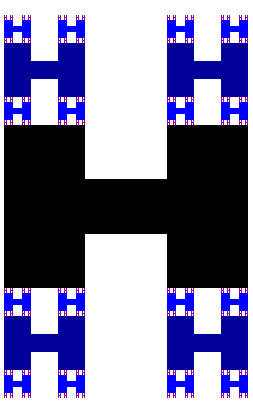
\includegraphics[max width=\textwidth]{hrcrsn}
\end{center}

Kids play with recursions. Draw a big H. Draw 4 smaller H's on the ends of the first one. Draw another 16. Then 64. Everywhere you look the picture is made of the H shape. The picture is recursive.

Some readers may recognise this as a slight elaboration of Cantor's middle-third set, in which the middle third of a line is removed, then the middle third of each of the two remaining lines is removed, and so on as shown below.

\begin{center}
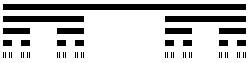
\includegraphics[max width=\textwidth]{cantorm3}
\end{center}

This particular example of a self-similar recursion occurs in numerous writings.

Other well-known examples include the Koch snowflake and the Mandelbrot set.

\section*{NESTED SETS OF RECURSIVE SYSTEMS}
The Viable Systems model is a recursive system.

Originally this was a mathematical model, but happily Beer re-thought his ideas in graphical terms. For many people this is the ideal medium, you can see the problems you are dealing with as a series of drawings, and the complex relationships can be identified within the patterns of lines and loops and arrows.

\textbf{The basis for this recursiveness is the assertion that all viable systems look the same.}

Regardless of its size, all viable organisations look like this; they have an operational part which performs the basic activities, a Metasystem which is charged with providing the services needed by the operational units so that they coheres into a greater whole, and an environment which is in constant interaction with both the operation and the Metasystem. And within these three elements the same rules for Viability can be identified.

\begin{center}
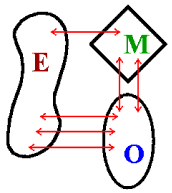
\includegraphics[max width=\textwidth]{vsmbasct}
\end{center}

\textbf{"To cybernetic eyes all viable organisations look exactly the same.
They are all underwritten by the same laws."}

\begin{center}
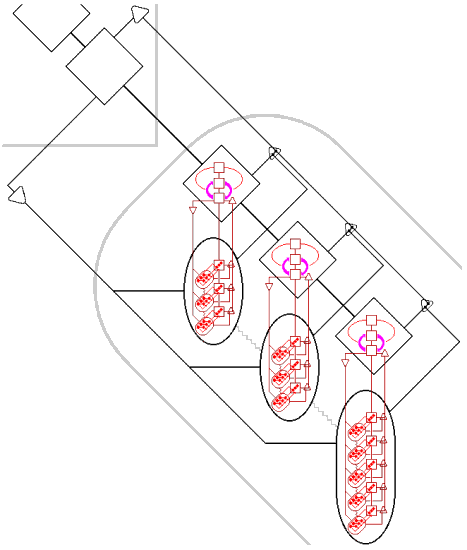
\includegraphics[max width=\textwidth]{vsm5rcsn}
\end{center}

So, if you decide to examine the working of any viable system and zoom in on the operation, you will find a series of smaller viable systems all looking exactly the same as the larger whole.

And just like the automobile investigator, if you decide to raise your perspective, you will find that the system-in-focus is itself embedded in a larger viable system.

Over the last forty years the VSM has been applied to dozens of biological systems and the fundamental recursiveness of nature becomes abundantly clear. From cells to organs to plants and animals, from beehives to oak trees to rainforests, the entire biosphere including the planet itself can best be understood as a set of nested recursive systems.

The same should be true of our businesses and communities and institutions and governments. The current work is concerned with small scale, self-managed viability. Those of you interested in the viability of governments and federations of Nation states and the United Nations are wholeheartedly encouraged to read Beer's work in dozens of publications since 1970.

\section*{FROM THEORY INTO PRACTICE}
This book is designed as a practical guide for people who actually want to use the VSM, and while all this stuff on recursions and cells being the same as the whole planet is all very entertaining, what possible use can it be to anyone concerned with solving organisational problems. Where do you begin?

\subsection*{The First point is focus}
In dealing with a problem it is crucial to identify exactly the boundaries within which the problem is found. There is no point in trying to deal with inefficiency within a particular department unless you have a clear model of the multitude of interactions which will be involved.

Once you have sketched out your organisation as a series of nested viable systems (and it may take some time to clearly disentangle all the recursions) you then have a starting point for your diagnosis.

Other (non-recursive) models don't provide this focus. Either they are concerned with who is responsible to who ... ( so where are the trucks and computers?) or they involve huge flow diagrams covering aspects of several recursive layers, and thus tend to bewilder rather than clarify.

\subsection*{The second point is the universal definition of Viability}
All the Viable systems and all their embedments at all levels throughout the known galaxy have the same structure.

They can all be diagnosed using an absolutely precise definition of Viability.

The practical advantages of this are clear: by disentangling and drawing the recursions you then have the basis for understanding every aspect of the system-in-focus, regardless of its status or size or the power it wields. To cybernetic eyes they are all exactly the same.

\textbf{Beer calls this "the parsimony of natural invariance"}

\subsection*{So where do you begin?}
First of all take pencil and paper and sketch levels of recursion. Much of what follows will involve sketches, so you should get used to dashing off quick drawings. An example is given on the next page.

\section*{DRAWING LEVELS OF RECURSION}
Imagine you have been asked to undertake the study of a large multinational company. You begin by attempting to draw an organisational chart of the whole thing. After several hours you have a several square yards of paper covered with lines and notes and scribbles which is progressively becoming more and more incomprehensible. What can you do?

\textbf{Beer sez "draw the recursions"}

\begin{itemize}
  \item \textbf{Recursion 1 - the whole corporation} sub-systems (system 1) the 3 divisions
  \item \textbf{Recursion 2 - the divisions} system 1 ... 3 companies in this one, 5 in the second
  \item \textbf{Recursion 3 - companies} containing plants
  \item \textbf{Recursion 4 - plants} containing departments
  \item \textbf{Recursion 5 - departments} containing people
\end{itemize}

(Please note: a complete diagram would require the addition of all the other circles. Three divisions, 11 companies, 53 plants and so on.)

\section*{WORKING WITH LEVELS OF RECURSION}
Once you have teased apart the levels of recursion, you can begin to diagnose. This could either be a complete study of the corporation, or as is more likely, it could be a study of a particular problem.

In both cases this involves defining carefully your system in focus. Once this is clear, you can begin to apply the procedures which define the VSM. What are the operational units? Are the four elements of the Metasystem identifiable and working properly? Are the environmental interactions OK?

But you always have to begin with complete clarity about the level of recursion. Each level consists of complete viable systems which are whole and must function (viably) as autonomous entities. If you don't have this clarity, you may try and take into account other parts of the over-all organisation which are not part of the system in focus and which therefore should not be part of this aspect of the diagnosis.

During his work in Chile, Beer projected large diagrams of the various levels of recursion within the Chilean social economy which he used to focus the attention of the people discussing a particular problem. Invariably the discussion would wander up and down the levels of recursion and Beer would say "Excuse me, but this is not part of this recursion and should be put on one side until the current discussion is concluded" (Recursion monitors may well be a crucial job for the next millennia).

The power of all of this is staggering:

\begin{itemize}
  \item As all recursions work in the same way, the tools for dealing with problems at global and international level are exactly the same as those for dealing with a bunch of kids in a youth-club. Once you have an understanding of the VSM, there's nothing to stop you redesigning the United Nations.

  \item Defining the system in focus concentrates your attention on exactly what you need to know. The other 99\% of the organisation can confidently be ignored (at this time) thus giving you a precise, limited environment in which to work. Imagine trying to decide on which part of the many yards of organisational chart you need ....

  \item Working with levels of recursion alone can bring insights. You may find that after a dozen attempts at drawing the levels that the only way to make sense of it all, is to re-think the whole thing in a new way.

\end{itemize}

\section*{CASESTUDY}

\section*{WHY DON'T LARGE GROUPS WORK?}
Take any growing democratic organisation working without authority structures. When numbers are small everything works well. At around 15, problems emerge. At about 20, these problems make it inevitable that smaller functional groupings occur. In the UK problems with organising large groups of people democratically have posed so many problems that some groups have actually shunned expansion to keep their structure small and manageable.


\section*{The VSM looks like this:}
\textbf{The crucial mechanism is thorough discussion between all members.} \textbf{Complete VSM diagnosis reveals a thoroughly workable (albeit unstructured) system.}

\section*{CASE STUDY -}

\section*{WHY DON'T LARGE GROUPS WORK?}

\subsection*{VSM diagnosis}
Look out! Another level of recursion has generated spontaneously!

People arrange themselves into small departmental groups for several reasons ...

\begin{itemize}
  \item they provide a focus for dealing with problems

  \item they get round the horrendous problems of trying to communicate with dozens of other people on a continuous basis

  \item they allow expertise to accumulate in coherent groupings

  \item they work well as teams

\end{itemize}

So how do we do a VSM diagnosis of this?

Some of the members are shown working as five teams, each of which (from the previous page) can be assumed to function as a Viable System It's inevitable that some people's jobs won't fit neatly into this strategy. Someone has to pay the bills, and keep the books. Someone has to ensure that the allocation of personnel to the various groups is handled properly to deal with sickness and holidays.

What is now essential is a look at the next level of recursion up, in which the Operational units are departments, and the job of the Metasystem is to ensure that departments work together as a coherent whole.

\section*{CASE STUDY -}

\section*{WHY DON'T LARGE GROUPS WORK?}

\subsection*{VSM diagram of the next level of recursion up}
\textit{System in focus - the organisation as whole.}

This diagram now represents the whole organisation, and within the Operation there will be five smaller identical diagrams representing the departments (\href{https://vsmg.lrc.org.uk/screen.php?page=recursion#largevsm}{have a look at the large diagram in section above})

The previous section had a brief look at the organisation of one small team and declared it viable. The current job is to look at the whole organisation, ignore the goings on inside the operational units which are not the concern of this level of recursion, and to see how it looks.

The questions are as follows:

The details of this process for Suma are covered in the next chapter - the somewhat staggering conclusion was that almost none of the Metasystemic activity was getting done, and that if the VSM was right, a series of new functions needed to be designed quickly to ensure viability.

Relating this back to the original physiology, the unstructured system had essentially no brains! And all of the problems which had emerged could be neatly allocated to one of the missing systems which Beer maintains are essential for viability.

\section*{CASE STUDY -}

\section*{WHY DON'T LARGE GROUPS WORK?}

\subsection*{Summary}
Everything which happens as a small group grows into a large group can be explained by an analysis based upon a transition from a

two recursions system (people and Business)

to

a three recursions system (people, departments and Business)

At the time this study was undertaken, most people working in the UK had blithely assumed that efficient, people-centred businesses could be built by rejecting hierarchy and basing effective organisation on highly motivated self-managed individuals. The structure would only involve regular meetings and some specialisation. Everything else would take care of itself. Everyone knew it worked for small groups, and it was assumed that it could be extended to a large organisation.

The reality was very different. A paper by an American feminist called "The Tyranny of Structurelessness" argued that in large groups, the lack of structure guaranteed that many individuals would be ignored and that people with dominant personalities would flourish. It became clear that one of the sacred cows of co-operative working had to be slaughtered, and that the kind of egalitarian working practices which were central to our vision could only be ensured through a carefully designed structure.

So the answer to the question is:

\begin{itemize}
  \item It's impossible to involve more than about 7 people in an effective and unstructured organisation because of the practicalities of communication.

  \item Organisations break into small teams, because they work.

  \item This means an extra level of recursion introduces itself.

  \item The business becomes an entirely different animal. Each work team has to work as a viable system in its own right, and a series of new functions become essential as the departments themselves need the services of a Metasystem.

\end{itemize}

Before undertaking this study no-one had suspected that grouping into departments would have any consequences. We work in teams. ... so what?

Thankfully the VSM lays down the rules for dealing with this, and this is developed in the next chapter.

	\chapter{THE LAWS OF VARIETY}\label{THE LAWS OF VARIETY}
%\addcontentsline{toc}{chapter}{Appendix 2. THE LAWS OF VARIETY}
\section*{Overview}
\begin{center}
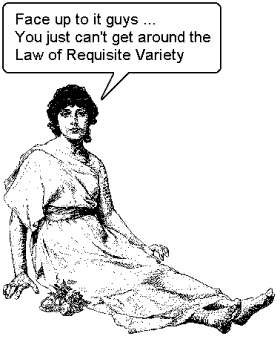
\includegraphics[max width=\textwidth]{sitting3}
\end{center}

The various parts of any system have to be in balance.

Some design procedure is essential in order to ensure that an engine is in balance with the vehicle it drives, or that the heart is designed with sufficient capacity to pump the blood around the organism.

In organisational terms, this (for example) concerns ensuring that the capabilities of the systems which regulate are sufficient to deal with the complexity of the problems which they have to deal with.

Variety is the cybernetician's tool with dealing with these issues.

It's the only method I've so far encountered which encourages you to consider a wide range of solutions and to avoid the knee-jerk reaction of "Well it's obvious ... we need more managers."

\section*{THE LAWS OF VARIETY - WHY BOTHER?}
There is nothing which puts people off VSM ideas quicker than the Laws of Variety. I've met dozens of people who picked up Stafford's books and after a couple of hours put them down in bewilderment and never got any further.

So for those of you who have found yourselves in this position, please consider

\begin{itemize}
  \item Yes, these ideas are new and strange and a little hard to grasp.

  \item There are ways of thinking about all of this which make it easier.

  \item It's worth the effort.

\end{itemize}

All of the crucial aspects of VSM diagnosis and design come from working with variety. The overall vision of self managed, autonomous work-groups and the job of the Metasystem as \textbf{cohesion} comes straight from the variety engineering.

The issue is one of balance. The bits of the VSM have now been discussed and (if you are doing the exercises) identified for your particular enterprise. But what now? You have your Operational elements, and some aspects of systems 2, 3, 4 and 5, but how do you know if the system as a whole is properly designed?

For example, if you've identified System Four as a planning meeting which is held once a year, its highly unlikely that this can carry out the job of ensuring your enterprise can respond to a changing environment. What happens if an opportunity arises? Will you have to wait several months to do something about it? In this case it looks highly likely that your design for a System Four is inadequate, that is, it's \textit{out of balance} with the rest of the structure.

In balancing the parts of you enterprise and (just as importantly) ensuring that your enterprise is in ecological balance with its environment, the following questions must be answered:

\begin{itemize}
  \item Do the operational elements have the ability to respond to changes in their environment?

  \item Do Systems 2 and 3 have the capabilities to carry out their functions of dealing with the inside and now of the enterprise?

  \item Is System 4 designed to be in balance with its internal environment and to deal with the accelerating rate of change in the external environment?

  \item Do the Policy systems work? Are they adequately informed? Are they poised to intervene when necessary?

\end{itemize}

These questions are answered most appropriately by thinking in terms of variety.

\section*{INTRODUCING VARIETY}
The definition of variety is straightforward. It is the number of states in which a system can exist. A switch has a variety of two (on and off) a child has a variety which is enormous.


\section*{VARIETY BALANCES - ASHBY'S LAW}
Consider a steam engine under the control of a Watt governor.

The engine speeds up, the balls fly out, the steam supplied to the engine is cut down. The engine slows down, the balls retract, more steam is let in, the engine speeds up, the balls fly out, and round we go.

It's just the same as a thermostat, or any regulatory device. The Governor is charged with the regulation (control, management) of another system. What can we conclude from all of this?

The complexity of steam engine is defined as the number of possible states in which it can exist. This will mainly be concerned with the different speeds at which it can run, and it will be huge.

In designing the regulator it obvious that it must be able to respond to every state of the engine. (State 23,721, let in 34\% more steam. ... State 349,856 cut down the steam by 56\% ... ) and so on.

In every case, its essential that the regulator can respond to every state in which the steam engine can exist. It would not work if it reached a particular speed which the regulator could not respond to. The system would fail.

So the variety of the Watt Governor must be at least as large as the variety of the steam engine. And in more general terms:

\textbf{\textit{"The variety of a regulator must be at least as large as that of the system it regulates"}}

This statement is usually referred to as \textbf{\href{https://vsmg.lrc.org.uk/screen.php?page=bibliography}{Ashby's Law of Requisite Variety}}, as it says that the regulator must have enough (requisite) variety to adequately do its job.

Assuming that this is clear in the case of the Watt Governor, consider a game of table tennis. Both players have similar variety (they are of similar standards) and each controls the other. The varieties are matched. If one takes lessons, and learns several new techniques, he will increase his variety and the other player will not have enough (requisite) variety to control him.

The other player - who happens to be a cybernetician - thinks "I really have to amplify my variety ... you just can't get around Ashby's's law of Requisite variety!"

And note that while its unlikely that any one table tennis champion would have the variety to beat three simultaneous opponents, chess grand-masters can amplify their variety to such an extent they can match the variety of dozens of opponents.

\section*{OBVIOUS WAYS OF BALANCING VARIETY}
So far we have seen that

\begin{itemize}
  \item variety is a measure of complexity

  \item for a system to work, varieties must be in balance.

\end{itemize}

Some of this was hinted at in the \href{https://vsmg.lrc.org.uk/screen.php?page=2_2cs2}{Suma} case study.

The diagram represents a system where the Metasystem has enough variety to provide cohesion. Or, for every state the operation can exhibit, the Metasystem has the ability to respond. The Metasystem has enough or "requisite variety".

The other diagram showed a huge Operation (more stock lines, more customers, more people, and most importantly cataclysmic increases in permutations) due to exploding variety, and a simultaneous decrease in the size of the Metasystem. Requisite variety had been lost. So the Metasystemic didn't have the capacity to respond to every state of the Operation - it don't work properly. Conflicts were not resolved. No synergy. No forward planning. Policy no longer rounded off the system, so that people could ignore policy constraints.

So what can be done?

Varieties had to be rebalanced, and this can be done in two ways: the variety of the Metasystem can be increased, or the variety of the Operation can be limited.

The usual methods of exercising control are well known. Managers are given more powers and training, (more variety), or the options of Operational workers are restricted (less variety).


\section*{LESS OBVIOUS WAYS OF BALANCING VARIETY}
The power of Variety engineering begins to emerge at this point.p>

If the key is to balance the relative varieties of the Operation and the Metasystem, then new options can be considered.

\subsection*{\textit{Limiting Operational Variety by empowering the workforce}}
If the problem is the exploding variety of the Operation then one solution is to get the people working within the Operation to limit their own variety. Rather than impose an authoritarian regime, you could shrink the size of the Operational problem by getting the people actually doing the work to deal with the problems themselves. Thus self-management, worker empowerment and all the Tom Peters stuff about training production line staff to do statistical analysis of production figures.

"GRASP THIS NETTLE

The management of the system-in-focus is in principle unable to entertain the variety generated by any one (never mind all) of its subsidiary viable systems that constitute System One.

The beginnings of a theory of autonomy, of decentralisation lie in this simple fact"

(Beer "\href{https://vsmg.lrc.org.uk/screen.php?=bibliography}{Diagnosing the System}" p.37)

\subsection*{\textit{Balancing Varieties using Information Processing}}
The conclusion is encouraging: a well designed information system can be used as an alternative to authoritarian control. It can enhance self-managed, autonomous individuals.

\section*{A NEW UNIVERSE OF POSSIBILITIES}

\section*{DESIGN BY VARIETY ENGINEERING}
Variety engineering is the term used to describe the technique of looking at the multitude of ways that varieties can be manipulated in designing effective organisations.

The essence of this approach is to provide a set of tools (involving variety) which gives you a whole range of new options.

The trick is to find a way of skinning the cat, which does minimal harm to the cat.

"Managerial, operational and environmental varieties should be designed to balance, with minimal damage to people and to cost."

(Beer "\href{https://vsmg.lrc.org.uk/screen.php?=bibliography}{The Heart of Enterprise}" p.97)

This is a slightly abridged version of Beer's First Principle of Organisation. If it's accepted that you can choose between a philosophy involving bullies, soldiers, and blind obedience, or of working a new universe of possibilities including autonomy and carefully constructed information systems, then the way forward (for most of us) is clear.

Many of the basic premises of co-operation can be re-interpreted in this light. Basing an organisation on self-managed individuals, rather than the cog-in-machine vision of production line techniques, becomes a sound working practice in terms of variety engineering. The vast majority of problems are dealt with at this level, huge quantities of variety are absorbed by intelligent behaviour at the operational level, and the remaining problems ( sometimes called residual variety) can be mopped up easily by the Metasystem.

In more traditional terms the argument can be expressed as follows:

\textbf{\textit{"If you empower the workers to solve their own problems, then the people whose job it is to manage these workers will have almost nothing to do."}}

The politics of all this are endless. In terms of variety engineering its simply a question of deciding which of the many methods of balancing varieties are the most effective. Interestingly enough the most appropriate solutions generally seem to suggest more libertarian protocols.

\section*{SUMMARY}
Variety is a measure of complexity.

Ashby's Law states that the variety of a system which regulates has to equal the variety of the system it is regulating.

This can be expressed in a number of ways. It's often expressed as:

"Only Variety can absorb variety"

In organisational terms it means that the capabilities of the regulators, have to balance the complexity of the situation they are charged with regulating.

This regulation could be the traditional view of management, or it could be the regulation of a jazz band where the rules by which the music unfolds are under the control of the people making it. Or the regulation of body temperature. In all these cases Ashby's Law is pertinent.

If the systems which regulate don't have enough (or requisite) variety to match the complexity of the regulated, then regulation will fail. The system will be out of control.

Variety Engineering is the manipulation of varieties in whatever way is most appropriate to restore the balance between regulator and regulated.

In practical terms the consideration of organisational problems in terms of variety provides a huge new battery of possibilities which are unavailable to other techniques.

\textit{\textbf{Some level of understanding of these ideas is essential for the rest of this book. However, given the difficulty many people have with variety, I will usually include a re-interpretation using more conventional language.}}

If the entire concept leaves you completely bewildered, try re-reading this chapter or one of Beer's many introductions to variety (or the original treatment in \textbf{\href{https://vsmg.lrc.org.uk/screen.php?page=bibliography}{An Introduction to Cybernetics}} by \textbf{W. Ross Ashby} - Chapman and Hall, 1956). (The language used to write about systems has changed over the years but, despite that, this classic textbook is still as useful as ever. It was written to be accessible to as wide a variety of readers as possible and is still the only book to cover the fundamentals of cybernetics with a clear, step-by-step approach. In recognition of this book's importance, the \href{http://pespmc1.vub.ac.be/}{Principia Cybernetica Web} has made a \href{http://pespmc1.vub.ac.be/ASHBBOOK.html}{PDF version} available on-line.)
...
\end{appendices}

\end{document}